\documentclass[aoas]{imsart}
\usepackage{amssymb, amsthm, amsmath}
\usepackage{bm}
\usepackage{graphicx}
\usepackage[authoryear]{natbib}
\usepackage{bm}
\usepackage{verbatim}
\usepackage{lineno}
\usepackage{times}
\usepackage{soul}
\usepackage{color}
\usepackage{enumerate}
% \usepackage{setspace}
\usepackage{times}
\usepackage{changepage}
\usepackage{multirow}
\usepackage{booktabs}
\usepackage{pdflscape}
\usepackage{hyperref}

% \usepackage[left=1in,top=1in,right=1in]{geometry}
% \pdfpageheight 11in
% \pdfpagewidth 8.5in
% \linespread{2.0}
\setcitestyle{notesep={; }}

\startlocaldefs
\newcommand{\btheta}{ \mbox{\boldmath $\theta$}}
\newcommand{\bmu}{ \mbox{\boldmath $\mu$}}
\newcommand{\balpha}{ \mbox{\boldmath $\alpha$}}
\newcommand{\bbeta}{ \mbox{\boldmath $\beta$}}
\newcommand{\bdelta}{ \mbox{\boldmath $\delta$}}
\newcommand{\blambda}{ \mbox{\boldmath $\lambda$}}
\newcommand{\bgamma}{ \mbox{\boldmath $\gamma$}}
\newcommand{\brho}{ \mbox{\boldmath $\rho$}}
\newcommand{\bpsi}{ \mbox{\boldmath $\psi$}}
\newcommand{\bepsilon}{ \mbox{\boldmath $\epsilon$}}
\newcommand{\bomega}{ \mbox{\boldmath $\omega$}}
\newcommand{\bOmega}{ \mbox{\boldmath $\Omega$}}
\newcommand{\bDelta}{ \mbox{\boldmath $\Delta$}}
\newcommand{\bSigma}{ \mbox{\boldmath $\Sigma$}}
\newcommand{\bPsi}{\mbox{\boldmath $\Psi$}}
\newcommand{\bOne}{\mbox{\boldmath $1$}}
\newcommand{\omu}{\overline{\mu}}
\newcommand{\oSigma}{\overline{\Sigma}}
\newcommand{\Yt}{{\tilde Y}}
\newcommand{\bA}{ \mbox{\bf A}}
\newcommand{\bP}{ \mbox{\bf P}}
\newcommand{\bx}{ \mbox{\bf x}}
\newcommand{\bX}{ \mbox{\bf X}}
\newcommand{\bB}{ \mbox{\bf B}}
\newcommand{\bT}{ \mbox{\bf T}}
\newcommand{\bZ}{ \mbox{\bf Z}}
\newcommand{\by}{ \mbox{\bf y}}
\newcommand{\bY}{ \mbox{\bf Y}}
\newcommand{\bz}{ \mbox{\bf z}}
\newcommand{\bh}{ \mbox{\bf h}}
\renewcommand{\bm}{ \mbox{\bf m}}
\newcommand{\br}{ \mbox{\bf r}}
\newcommand{\bt}{ \mbox{\bf t}}
\newcommand{\bk}{\mbox{\bf k}}
\newcommand{\bs}{ \mbox{\bf s}}
\newcommand{\bb}{ \mbox{\bf b}}
\newcommand{\bL}{ \mbox{\bf L}}
\newcommand{\bu}{ \mbox{\bf u}}
\newcommand{\bv}{ \mbox{\bf v}}
\newcommand{\bV}{ \mbox{\bf V}}
\newcommand{\bW}{ \mbox{\bf W}}
\newcommand{\bG}{ \mbox{\bf G}}
\newcommand{\bH}{ \mbox{\bf H}}
\newcommand{\bw}{ \mbox{\bf w}}
\newcommand{\bo}{ \mbox{\bf o}}
\newcommand{\bfe}{ \mbox{\bf e}}
\newcommand{\iid}{\stackrel{iid}{\sim}}
\newcommand{\ind}{\stackrel{ind}{\sim}}
\newcommand{\dd}{\; \text{d} }
\newcommand{\ddd}{\text{d} }
\newcommand{\indep}{\stackrel{indep}{\sim}}
\newcommand{\converged}{\stackrel{d}{\rightarrow}}
\newcommand{\goesto}[1]{\stackrel[#1]{}{\longrightarrow}}
\newcommand{\calR}{{\cal R}}
\newcommand{\calG}{{\cal G}}
\newcommand{\calD}{{\cal D}}
\newcommand{\calS}{{\cal S}}
\newcommand{\calB}{{\cal B}}
\newcommand{\calA}{{\cal A}}
\newcommand{\calT}{{\cal T}}
\newcommand{\calO}{{\cal O}}
\newcommand{\argmax}{{\mathop{\rm arg\, max}}}
\newcommand{\argmin}{{\mathop{\rm arg\, min}}}
\newcommand{\Frechet}{\mbox{Fr$\acute{\mbox{e}}$chet }}
\newcommand{\Matern}{\mbox{Mat$\acute{\mbox{e}}$rn }}
\newcommand{\ballunion}{B_a(\bs_1) \cup B_b(\bs_2) }

\newcommand{\alphahat}{\hat{\alpha}}

\newcommand{\eref}[1]{(\ref{#1})}
\newcommand{\fref}[1]{Figure~\ref{#1}}
\newcommand{\tref}[1]{Table~\ref{#1}}
\newcommand{\sref}[1]{Section~\ref{#1}}
\newcommand{\aref}[1]{Appendix~\ref{#1}}

\newcommand{\beq}{ \begin{equation}}
\newcommand{\eeq}{ \end{equation}}
\newcommand{\beqn}{ \begin{eqnarray}}
\newcommand{\eeqn}{ \end{eqnarray}}

\newcommand*\patchAmsMathEnvironmentForLineno[1]{%
  \expandafter\let\csname old#1\expandafter\endcsname\csname #1\endcsname
  \expandafter\let\csname oldend#1\expandafter\endcsname\csname end#1\endcsname
  \renewenvironment{#1}%
     {\linenomath\csname old#1\endcsname}%
     {\csname oldend#1\endcsname\endlinenomath}}% 
\newcommand*\patchBothAmsMathEnvironmentsForLineno[1]{%
  \patchAmsMathEnvironmentForLineno{#1}%
  \patchAmsMathEnvironmentForLineno{#1*}}%
\AtBeginDocument{%
\patchBothAmsMathEnvironmentsForLineno{equation}%
\patchBothAmsMathEnvironmentsForLineno{align}%
\patchBothAmsMathEnvironmentsForLineno{flalign}%
\patchBothAmsMathEnvironmentsForLineno{alignat}%
\patchBothAmsMathEnvironmentsForLineno{gather}%
\patchBothAmsMathEnvironmentsForLineno{multline}%
}

\endlocaldefs


\begin{document} % \linenumbers
\begin{frontmatter}
\title{Exploration and inference in spatial extremes using empirical basis functions}

\author{\fnms{Samuel A.} \snm{Morris}\thanksref{ncsu}\ead[label=e1]{samorris@ncsu.edu}},
\author{\fnms{Brian J.} \snm{Reich}\thanksref{ncsu}\ead[label=e2]{bjreich@ncsu.edu}}
\address{\printead{e1}}
\and
\author{\fnms{Emeric} \snm{Thibaud}\thanksref{csu}\ead[label=e3]{emericemail}}

\runauthor{S. Morris et al.}
\affiliation{North Carolina State University\thanksmark{ncsu} and Colorado State University\thanksmark{csu}}

\begin{abstract}
  Abstract goes here

\end{abstract}

\begin{keyword}
  \kwd{non-stationary data analysis}
  \kwd{max-stable process}
  \kwd{spectral representation}
  \kwd{dimension reduction}
\end{keyword}


\end{frontmatter}

\section{Introduction}\label{ebs:intro}

The spatial Extreme Value Analysis (EVA) literature is expanding rapidly \citep{Davison2012} to meet the demands of researchers to improve estimates of rare-event probabilities by borrowing information across space and to estimate the probability of extreme events occurring simultaneously at multiple locations.
Environmental datasets commonly include observations from hundreds or thousands of locations, and advanced tools are required to explore and analyze these data.
For Gaussian data, Principle Components Analysis \citep[PCA]{Everitt2008}, also known as Empirically Orthogonal Functions \citep[EOF]{Toggweiler2001}, has proven to be a powerful tool to study correlation between spatial locations; understand the most important large-scale spatial features; and reduce the dimension of the problem to allow for simple computation even for massive datasets.
Computation and exploration are arguably more difficult for EVA than Gaussian data, yet to our knowledge no tool analogous to spatial PCA has been developed for EVA.

In EVA, extremes are separated from the bulk of the distribution by either analyzing only points above a threshold or block maximums \citep{Coles2001}, e.g., the annual maximum of the daily precipitation.
A natural spatial model for block maximum at several spatial locations is the max-stable process, which, under certain conditions, arises as the limit of the location-wise maximum of infinitely-many spatial processes \citep{deHaan2006}.
Max-stable processes were also used to model spatial exceedances over a high threshold \citep{Thibaud2013,Huser2014}.
\Citet{deHaan1984} showed that any max-stable process can be represented in terms of a countable number of spatial processes (e.g., stationary log Gaussian processes), and a finite truncation of this representation has been used for conditional simulation \citep{Wang2011}.
Fully-Bayesian analysis using max-stable processes is cumbersome for large data sets \citep{Wadsworth2014,Thibaud2013a}.
One option is to use non-max-stable models that retain extremal dependence such as the \skewt{} process in \citep{Morris2016}.
Alternatively, \citet{Reich2012} propose a low-rank method based on spatial kernel functions, and others have used pairwise \citep{Padoan2010,Huser2014} and trivariate \citep{Genton2011} likelihood methods for parameter estimation.

In this paper we propose an empirical basis function (EBF) approach that builds on a finite truncation of the spectral representation, and develops a method-of-moments estimator for the underlying spatial processes.
Unlike PCA/EOFs, but similar to dictionary learning \citep{Mairal2014} and non-negative matrix factorizations \citep{Lee1999}, the EBFs are not orthogonal.
Nonetheless these spatial functions can be plotted for exploratory analysis to reveal important spatial trends.
In addition to exploratory analysis, we show that the EBFs can be used for Bayesian inference on the marginal parameters at each location, modeling spatial dependence, and to test for covariate effects.
By basing the spatial dependence on EBFs, the resulting spatial analysis does not require dubious assumptions such as stationarity.
In addition, a Bayesian analysis for either block-maximum or point above a threshold is computationally feasible for large datsets because the entire spatial process is represented by a small number of basis functions.

The paper proceeds as follows.
In \sref{ebs:model} we present the low-rank model. \sref{ebs:estimation} describes the algorithm used to estimate the spatial basis functions, and \sref{ebs:MCMC} describes the model fit using Markov chain Monte Carlo (MCMC) methods.
In \sref{ebs:analysis} we demonstrate the use of the EBFs for an analysis of precipitation data in the eastern U.S. Lastly in \sref{ebs:con} we give some summary conclusions and a brief discussion of the findings.

\section{Model}\label{ebs:model}

Let $Y_{t}(\bs)$ be the observation at spatial location $\bs$ and time $t$.  We temporarily drop the subscript $t$ and describe the model for the process $Y(\bs)$ for a single time point, but return to the spatiotemporal notation in \sref{ebs:estimation}.
To focus attention on the extreme values, we emphasize the statistical model for exceedances above a location-specific threshold $T(\bs)$.
We begin by specifying a spatial model for the complete data $Y(\bs)$ and then use the censored likelihood defined by $T(\bs)$ for inference as described in \sref{ebs:MCMC}.
Although the model presented implements a censored likelihood, the model also can fit uncensored data (such as block-maxima) by setting $T(\bs) = -\infty$.

Spatial dependence is captured by modeling $Y(\bs)$ as a max-stable process \citep{deHaan2006}.
Max-stable processes have generalized extreme value (GEV; see \aref{eba:GEV}) marginal distribution.
The GEV has three parameters: location $\mu(\bs)$; scale $\sigma(\bs)$; and shape $\xi(\bs)$.
Spatial dependence is present both in the GEV parameters but also the standardized residual process
\begin{align} \label{ebeq:Y2Z}
 Z(\bs) = \left\{1+\frac{\xi(\bs)}{\sigma(\bs)}\left[Y(\bs) - \mu(\bs)\right]\right\}^{1/\xi(\bs)},
\end{align}
which has unit $\Frechet$ (i.e., GEV with location, scale, and shape all equal one) marginal distribution for all $\bs$.

Our objective is to identify a low-rank model for the spatial dependence of $Z(\bs)$.
\Citet[Chapter 9]{deHaan1984} show that any max-stable process can be written as
\begin{align} \label{ebeq:spectral}
  Z(\bs) = \bigvee_{l = 1}^{\infty} B(\bs, \bk_l)A_{l}
\end{align}
where the functions $B(\bs, \bk_l)$ satisfy $B(\bs, \bk_l) > 0$ for all $\bs$ and $\int B(\bs, \bk_l) \dd \bk_l = 1$ for all $\bs$, and $(\bk_l, A_l)$ for $l=1,\ldots,\infty$ are a Poisson process with intensity measure $\dd A \dd \bk/A^2$.
In many representations of max-stable process, such as \citet{Smith1990} and \citet{Reich2012}, the $\bk_l$ are spatial locations that represent the center of process $l$; however, in our proposed method the basis functions are not associated with one particular location and so to simplify notation we let $B_l(\bs) = B(\bs; \bk_l)$

To arrive at a low-rank model, we assume there are a finite and known number of spatial basis functions $B_1(\bs), \ldots, B_L(\bs)$ that explain the important spatial variation in the process.
As in de Haan's expansion, the basis functions are restricted so that $B_l(\bs) > 0$ and $\displaystyle \sum_{l = 1}^L B_l(\bs) = 1$ for all $\bs$.
Because it is unrealistic to assume that realizations of $Z$ are exactly functions of $L$ basis functions, we include independent error variables $\epsilon(\bs)$ to capture variation not explained by the $B_l(\bs)$.
We follow \citet{Reich2012} and decompose $Z(\bs)$ as $Z(\bs)=\theta(\bs)\varepsilon(\bs)$ where $\theta(\bs)$ is a spatial process and $\varepsilon(\bs)\iid$ GEV$(1,\alpha,\alpha)$ is independent error.
The spatial component is
\begin{align} \label{ebeq:theta}
  \theta(\bs) = \left(\sum_{l=1}^LB_{l}(\bs)^{1/\alpha}A_{l}\right)^{\alpha}.
\end{align}
If $B_{l}(\bs)>0$, $\displaystyle \sum_{l=1}^LB_{l}(\bs)=1$ for all $\bs$, and the $A_{l}$ have positive stable (PS; \aref{eba:gridapprox}) distribution \mbox{$A_{l}\iid$ PS$(\alpha)$}, then $Z(\bs)$ is max-stable and has unit $\Frechet$ marginal distributions.

Extremal spatial dependence for max-stable processes can be summarized by the extremal coefficient \citep[EC]{Schlather2003} $\vartheta(\bs_1, \bs_2)\in[1,2]$, where
\begin{align} \label{ebeq:ECdev}
  \mbox{Prob}[Z(\bs_1)<c, Z(\bs_2)<c] = \mbox{Prob}[Z(\bs_1)<c]^{\vartheta(\bs_1,\bs_2)}.
\end{align}
For the PS random effects model the EC has the form
\begin{align} \label{ebeq:EC}
   \vartheta(\bs_1,\bs_2) = \sum_{l=1}^L \left[B_{l}(\bs_1)^{1/\alpha}+B_{l}(\bs_2)^{1/\alpha}\right]^\alpha.
\end{align}
In particular, $\vartheta(\bs,\bs) = 2^{\alpha}$ for all $\bs$.

\section{Estimating the basis functions} \label{ebs:estimation}

To estimate the extremal coefficient function, we consider the process at $n_s$ spatial locations $\bs_1,\ldots,\bs_{n_s}$ and $n_t$ times $t=1,\ldots,n_t$.
The basis functions are fixed over time, but the random effects and errors are independent over time.
That is
\begin{align}
  Z_t(\bs) = \theta_t(\bs) \epsilon_t(\bs) \quad \mathrm{where} \quad \theta_t(\bs) = \left(\displaystyle \sum_{l=1}^L B_{l}(\bs)^{1/\alpha}A_{lt}\right)^{\alpha},
\end{align}
$A_{lt} \iid$ PS$(\alpha)$, and $\epsilon_t(\bs) \iid$ GEV$(1, \alpha, \alpha)$.
Denote $Y_t(\bs_i) = Y_{it}$, $B_l(\bs_i) = B_{il}$, $T(\bs_i)=T_i$, and $\vartheta(\bs_i,\bs_j) = \vartheta_{ij}$.

In this section we develop an algorithm to estimate the spatial dependence parameter $\alpha$ and the $n_s\times L$ matrix $\bB = \{B_{il}\}$.
% Given these parameters, we insert them into our model and proceed with Bayesian analysis as described in \sref{ebs:MCMC}.
Our algorithm has the following steps:
\begin{enumerate}[(1)]
  \item Obtain an initial estimate of the extremal coefficient for each pair of locations, ${\hat \vartheta}_{ij}$.
  \item Spatially smooth these initial estimates ${\hat \vartheta}_{ij}$ using kernel smoothing to obtain ${\tilde \vartheta}_{ij}$.
  \item Estimate the spatial dependence parameters by minimizing the difference between model-based coefficients, $\vartheta_{ij}$, and smoothed coefficients, ${\tilde \vartheta}_{ij}$.
\end{enumerate}

% Use for thesis
% The first-stage estimates are obtained using an empirical estimate as follows.
% To estimate the spatial dependence we first remove variation in the marginal distribution.
% Let $U_{it} = \sum_{k=1}^{n_t} I[Y_{ik}<Y_{it}]/n_t$, so that the $U_{it}$ are approximately uniform at each location.
% Then for some extreme probability $q\in(0,1)$, solving \eref{ebeq:ECdev} suggests the estimate
% \begin{align}\label{ebeq:EChat0}
%    {\hat \vartheta}_{ij}(q) = \frac{\log[Q_{ij}(q)]}{\log(q)},
% \end{align}
% where $Q_{ij}(q) = \sum_{t=1}^{n_t}I[U_{it}<q,U_{jt}<q]/n_t$ is the sample proportion of the time points at which both sites are less than $q$.
% Since all large $q$ give valid estimates, we average over a grid of $q$ with $q_1< \cdots <q_{n_q}$
% \begin{align} \label{ebeq:EChat1}
% {\hat \vartheta}_{ij} = \frac{1}{n_q}\sum_{j=1}^{n_q}{\hat \vartheta}_{ij}(q_j).
% \end{align}

% Use for paper
The first-stage estimates are obtained from the estimator of \citet{Schlather2003} using the \texttt{fmadogram} function in the \texttt{SpatialExtremes} \citep{Ribatet2015} package of \texttt{R} \citep{Rmanual}.
Assuming the true EC is smooth over space, the initial estimates ${\hat \vartheta}_{ij}$ can be improved by smoothing.
Let
\begin{align} \label{ebeq:EChat2}
  {\tilde \vartheta}_{ij} = \frac{\sum_{u=1}^{n_s}\sum_{v=1}^{n_s} w_{iu}w_{jv}{\hat \vartheta}_{uv}}
  {\sum_{u=1}^{n_s}\sum_{v=1}^{n_s} w_{iu}w_{jv}},
\end{align}
where $w_{iu} = \exp[-(||\bs_i-\bs_u'||/\phi)^2])$ is the Gaussian kernel function with bandwidth $\phi$.
The elements ${\hat \vartheta}_{ii}$ do not contribute any information as ${\hat \vartheta}_{ii}=1$ for all $i$ by construction.
To eliminate the influence of these estimates we set $w_{ii}=0$.
However, this approach does give imputed values ${\tilde \vartheta}_{ii}$, which provide information about small-scale spatial variability.

The dependence parameters $B_{lt}$ and $\alpha$ are estimated by comparing estimates ${\tilde \vartheta}_{ij}$ with the model-based values $\vartheta_{ij}$.
For all $i$, $\vartheta_{ii} = 2^{\alpha}$, and therefore we set $\alpha$ to $\alphahat = \log_2\left(\displaystyle \sum_{i=1}^{n_s}{\tilde \vartheta}_{ii}/n_s\right)$.
Given $\alpha=\alphahat$, it remains to estimate $\bB$.
Similarly to \citet{Smith1990} for a stationary max-stable process, we use squared-error loss, so the estimate $\hat{\bB}$ is the minimizer of
\begin{align} \label{ebeq:Bhat}
\sum_{i<j} \left({\tilde \vartheta}_{ij} - \vartheta_{ij}\right)^2
  =
  \sum_{i<j} \left({\tilde \vartheta}_{ji} - \sum_{l=1}^L \left[B_{il}^{1/\alphahat} + B_{jl}^{1/\alphahat} \right]^{\alphahat}\right)^2
\end{align}
under the restrictions that $B_{il}\ge 0$ for all $i$ and $l$ and $\displaystyle \sum_{l=1}^LB_{il}=1$ for all $i$.
Since the minimizer of \eref{ebeq:Bhat} does not have a closed form, we use block coordinate descent to obtain ${\hat \bB}$.
We cycle through spatial locations and update the vectors $\left(\hat{B}_{i1},\ldots,\hat{B}_{iL}\right)$ conditioned on the values for the other location and repeat until convergence.
At each step, we use the restricted optimization routine in the \texttt{R} function \texttt{optim}.
This algorithm gives estimates of the $B_{il}$ at the $n_s$ data locations, but is easily extended to all $\bs$ for spatial prediction.
The kernel smoothing step ensures that the estimates for $\hat{B}_{il}$ are spatially smooth, and thus interpolation of the $\hat{B}_{il}$ gives spatial functions $\hat{B}_l(\bs)$.

These functions provide useful exploratory data analysis techniques.
Maps of $\hat{B}_l(\bs)$ show important spatial features in the extremal dependence.
Furthermore, they allow for a non-stationary spatial dependence structure.
The relative contribution of each term can be measured by
\begin{align} \label{ebeq:v}
v_l = \frac{1}{n_s}\sum_{i=1}^{n_s}{\hat B}_{il}.
\end{align}
Since $\displaystyle \sum_{l=1}^L{\hat B}_{il}=1$ for all $i$, we have $\displaystyle \sum_{l=1}^Lv_l = 1$.
Therefore, terms with large $v_l$ are the most important.
The order of the terms is arbitrary, and so we reorder the terms so that $v_1\ge \cdots \ge v_L$.

\section{Bayesian implementation details}\label{ebs:MCMC}

For our data analysis in \sref{ebs:analysis} we allow the GEV location and scale parameters, denoted $\mu_t(\bs)$ and scale $\sigma_t(\bs)$ respectively, to vary with space and time.
The model we choose is as follows
\begin{align}\label{ebeq:GPprior}
  \mu_t(\bs) &= \beta_{1, \text{int}}(\bs) + \beta_{1, \text{time}}(\bs) t\\
  \log[\sigma_t(\bs)] &= \beta_{2, \text{int}}(\bs) + \beta_{2, \text{time}}(\bs) t
\end{align}
where
\begin{align} \label{ebeq:GPhyper}
  \beta_{1, \text{int}}(\bs) &\sim \text{N}(\mu^{\phantom{2}}_{1, \text{int}} \bOne, \sigma^2_{1, \text{int}} \bSigma) \quad &\beta_{1, \text{time}}(\bs) &\sim \text{N}(\mu^{\phantom{2}}_{1, \text{time}} \bOne, \sigma^2_{1, \text{time}} \bSigma) \\
  \beta_{2, \text{int}}(\bs) &\sim \text{N}(\mu^{\phantom{2}}_{2, \text{int}} \bOne, \sigma^2_{2, \text{int}} \bSigma) \quad &\beta_{2, \text{time}}(\bs) &\sim \text{N}(\mu^{\phantom{2}}_{2, \text{time}} \bOne, \sigma^2_{2, \text{time}} \bSigma) \nonumber
\end{align}
are Gaussian process priors and $\bSigma$ is an exponential spatial correlation matrix obtained from \mbox{$\rho(h) = \exp\left\{- \frac{h}{\phi}\right\}$} where $h = ||\bs_1 - \bs_2||$ is the Euclidean distance between sites $\bs_1$ and $\bs_2$.
The GEV shape parameter $\xi$ is held constant over space and time because this parameter is challenging to estimate.
Collectively, let the marginal GEV parameters at location $i$ and time $t$ be $\Theta_{it} = \{\mu_{it},\sigma_{it},\xi\}$ where $\mu_{it} = \mu_t(\bs_i)$ and $\sigma_{it} = \sigma_t(\bs_i)$.

As shown in \citet{Reich2012}, the uncensored responses $Y_{t}(\bs)$ are conditionally independent given the spatial random effects, with conditional distribution
\begin{align} \label{ebeq:Ycond}
   Y_{it}|\theta_{it},\Theta_{it} \ind \mathrm{GEV}(\mu^*_{it}, \sigma_{it}^*,\xi^*),
\end{align}
where $\mu_{it}^* = \mu_{it} + \frac{\sigma_{it}}{\xi}(\theta_{it}^\xi - 1)$,
$\sigma_{it}^* = \alpha\sigma_{it}\theta_{it}^\xi$, and $\xi^* = \alpha\xi$.
Therefore, the conditional likelihood conveniently factors across observations; marginalizing over the random effect $\theta_{it}$ induces extremal spatial dependence.
To focus on the extreme values above the local threshold $T_i$, we use the censored likelihood
\begin{align} \label{ebeq:g}
d(y;\theta_{it},\Theta_{it}, T_i)  = \begin{cases}
  F(y;\mu_{it}^*,\sigma_{it}^*,\xi^*) & y \le T_i \\
  f(y;\mu_{it}^*,\sigma_{it}^*,\xi^*) & y>T_i,
\end{cases}
\end{align}
where $F$ and $f$ are the GEV distribution and density functions, respectively, defined in \aref{eba:GEV}.

In summary, given the estimates of $\alpha$ and $\bB$, the hierarchical model is
\begin{align} \label{ebeq:bayesmodel}
  Y_{it} |\theta_{ij} &\indep d(y;\theta_{it},\Theta_{it}, T_i) \\
  \theta_{it} &= \left(\sum_{l=1}^L{\hat B}_{il}^{1/\alphahat}A_{lt}\right)^{\alphahat}
  \text{\ \ \ where \ \ \ }
  A_{lt} \iid PS(\alphahat)\nonumber\\
  \mu_{it} &= \beta_{1, \text{int}}(\bs_i) + \beta_{1, \text{time}}(\bs_i) t \nonumber \\
  \log(\sigma_{it}) &= \beta_{2, \text{int}}(\bs) + \beta_{2, \text{time}}(\bs) t. \nonumber
\end{align}
We estimate parameters $\Theta = \left\{A_{lt}, \bbeta_1, \bbeta_2, \xi \right\}$ using Markov chain Monte Carlo methods.
We use a Metropolis-Hastings algorithm to update the model parameters with random walk candidate distributions for all parameters.
The PS density is challenging to evaluate as it does not have a closed form.
One technique to avoid this complication is to incorporate auxiliary random variables \citep{Stephenson2009}, but we opt for a numerical approximation to the integral as described in \aref{eba:gridapprox}.
The hyperparameters $\mu_{1, \text{int}}$, $\mu_{1, \text{time}}$, $\mu_{2, \text{int}}$, $\mu_{2, \text{time}}$ and $\sigma^2_{1, \text{int}}$, $\sigma^2_{1, \text{time}}$, $\sigma^2_{2, \text{int}}$, $\sigma^2_{2, \text{time}}$ are updated using Gibbs sampling since their prior distributions are conjugate.

The first-stage estimate of the extremal coefficients has two tuning parameters: the kernel bandwidth $\phi$, and the number of terms $L$.
In \sref{ebs:analysis} we explore a few possibilities for $L$ and discuss sensitivity to this choice.
The second-stage Bayesian analysis requires selecting thresholds $T_i,\ldots,T_{n_s}$.  For this we use spatially smoothed sample quantiles.
That is, we set $T_i$ to the 0.95 quantile of the $Y_{it}$ and its five nearest neighbors.

\section{Data analysis}\label{ebs:analysis}

In this section, we illustrate our method with an analysis of block maxima precipitation data in the eastern U.S.
We compare our method with results from a more na\"{i}ve approach that uses standardized Gaussian kernels for the spatial basis functions.

\subsection{Gaussian kernel basis functions}
\label{ebs:gskfunc}

To provide a comparison of our model with another approach, we also fit a model that uses standardized Gaussian kernels for the spatial basis functions \citep{Reich2012}.
In this method, \citeauthor{Reich2012} introduce a set of $\bk_1, \ldots, \bk_L$ spatial knots and use standardized Gaussian kernel functions (GSK; see \aref{eba:gskfunctions}) instead of using EBFs for the $\hat{B_l}(\bs)$.
For the comparison between EBF and GSK methods, we use the same number of basis functions.
We obtain estimates of the kernel bandwidth $\hat{\rho}$ and spatial dependence $\hat{\alpha}$, using the same least squares minimization as with the EBF method, and treat these as fixed in the MCMC.

%\subsection{Analysis of extreme Georgia fires}\label{ebs:georgia}
%
%The dataset used for our application is composed of yearly acreage burned due to wildfires for each county in Georgia from 1965 -- 2014 (\url{http://weather.gfc.state.ga.us/FireData/}).
%\fref{ebfig:firets25} shows the time series of $\log$(acres burned) for 25 randomly selected counties.
%Based on this plot and other exploratory analysis, we see no evidence of non-linear trends and proceed with linear time trends for the GEV location and scale parameters.
%
%\begin{figure}[htbp]  % markdown/eda/eda-plotting.R
%  \centering
%  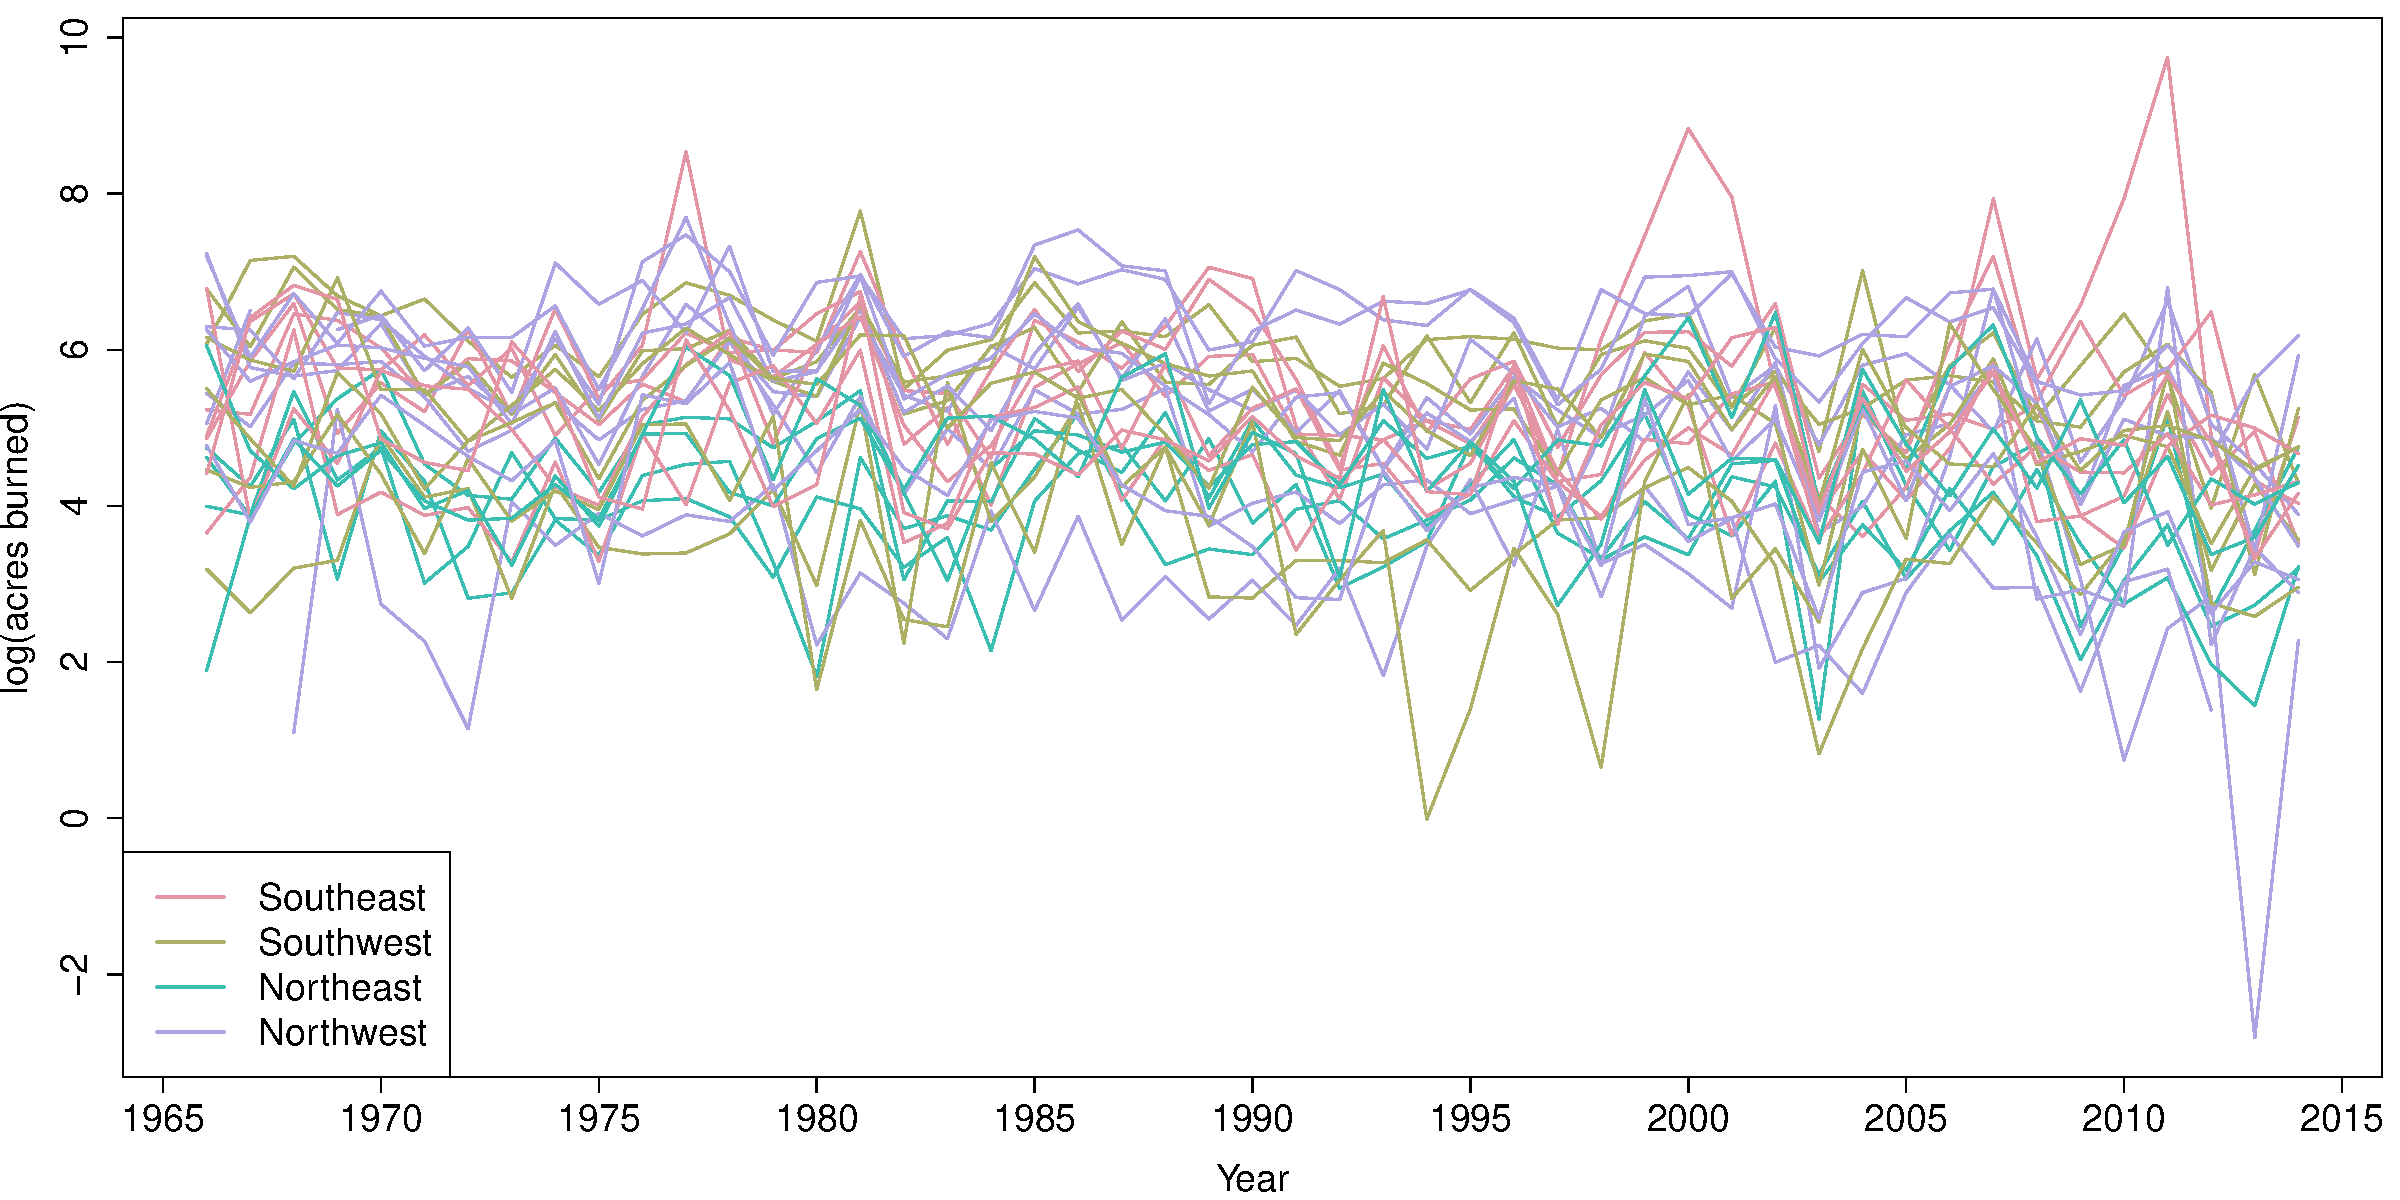
\includegraphics[width=0.55\linewidth]{plots/fire-spag-rand-25}
%  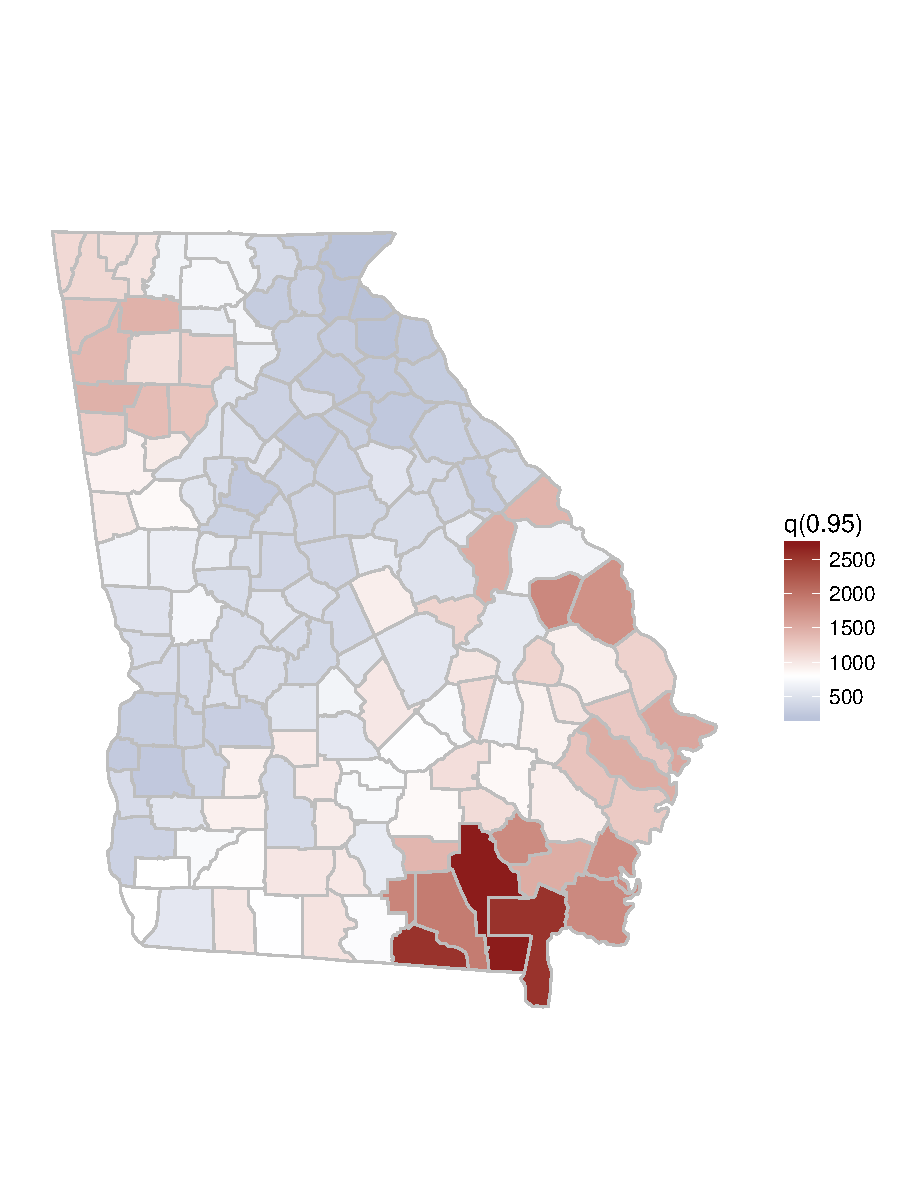
\includegraphics[width=0.44\linewidth, trim = 0 8em 0 10em]{plots/fire-spatial-q95.pdf}
%  \caption{Time series of log acres burned for 25 randomly selected counties with colors coding the county's quadrant (left), and spatially smoothed threshold values, $T_i$ for each county (right).}
%  \label{ebfig:firets25}
%\end{figure}
%
%We estimate the extremal coefficient function $\hat{\theta}_{ij}$ by setting $q_1 = 0.90$ and using $n_q = 100$.
%With more data, it would possible to increase $q_1$, but we set $q_1 = 0.90$ to increase the stability when estimating $\hat{\vartheta}_{ij}$.
%Because these data are not block-maxima, we select a site-specific threshold $T_i$ to use in the analysis with the following algorithm.
%Without some adjustment to the data, it is challenging to borrow information across sites to inform the threshold selection.
%We first standardize the data, separately by county, by subtracting the site's median and dividing by the site's interquartile range.
%Denote the standardized data by $\widetilde{\bY}_i$.
%% \begin{align}
%%   \widetilde{\bY}_i = \frac{\bY_i - \text{med}(\bY_i)}{\text{IQR}(\bY_i)}
%% \end{align}
%% where med$(\cdot)$ is the median, and IQR$(\cdot)$ is the inter-quartile range.
%Then we combine all sites together and plot a mean residual plot for $\widetilde{Y}_{it}, i = 1, \ldots, n_s$ and $t = 1, \ldots, n_t$.
%The mean residual plot is given in \fref{ebfig:mrlthresh}.
%Based upon the mean residual plot, we select the 95th percentile for the threshold.
%To calculate $T_i$ for each county, we use the 95th percentile for the combined data for county $i$ and its five closest counties (see \fref{ebfig:firets25}).
%
%\begin{figure}[htbp]  % markdown/eda/eda-plotting.R
%  \centering
%  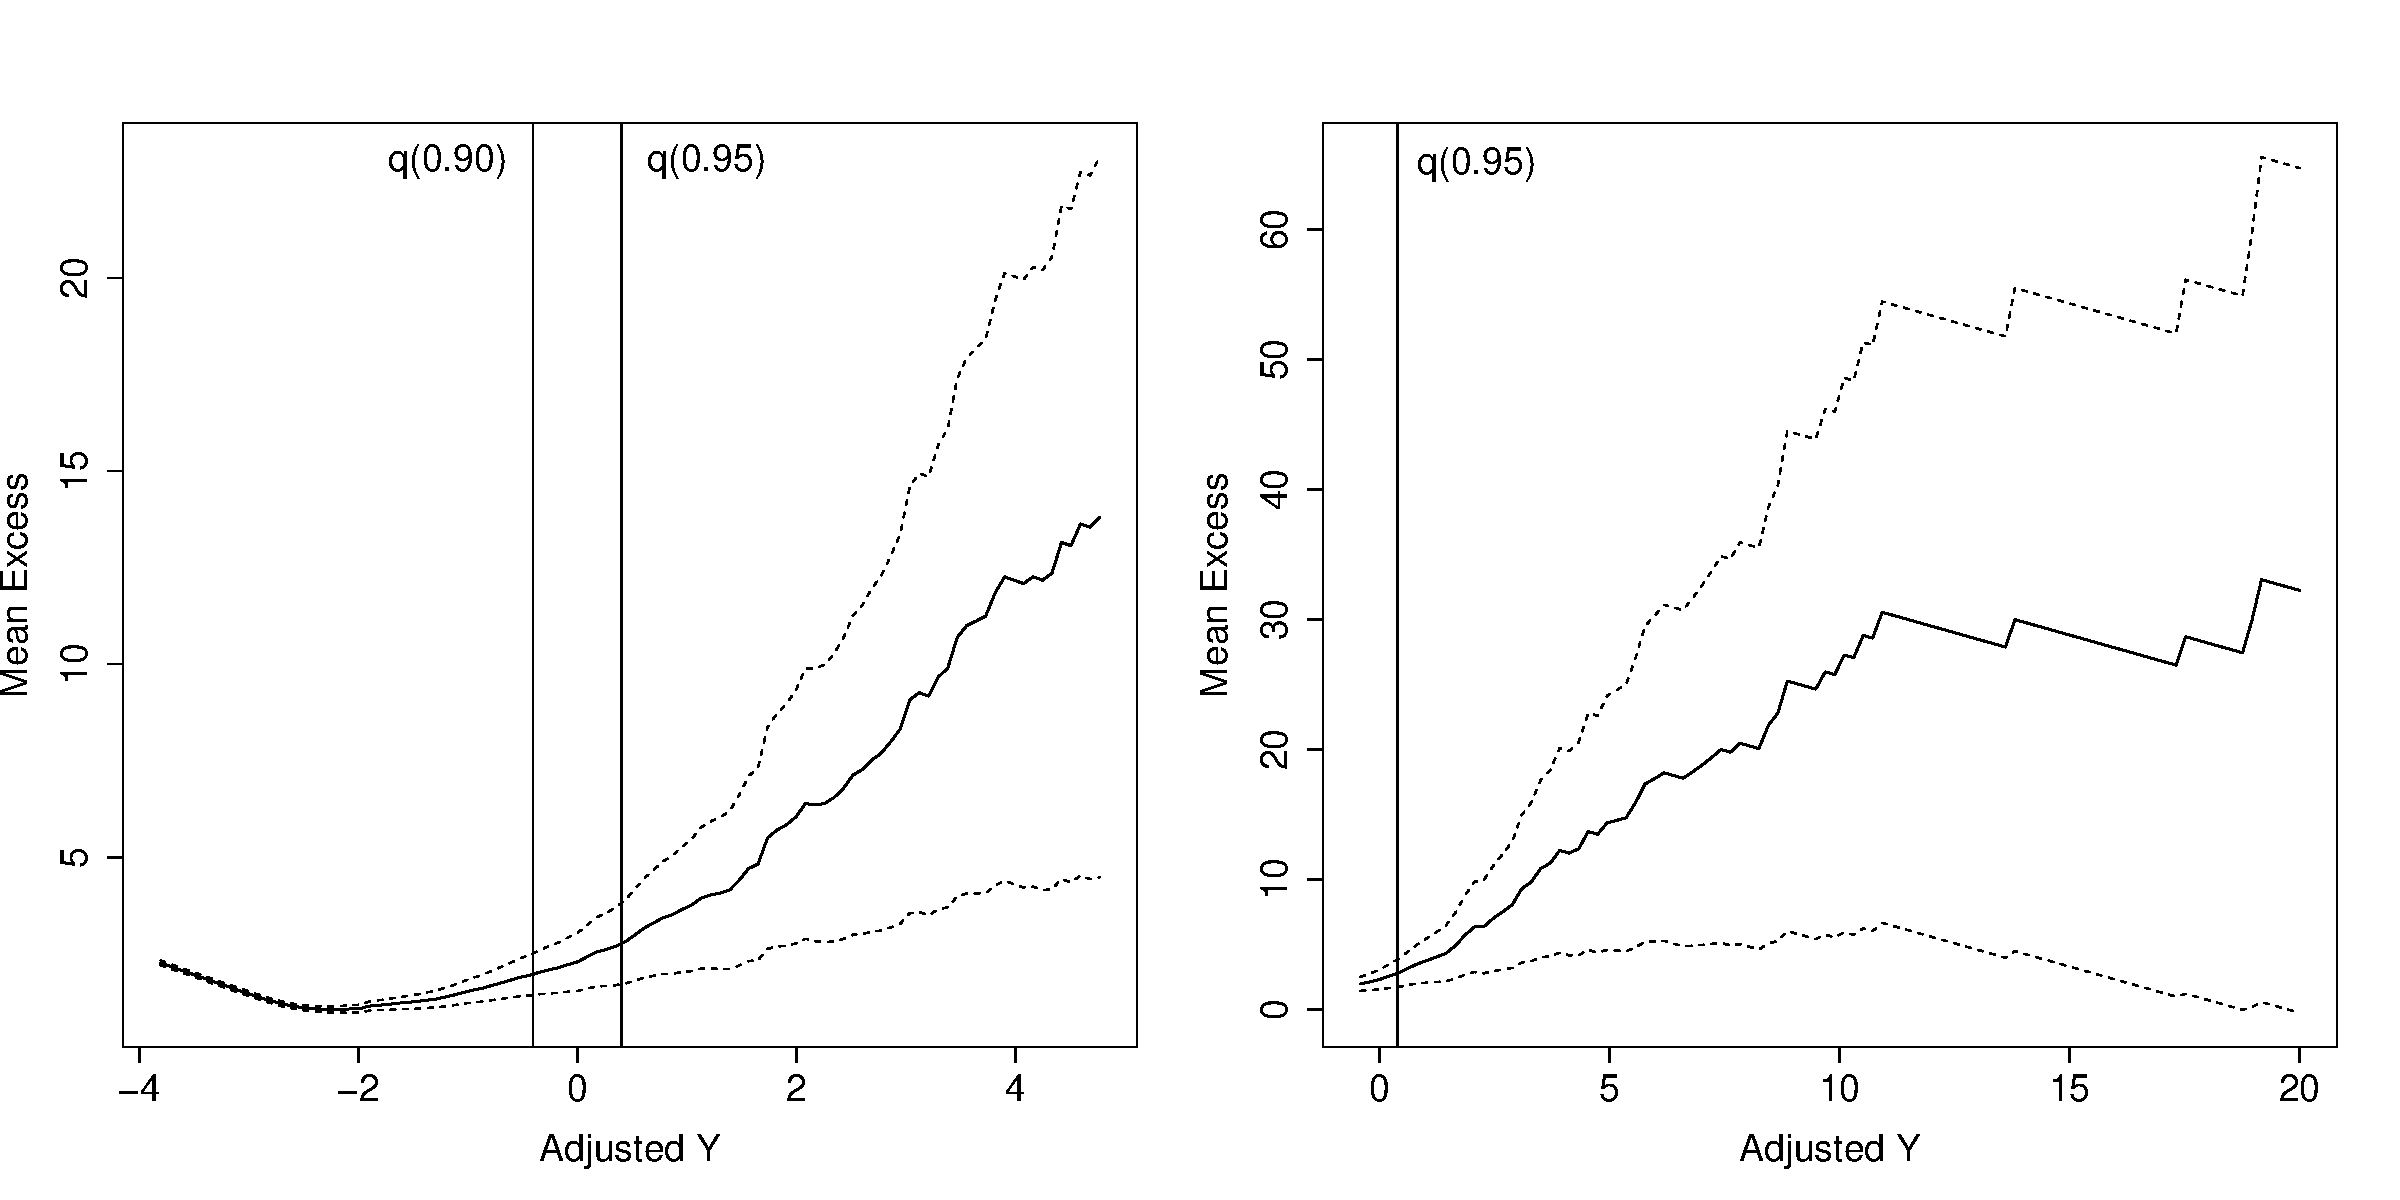
\includegraphics[width = \linewidth]{plots/fire-mrl-plots.pdf}
%  \caption{Mean residual plot for the data pooled across counties after standardizing using the county's median and interquartile range. The two panels show different ranges on the x-axis and include a vertical line at the sample 95th percentile.}
%  \label{ebfig:mrlthresh}
%\end{figure}
%
%%\begin{figure}[htbp]
%%  \centering
%%  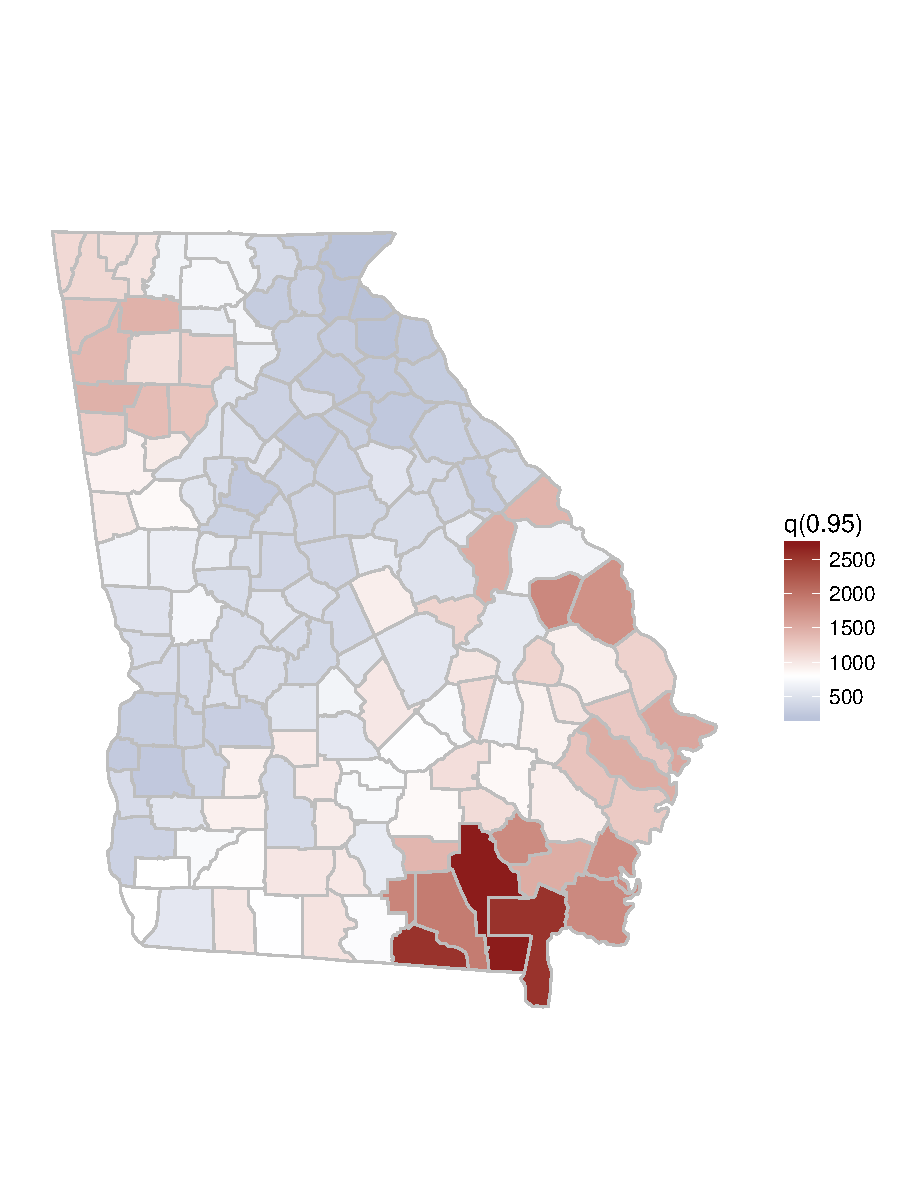
\includegraphics[width = 0.47\linewidth, trim = 0 10em 0 10em]{plots/fire-spatial-q95.pdf}
%%  \caption{Spatially smoothed threshold values for each county.}
%%  \label{fig:mrlthresh}
%%\end{figure}
%
%The empirical basis functions for the analysis can be used to help explore spatial dependence in the extremes.
%The first six EBFs for the wildfire data along with the cumulative sum of the contributions for $v_1, \ldots, v_{25}$ are given in \fref{ebfig:fire-ebfpanel}.
%\begin{figure}[htbp] % markdown/fire-analysis/basis-functions.R
%  \centering
%  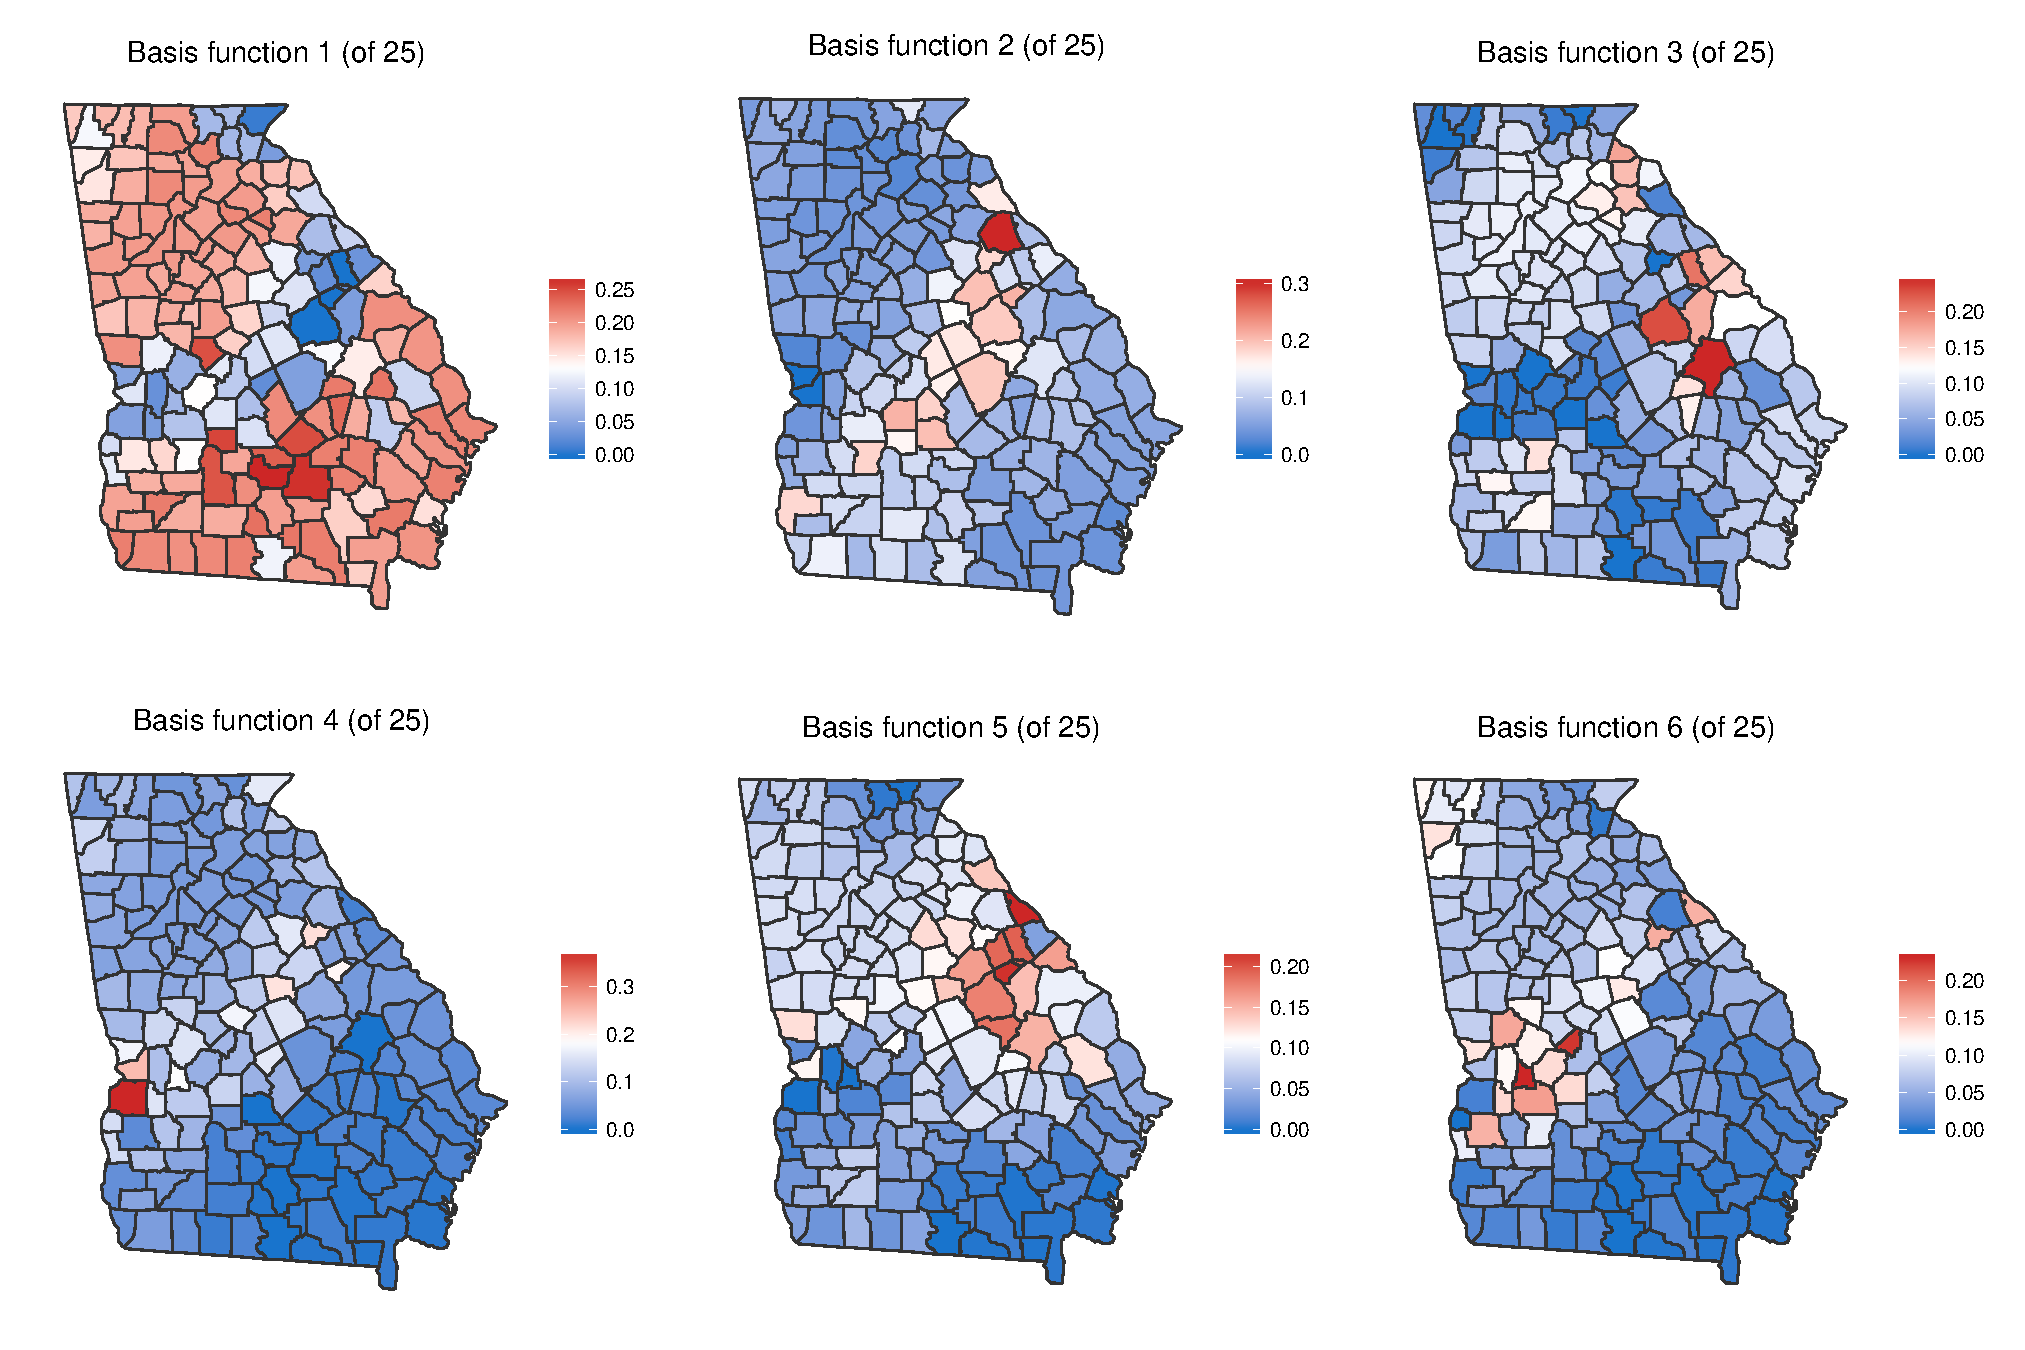
\includegraphics[width=\linewidth]{plots/fire-ebf-panel.pdf}\\
%  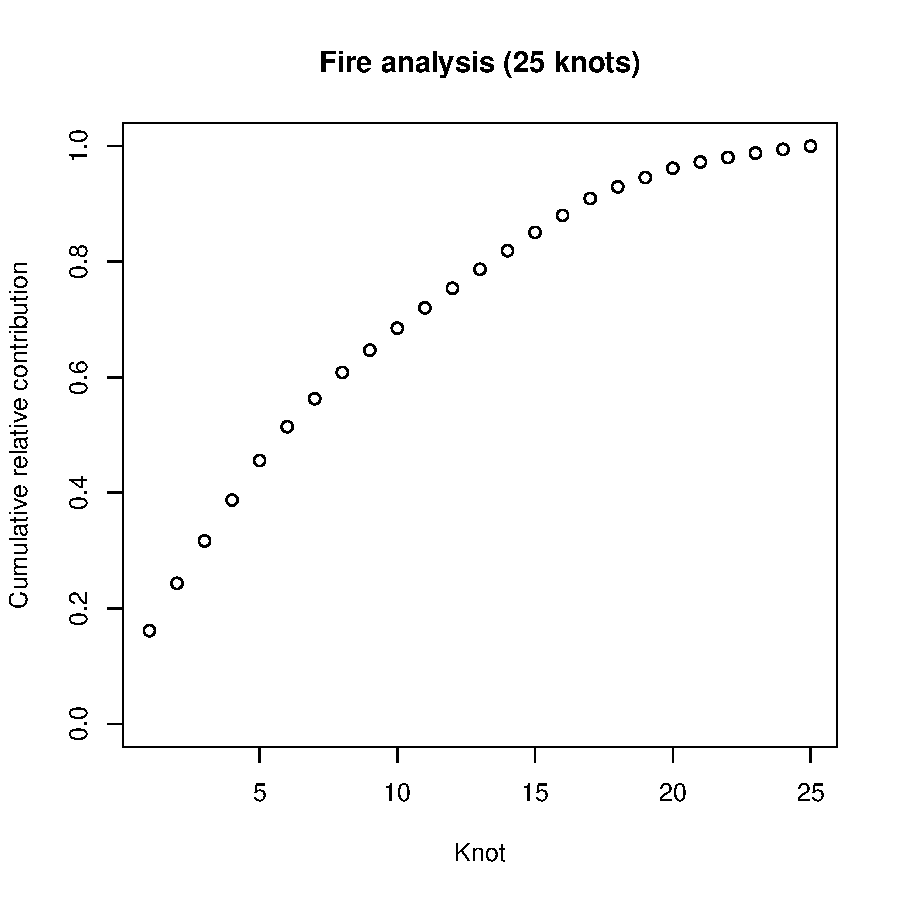
\includegraphics[width=0.45\linewidth]{plots/firev-25.pdf}
%  \caption{First six EBFs for the Georgia fire data and the cumulative sum of contributions $v_1, \ldots, v_{25}$.}
%  \label{ebfig:fire-ebfpanel}
%\end{figure}
%The first EBF roughly separates the Southeastern Plains (blue) from the coastal region in the southeast and mountains regions in the northeast (red).
%The remaining EBFs further partition the plains.
%As a comparison, we provide the first six principal components of the fire data along with the cumulative sum of the first 25 eigenvalues in \aref{eba:pca}.
%
%Given the basis function estimates, we run the MCMC for 35,000 iterations using a burnin period of 25,000 iterations.
%We consider models fit with both EBF and GSK, and fit the model using $L = 5, 10, \ldots, 40$.
%Timings for each setting of $L$ for 1,000 iterations are given in \tref{ebtbl:fire-scores}.
%These timings come from a single core of an Intel Core i7-5820K Haswell-E processor, using the OpenBLAS optimized BLAS library (\url{http://www.openblas.net}).
%
%\subsection{Results for fire analysis}\label{ebs:results-fire}
%
%We use 10-fold cross-validation to assess the predictive performance of a model.
%For each method, we randomly select 90\% of the observations across counties and years to be used as a training set to fit the model.
%The remaining 10\% of sites and years are withheld for testing model predictions.
%To assess the predictions for the test set, we use quantile scores and Brier scores \citep{Gneiting2007}.
%The quantile score (QS) for quantile level $q^*$ is given by \mbox{$2 \{I[Y(\bs) > \hat{q}(\bs)] - q^*]\}\{\hat{q}(\bs) - Y(\bs)\}$} where $\hat{q}(\bs)$ is the estimated $q^*$th quantile at site $\bs$, and $I[\cdot]$ is an indicator function.
%The Brier score (BS) for predicting an exceedance of a level $c$ at site $\bs$ is given by \mbox{$\{I[Y(\bs) > c] - \hat{P}[Y(\bs) > c]\}^2$}.
%For both of these methods, a lower score indicates a better fit.
%The Brier and quantile scores for the fire analysis are given in \tref{ebtbl:fire-scores}. %, and a plot of the scores are given in \fref{ebfig:fire-bsqs}.
%For the data, the BS and QS are fairly similar for all number of basis functions and the EBF versus GSK.
%This is perhaps due to the spatial variation in the marginal distribution explaining most of the spatial variation.
%In fact, using the EBFs, the estimate of residual dependence for the fire data is $\hat{\alpha} = 0.861$ ($\alpha = 1$ is residual independence).
%
%\begin{table}[htbp]
%\caption{Average Brier scores ($\times 100$), average quantile scores for $q(0.95)$ and $q(0.99)$, and time (in minutes) for 1,000 iterations for fire analysis.}
%\label{ebtbl:fire-scores}
%\centering
%  \begin{tabular}{llcrrcrrcc}
%  \toprule
%  & & \phantom{ab} & \multicolumn{2}{c}{Brier Scores ($\times 100$)} & \phantom{abc} & \multicolumn{2}{c}{Quantile Scores} & \phantom{ab} & \\
%  \cmidrule{4-5} \cmidrule{7-8}
%  & Process && $q(0.95)$ & $q(0.99)$ && $q(0.95)$ & $q(0.99)$ && Time\\
%  \midrule
%  L = 5  & EBF && 4.269 & 1.653 && 107.904 & 67.345 && 1.16\\
%         & GSK && 4.244 & 1.644 && 103.822 & 64.046 && 1.18\\
%  \midrule
%  L = 10 & EBF && 4.328 & 1.675 && 107.075 & 66.300 && 1.56\\
%         & GSK && 4.170 & 1.665 && 104.214 & 64.589 && 1.47\\
%  \midrule
%  L = 15 & EBF && 4.330 & 1.690 && 108.381 & 67.671 && 1.86\\
%         & GSK && 4.214 & 1.654 && 104.490 & 65.201 && 1.83\\
%  \midrule
%  L = 20 & EBF && 4.346 & 1.697 && 107.389 & 66.957 && 2.18\\
%         & GSK && 4.174 & 1.646 && 104.671 & 65.430 && 2.20\\
%  \midrule
%  L = 25 & EBF && 4.263 & 1.650 && 106.656 & 64.913 && 2.54\\
%         & GSK && 4.216 & 1.661 && 104.208 & 64.468 && 2.55\\
%  \midrule
%  L = 30 & EBF && 4.328 & 1.678 && 106.265 & 64.674 && 2.90\\
%         & GSK && 4.228 & 1.660 && 104.143 & 64.443 && 2.92\\
%  \midrule
%  L = 35 & EBF && 4.329 & 1.671 && 106.817 & 65.002 && 3.29\\
%         & GSK && 4.256 & 1.663 && 105.016 & 64.920 && 3.32\\
%  \midrule
%  L = 40 & EBF && 4.284 & 1.653 && 106.621 & 64.753 && 3.70\\
%         & GSK && 4.233 & 1.666 && 105.301 & 64.932 && 3.56\\
%  \bottomrule
%  \end{tabular}
%\end{table}
%
%% \begin{figure}[htbp]  % markdown/fire-analysis/combine-tables.R
%%   \centering
%%   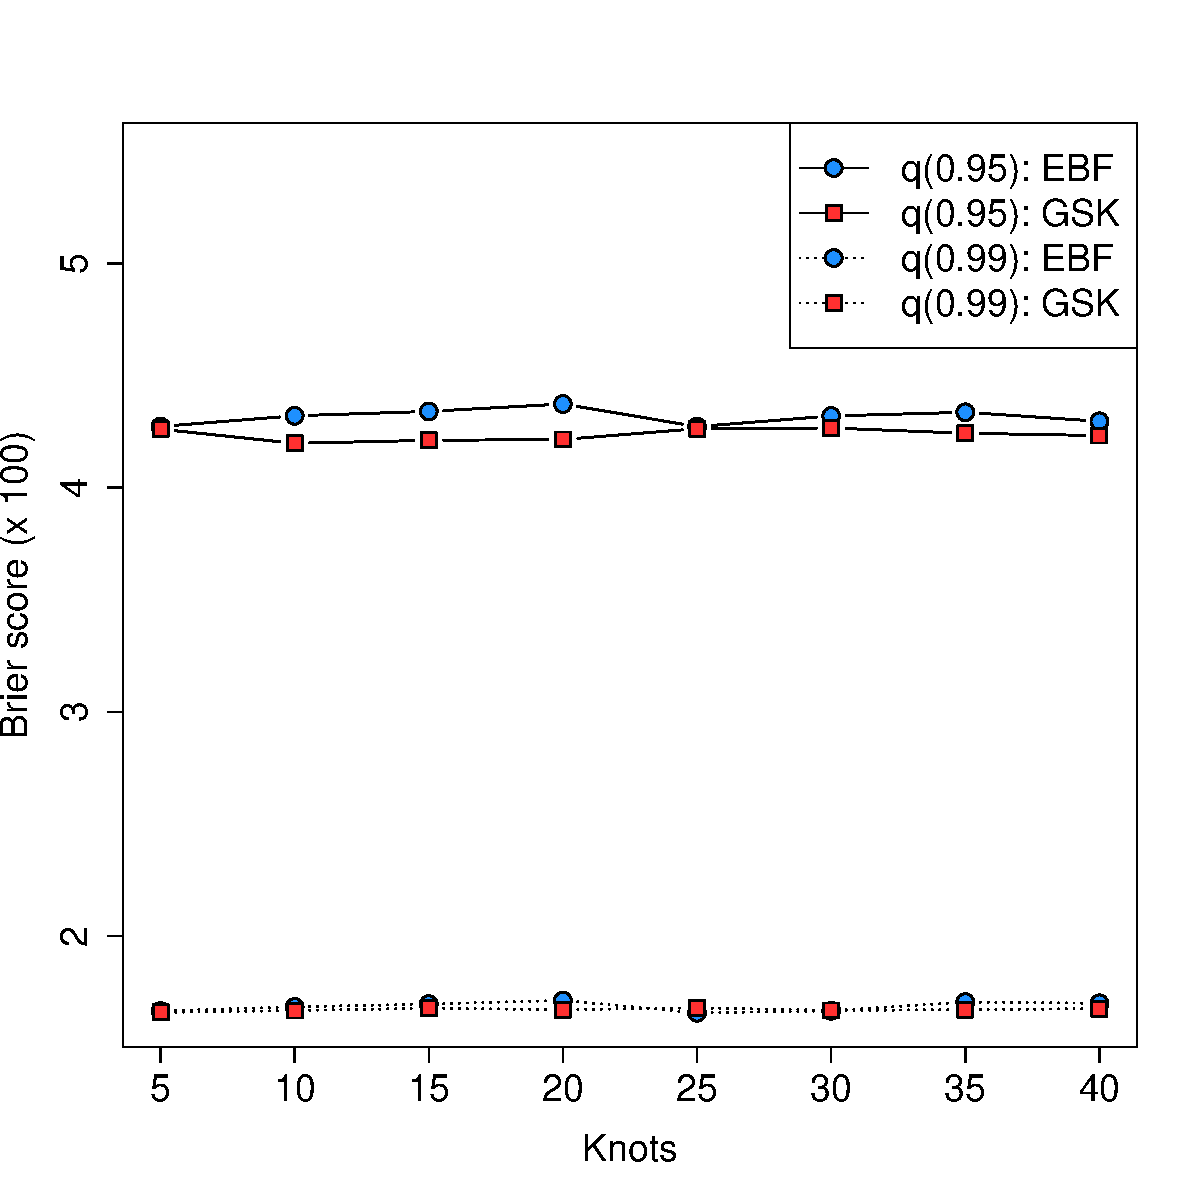
\includegraphics[width=0.49\linewidth]{plots/fire-bs.pdf}
%%   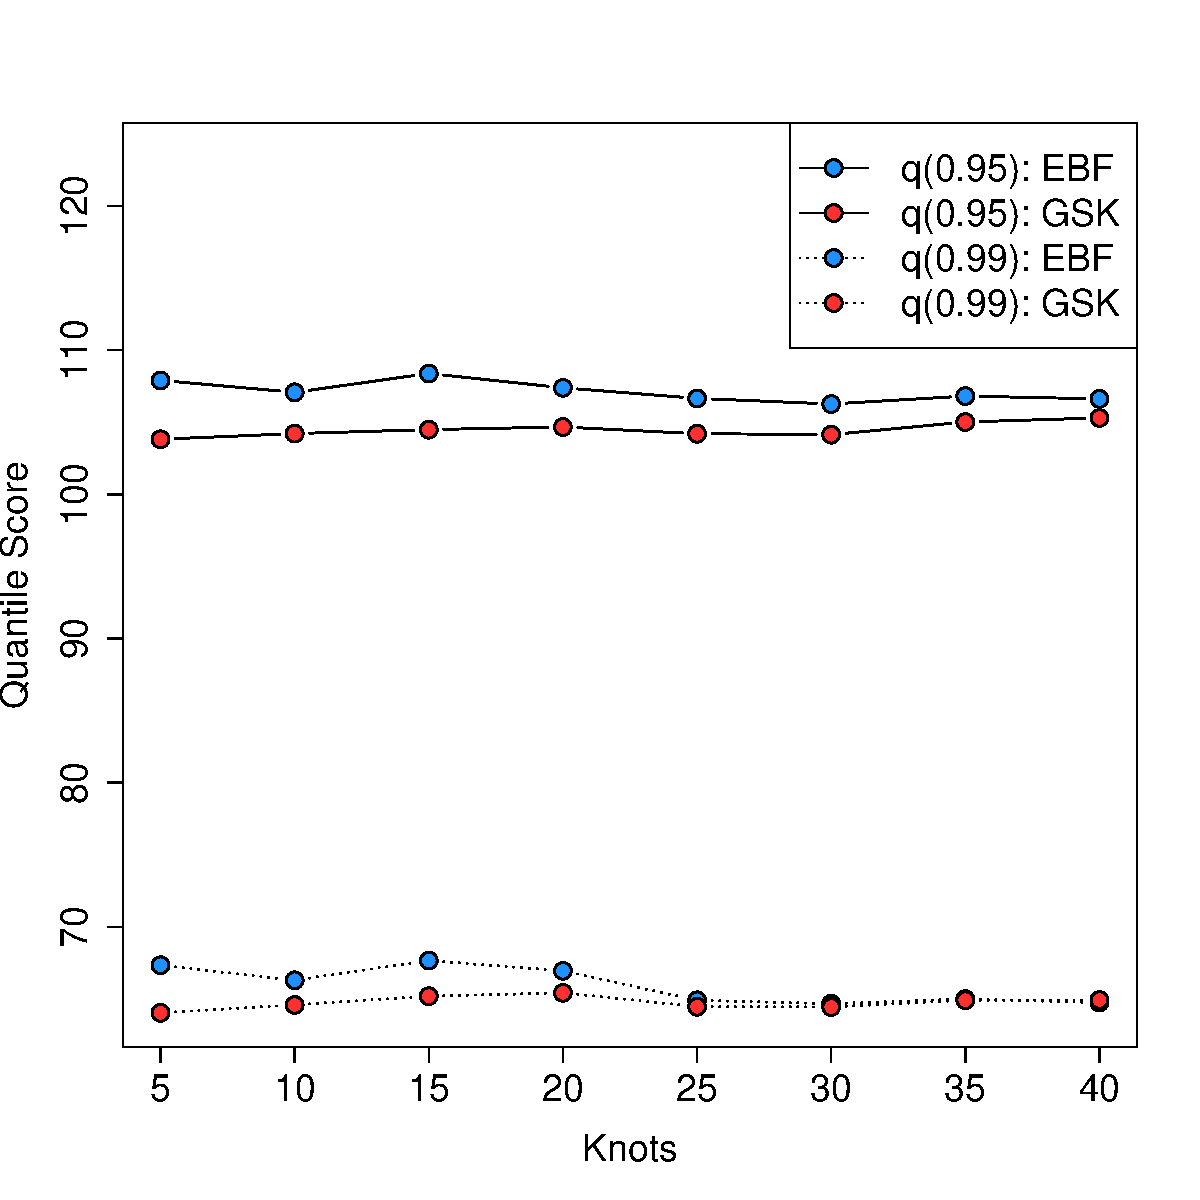
\includegraphics[width=0.49\linewidth]{plots/fire-qs.pdf}
%%   \caption{Brier scores (left) and quantile scores (right) for $q(0.95)$ and $q(0.99)$ to compare EBF and GSK analysis of Georgia fire data.}
%%   \label{ebfig:fire-bsqs}
%% \end{figure}
%
%% \begin{figure}[htbp]  % markdown/fire-analysis/posterior_map.R
%%   \centering
%%   \includegraphics[width=\linewidth]{plots/fire-ebf-post-betatime.pdf}
%%   \caption{Posterior mean of $\beta_{1, \text{time}}$ (left) and $\beta_{2, \text{time}}$ (right) for fire data using EBF.}
%%   \label{ebfig:fire-ebfpostbeta1}
%% \end{figure}
%
%% \begin{figure}[htbp]  % markdown/fire-analysis/posterior_map.R
%%   \centering
%%   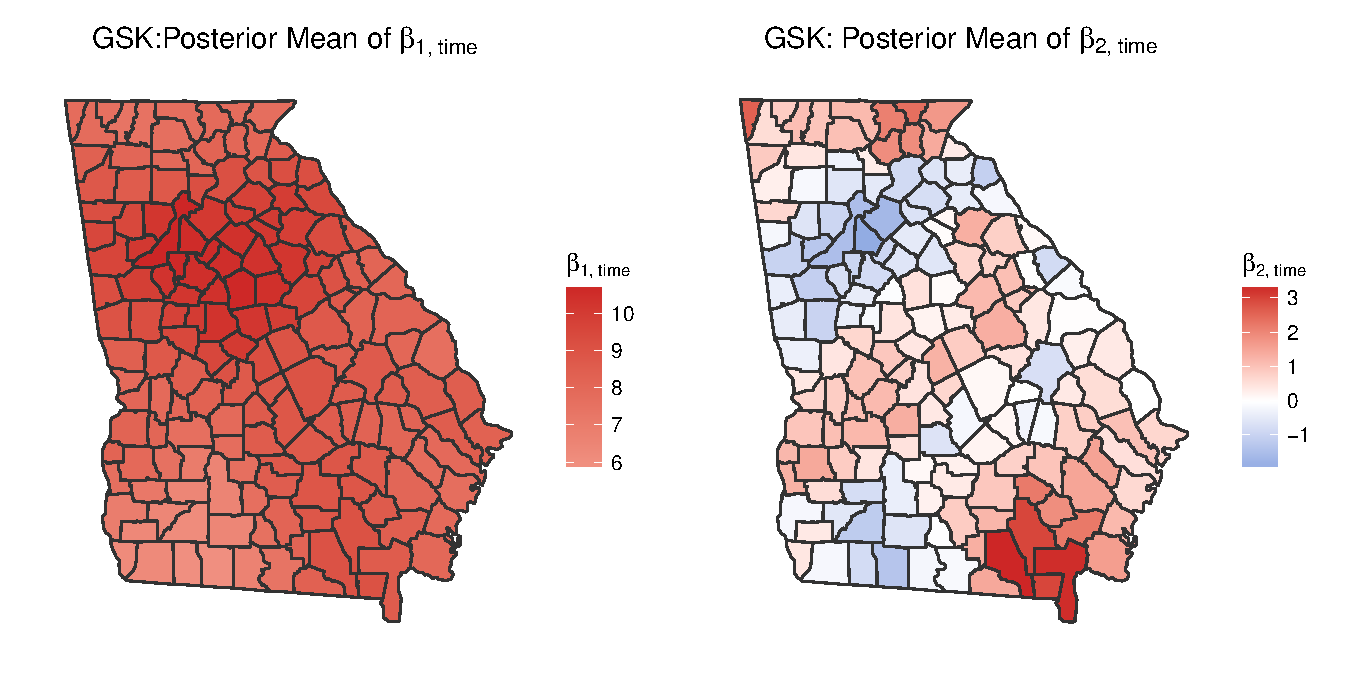
\includegraphics[width=\linewidth]{plots/fire-gsk-post-betatime.pdf}
%%   \caption{Posterior mean of $\beta_{1, \text{time}}$ (left) and $\beta_{2, \text{time}}$ (right) for fire data using GSK.}
%%   \label{ebfig:fire-gskpostbeta1}
%% \end{figure}
%
%% \begin{figure}[htbp]  % markdown/fire-analysis/posterior_map.R
%%   \centering
%%   \includegraphics[width=\linewidth]{plots/fire-ebf-post-betatimepos.pdf}
%%   \caption{Posterior P$(\beta_{1, \text{time}} > 0)$ (left) and P$(\beta_{2, \text{time}} > 0)$ (right) for fire data using EBF.}
%%   \label{ebfig:fire-ebfpostbeta1pos}
%% \end{figure}
%
%% \begin{figure}[htbp]  % markdown/fire-analysis/posterior_map.R
%%   \centering
%%   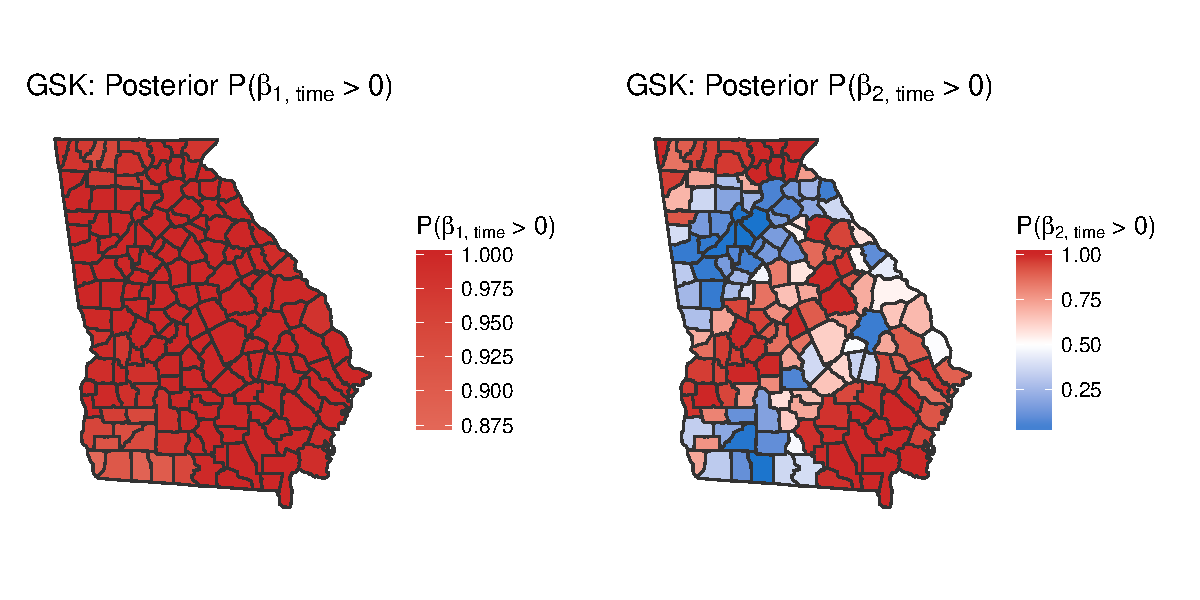
\includegraphics[width=\linewidth]{plots/fire-gsk-post-betatimepos.pdf}
%%   \caption{Posterior P$(\beta_{1, \text{time}} > 0)$ (left) and P$(\beta_{2, \text{time}} > 0)$ (right) for fire data using GSK.}
%%   \label{ebfig:fire-gskpostbeta1pos}
%% \end{figure}
%
%Based on the cross-validation results, we run a full analysis using all of the data with $L = 25$.
%Despite the GSK model having slightly smaller BS and QS values, we use the EBF method.
%\fref{ebfig:fire-ebf-postpanel} gives posterior summaries for three quantities of interest.
%We provide maps of the linear time trend in the GEV location ($\beta_{1, \text{time}, i}$), and GEV log scale  ($\beta_{2, \text{time}, i}$)  and a map of \mbox{$\Delta Q90_i = Q90_{i, 2014} - Q90_{i, 1965}$} the change in the mean of the posterior distribution of $Q90_{i, t}$ between $t_1 = 1965$ and $t_2 = 2014$.
%We also provide maps of the posterior probability that each of the three terms is positive.
%
%We construct the posterior distribution of the the estimated 90th quantile $Q90_{i, t}$ using the GEV parameters as follows.
%Let $Q90_{i, t}^{(j)}$ be the estimated 90th quantile at site $i$ for time $t$ at iteration $j$.
%We first compute
%\begin{align}
%  \mu_{i, t}^{(j)} &= \beta_{1, \text{int}, i}^{(j)} + \beta_{1, \text{time}, i}^{(j)} t \\
%  \log\left(\sigma_{i, t}^{(j)}\right) &= \beta_{2, \text{int}, i}^{(j)} + \beta_{2, \text{time}, i}^{(j)} t. \nonumber
%\end{align}
%Let $Q90_{i, t}^{(j)} = \mu_{i, t}^{(j)} + \sigma_{i, t}^{(j)} F^{-1}\left(0.90, \xi^{(j)}\right)$ where $F^{-1}(q, \xi)$ is the inverse distribution function of the GEV$(1, 1, \xi)$ distribution evaluated at the $q$th quantile.
%Finally, let $Q90_{i, t}$ be posterior mean of $Q90_{i, t}^{(j)}$.
%To obtain the posterior probability of seeing an increase over time, we take the posterior distributions of each parameter of interest at the two time points.
%Consider two time points $t_1 < t_2$.
%Let $\varphi_t^{(j)}$ be the parameter of interest at iteration $j$ and time $t$.
%We then take the posterior mean of $I\left[\varphi_{t_2}^{(j)} > \varphi_{t_1}^{(j)}\right]$, for the posterior probability of seeing an increase in $\varphi$ from time $t_1$ to $t_2$.
%
%These results suggest that there has been a slight increase in the amount of acres burned over time.
%When looking at the variability of the acres burned over time, we see some patterns that generally correspond to landcover in Georgia (see \url{http://narsal.uga.edu/} for landcover maps).
%In the high intensity urban areas (e.g. the Piedmont region) and croplands, we see a decrease in variability as well as very low P$[\Delta Q90 > 0]$.
%However, in the more forested areas (e.g. Blue Ridge mountains, Okefenokee Swamp), we see increased variability over time as well as a high P$[\Delta Q90 > 0]$.
%This suggests that the 10-year return level for wildfires in regions with larger tree cover is increasing over time which corresponds with increased drought and higher temperatures.
%
%\begin{figure}[htbp]  % markdown/fire-analysis/posterior_map.R
%  \centering
%  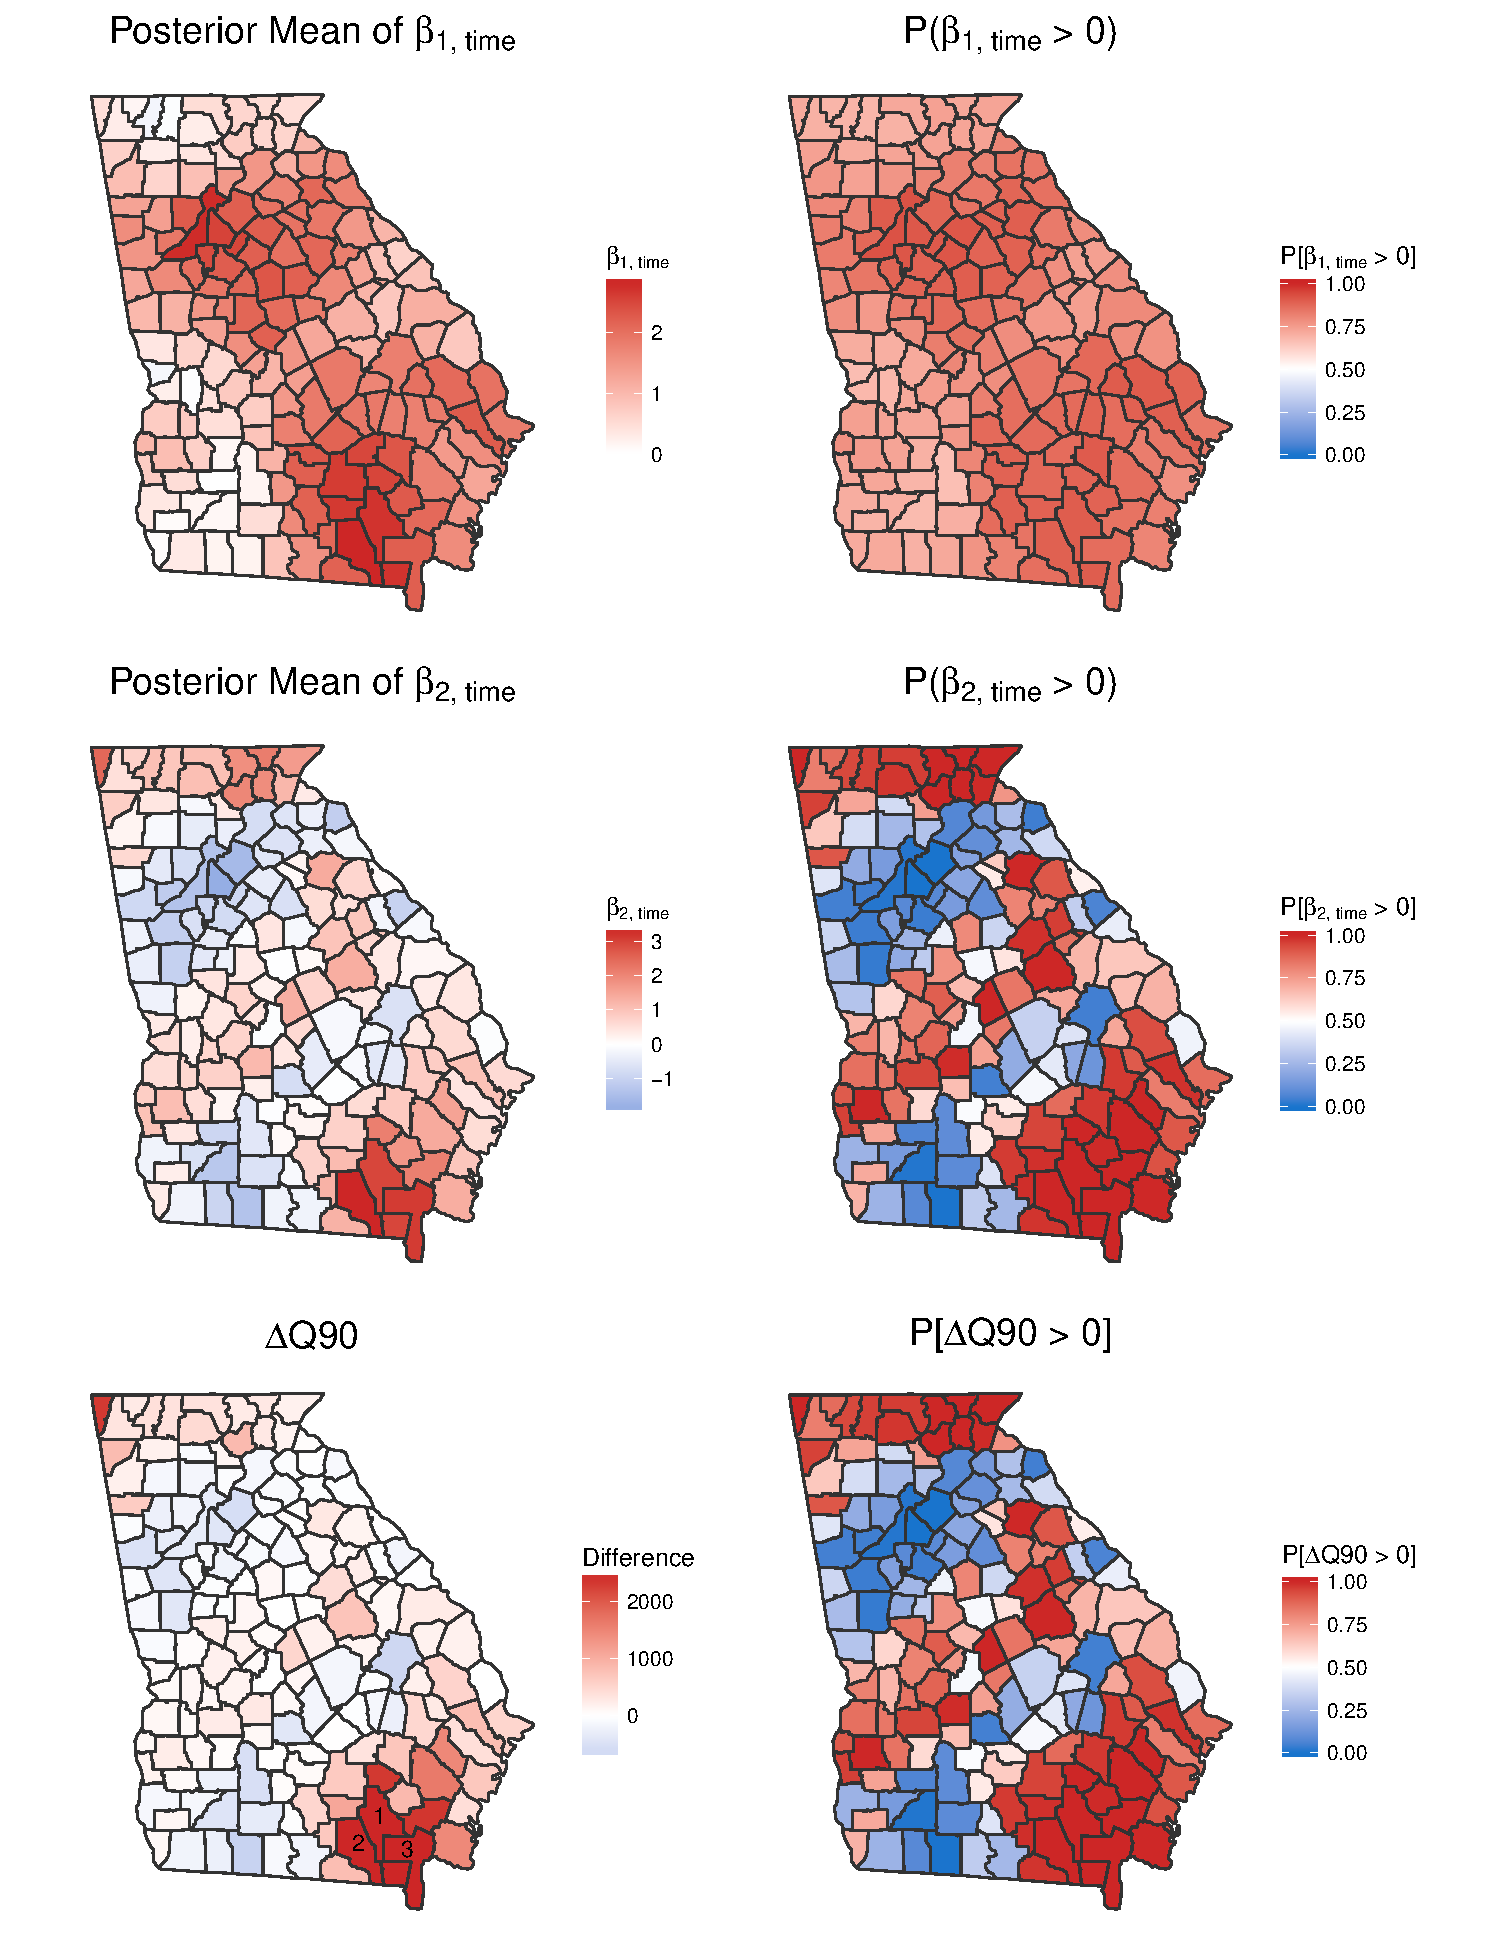
\includegraphics[height=0.9\textheight]{plots/fire-ebf-postpanel.pdf}
%  \caption{Posterior mean of $\beta_{1, \text{time}}$ (top left), posterior mean of $\beta_{2, \text{time}}$ (middle left), estimate of $\Delta Q90$ (bottom left), P$[\beta_{1, \text{time}} > 0]$ (top right), P$[\beta_{2, \text{time}} > 0]$ (middle right), and P$[\Delta Q90 > 0]$ for fire data using EBF. In three counties (labeled), $\Delta Q90 > 2500$: County 1 - Ware (11,109), County 2 - Clinch (7,128), and County 3 - Charlton (6,545)}
%  \label{ebfig:fire-ebf-postpanel}
%\end{figure}
%
%% \begin{figure}  % markdown/fire-analysis/combine-tables.R
%%   \centering
%%   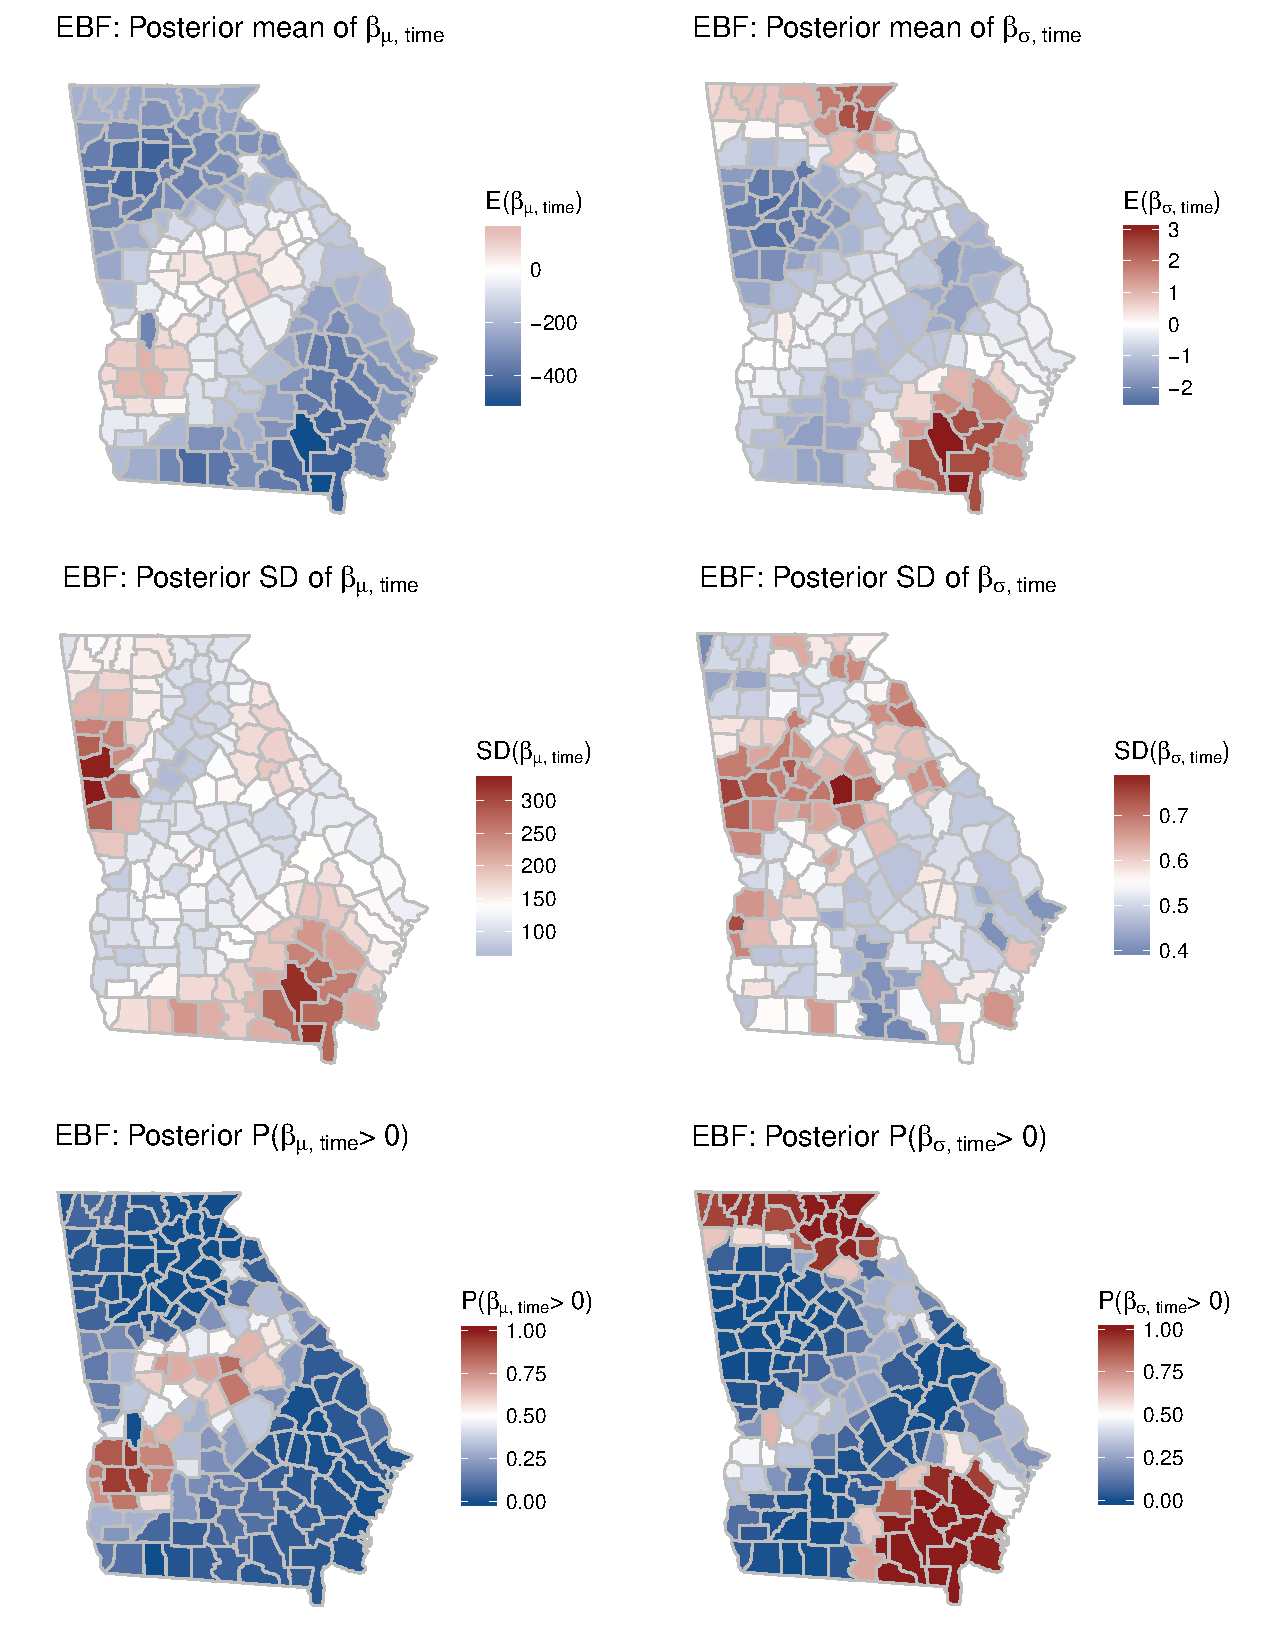
\includegraphics[width=\linewidth]{plots/ebf-post-betatime.pdf}
%%   \caption{Posterior summaries of $\beta_{\text{time}}$ when using EBF for the spatial process with $L = 35$.}
%%   \label{ebfig:ebfpost}
%% \end{figure}
%
%% \begin{figure}  % markdown/fire-analysis/combine-tables.R
%%   \centering
%%   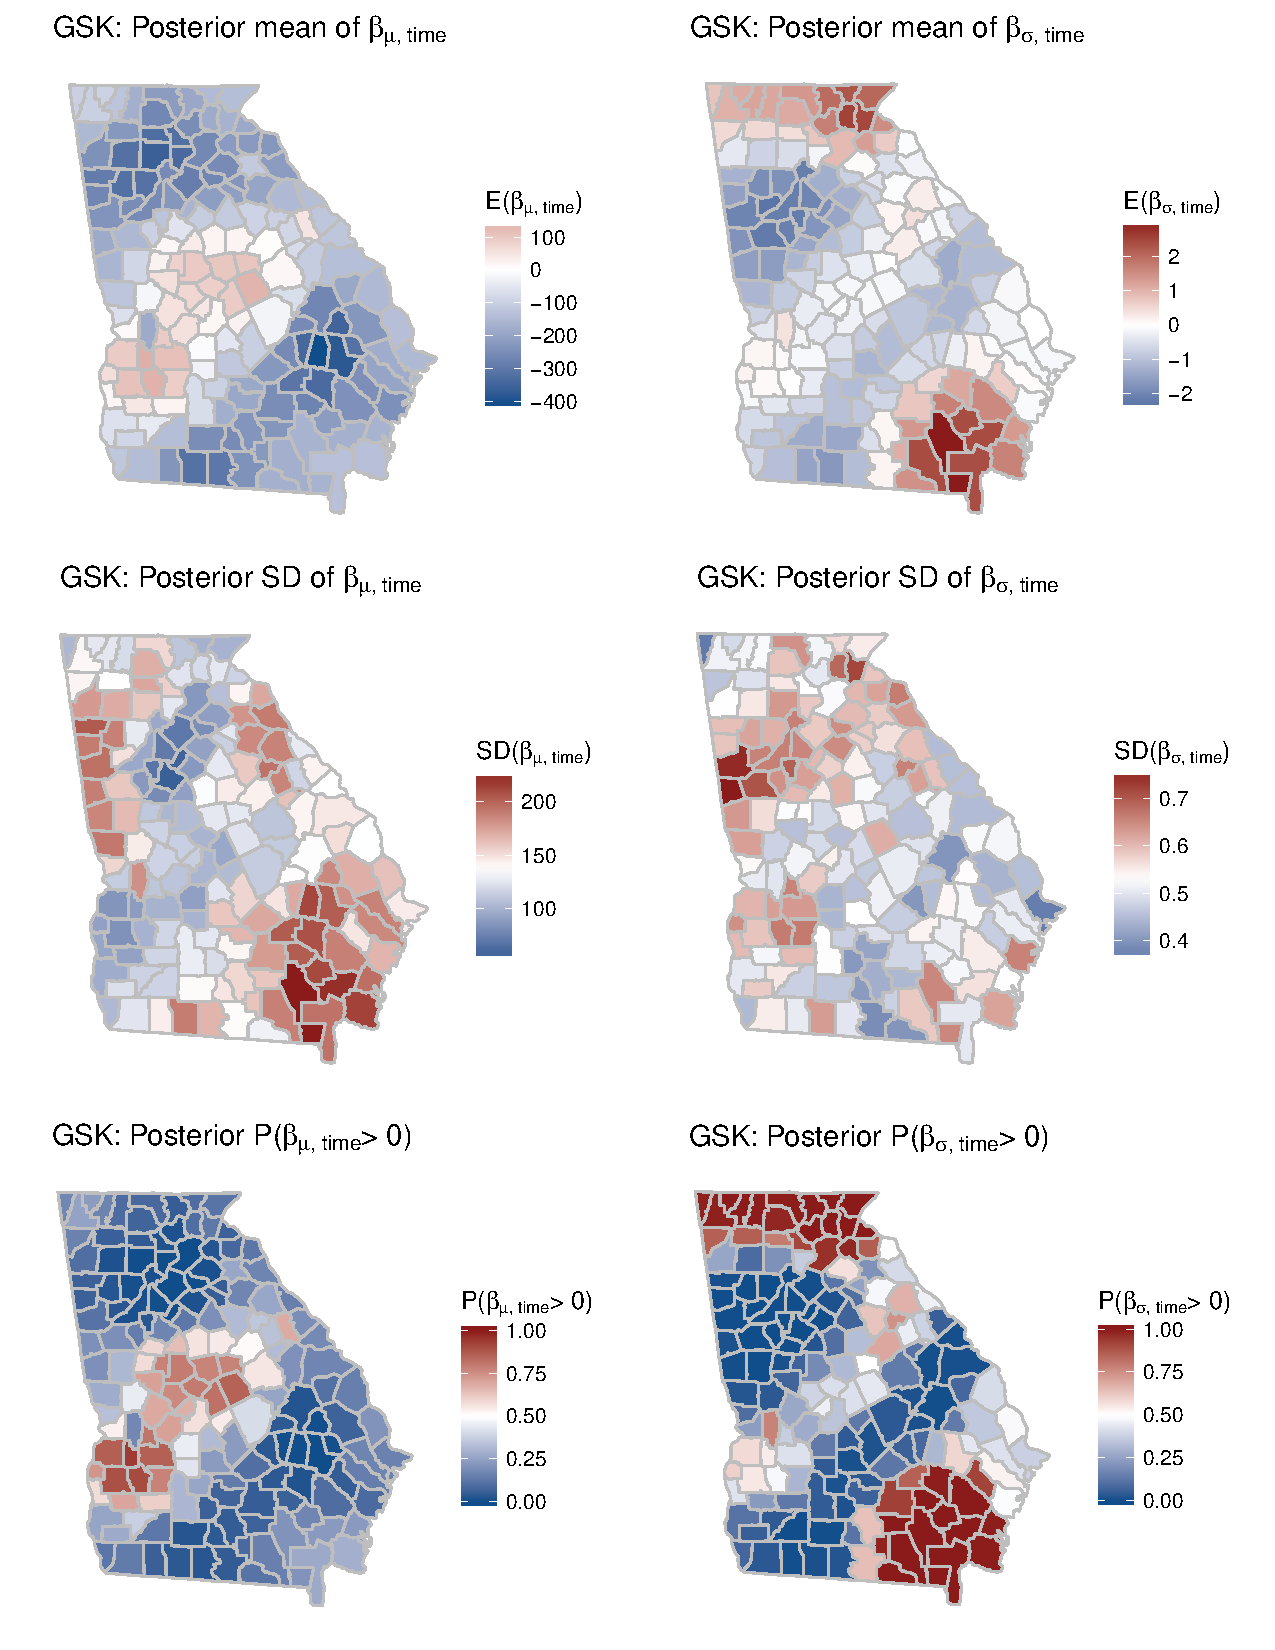
\includegraphics[width=\linewidth]{plots/gsk-post-betatime.pdf}
%%   \caption{Posterior summaries of $\beta_{\text{time}}$ when using GSK for the spatial process with $L = 35$.}
%%   \label{ebfig:gskpost}
%% \end{figure}
%
%% \begin{figure}  % markdown/fire-analysis/combine-tables.R
%%   \centering
%%   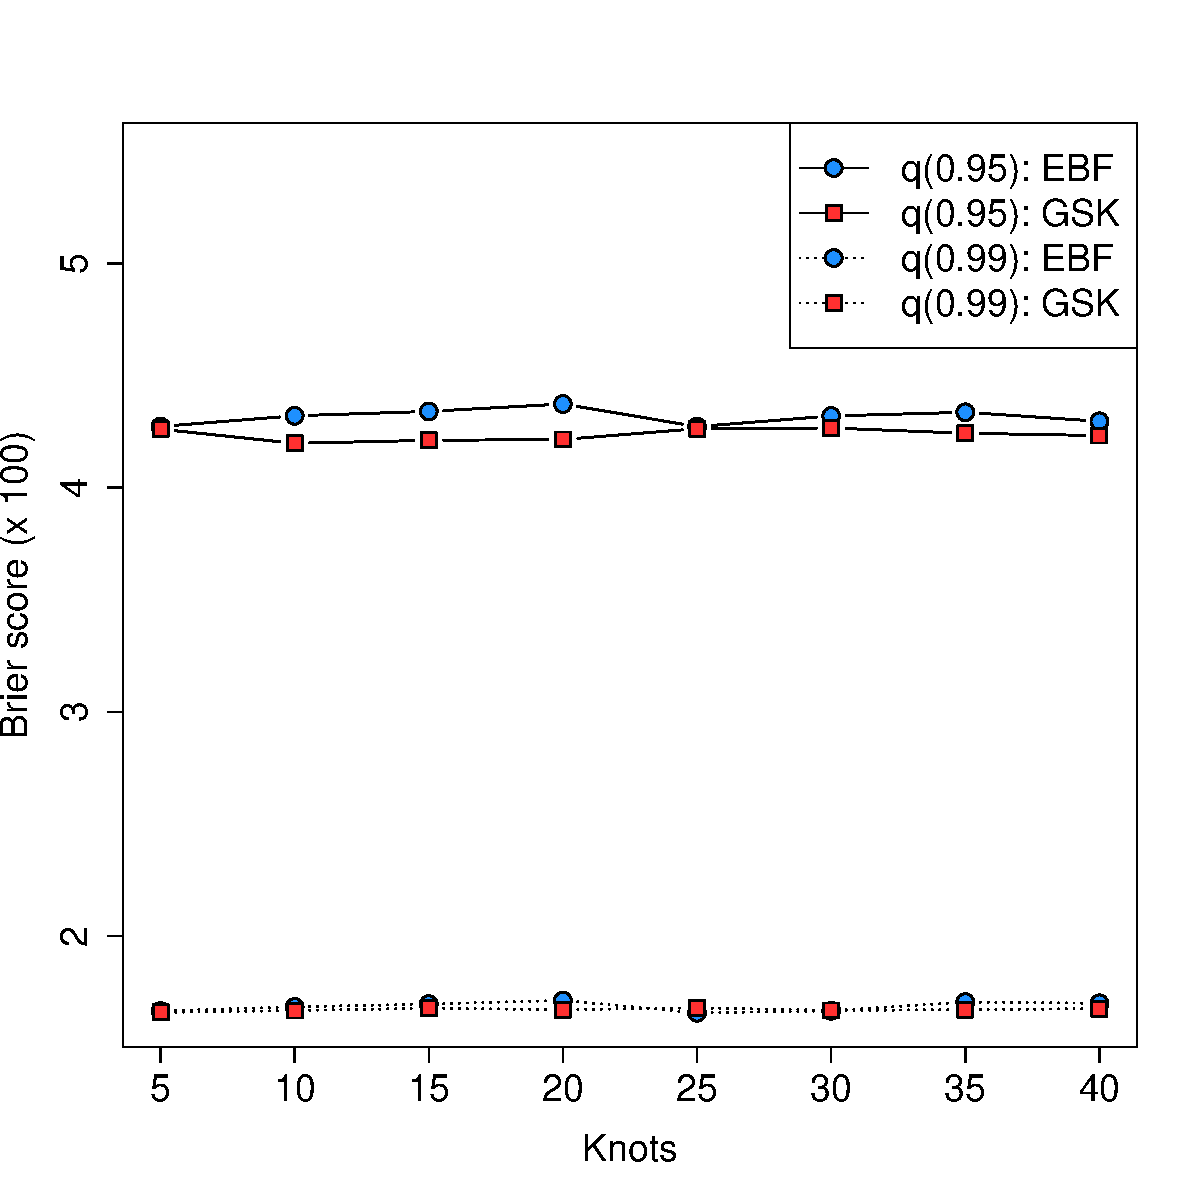
\includegraphics[width=0.47\linewidth]{plots/fire-bs}
%%   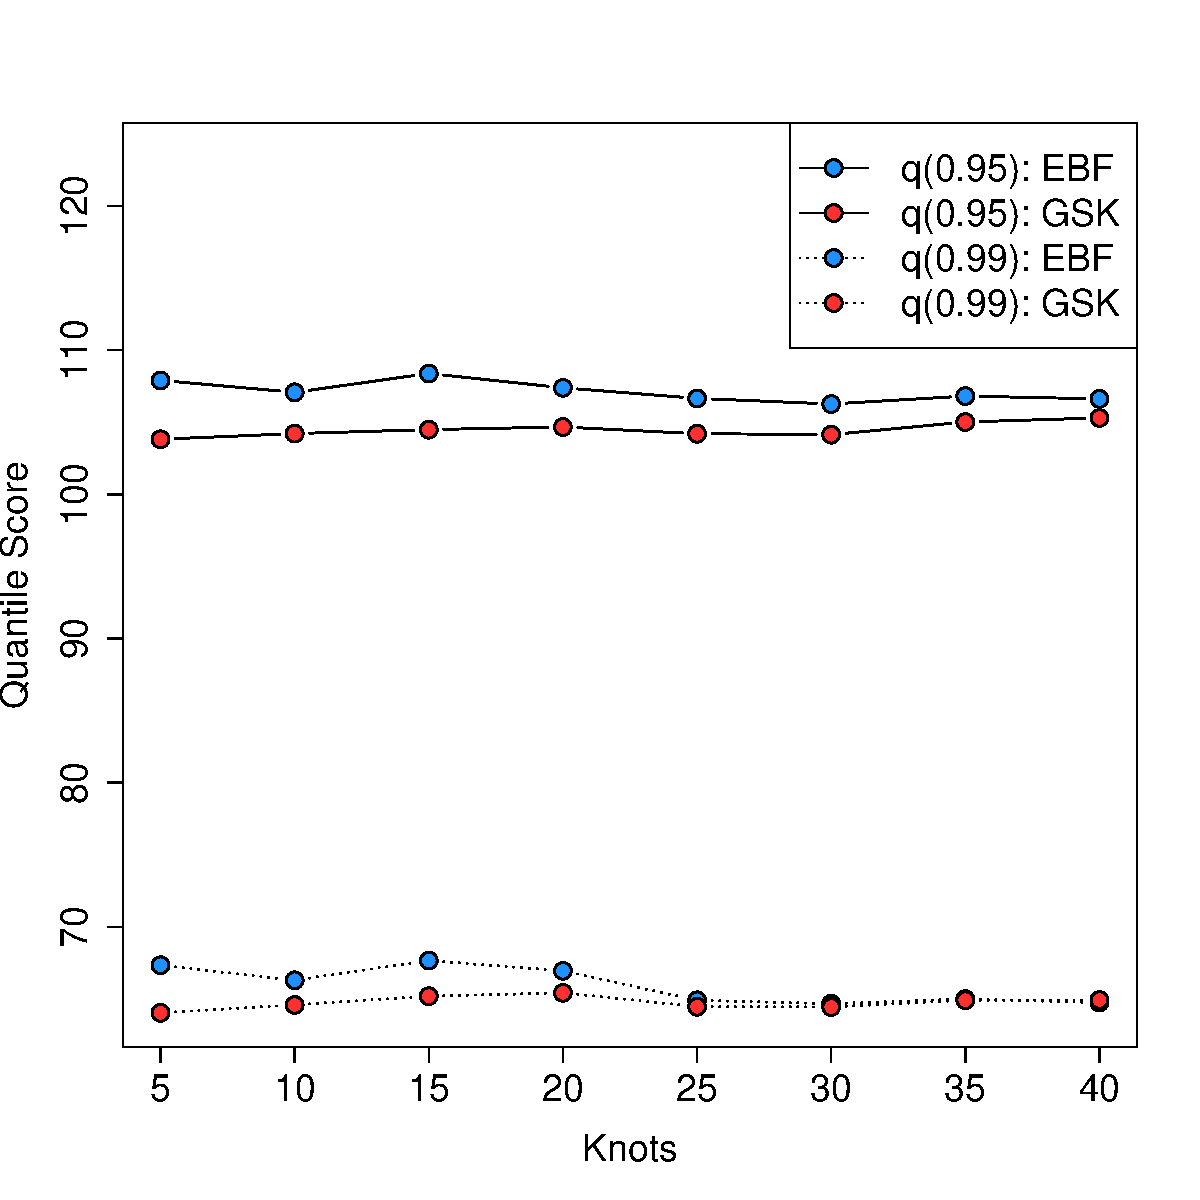
\includegraphics[width=0.47\linewidth]{plots/fire-qs}
%%   \caption{Average Brier score for exceeding q(0.95) and q(0.99) (left). Average Quantile score for exceeding q(0.95) and q(0.99) (right).}
%%   \label{fig:avgqscore}
%% \end{figure}
%
%% \begin{figure}  % markdown/fire-analysis/combine-tables.R
%%   \centering
%%   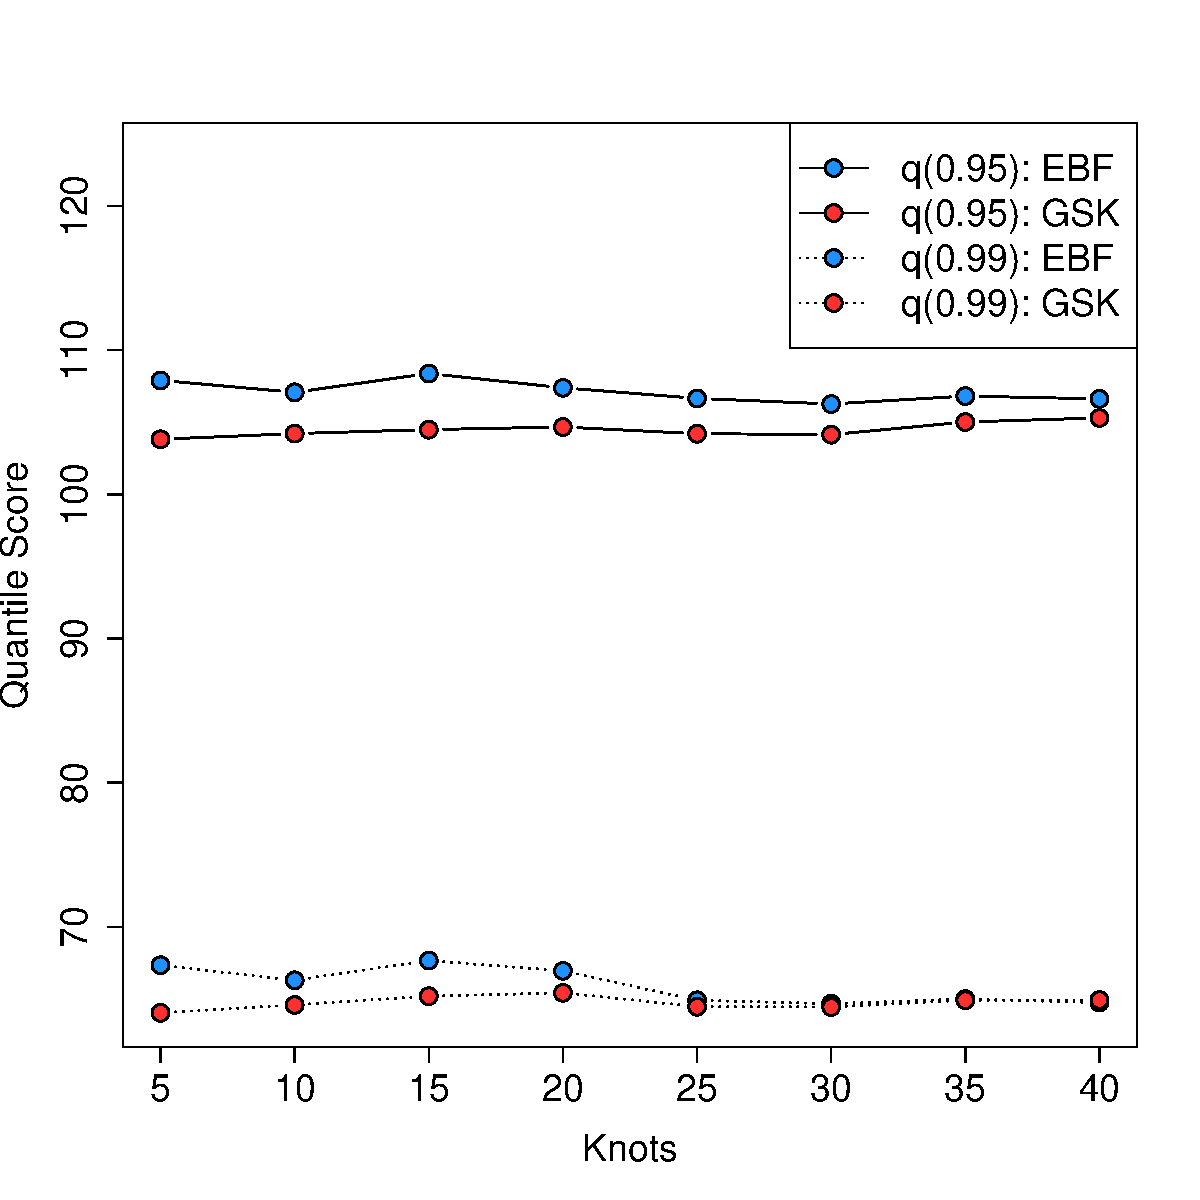
\includegraphics[width=\linewidth]{plots/fire-qs}
%%   \caption{Average quantile score for q(0.95) (left). Average quantile score for q(0.99) (right).}
%%   \label{fig:avgqscore}
%% \end{figure}
%
%% \begin{figure}  % markdown/fire-analysis/combine-tables.R
%%   \centering
%%   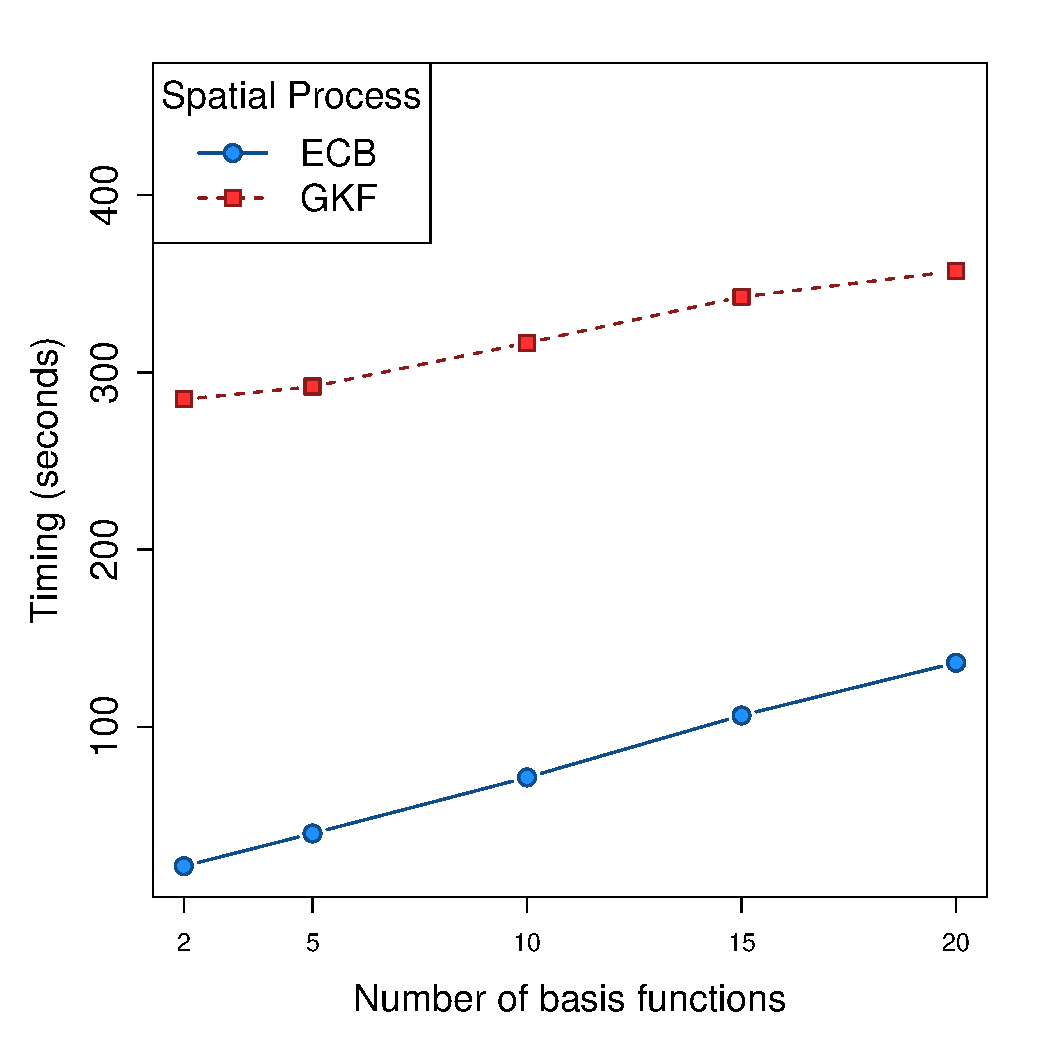
\includegraphics[width=0.47\linewidth]{plots/fire-timing}
%%   \caption{Timing comparison of basis functions to kernel functions for the spatial process (100 iterations)}
%%   \label{fig:timingcompare}
%% \end{figure}

\subsection{Analysis of annual precipitation}\label{ebs:precip}

We also conduct an analysis of the precipitation data presented in \citet{Reich2012}.
The data are climate model output from the North American Regional Climate Change Assessment Program (NARCCAP).
This data consists of $n_s = 697$ grid cells at a 50km resolution in the eastern US, and includes historical data (1969 -- 2000) as well as future conditions (2039 -- 2070).
Because the data are block maxima, we set $T = -\infty$.

\begin{figure}[htbp]  % markdown/precipitation/cv-setup.R
  \centering
  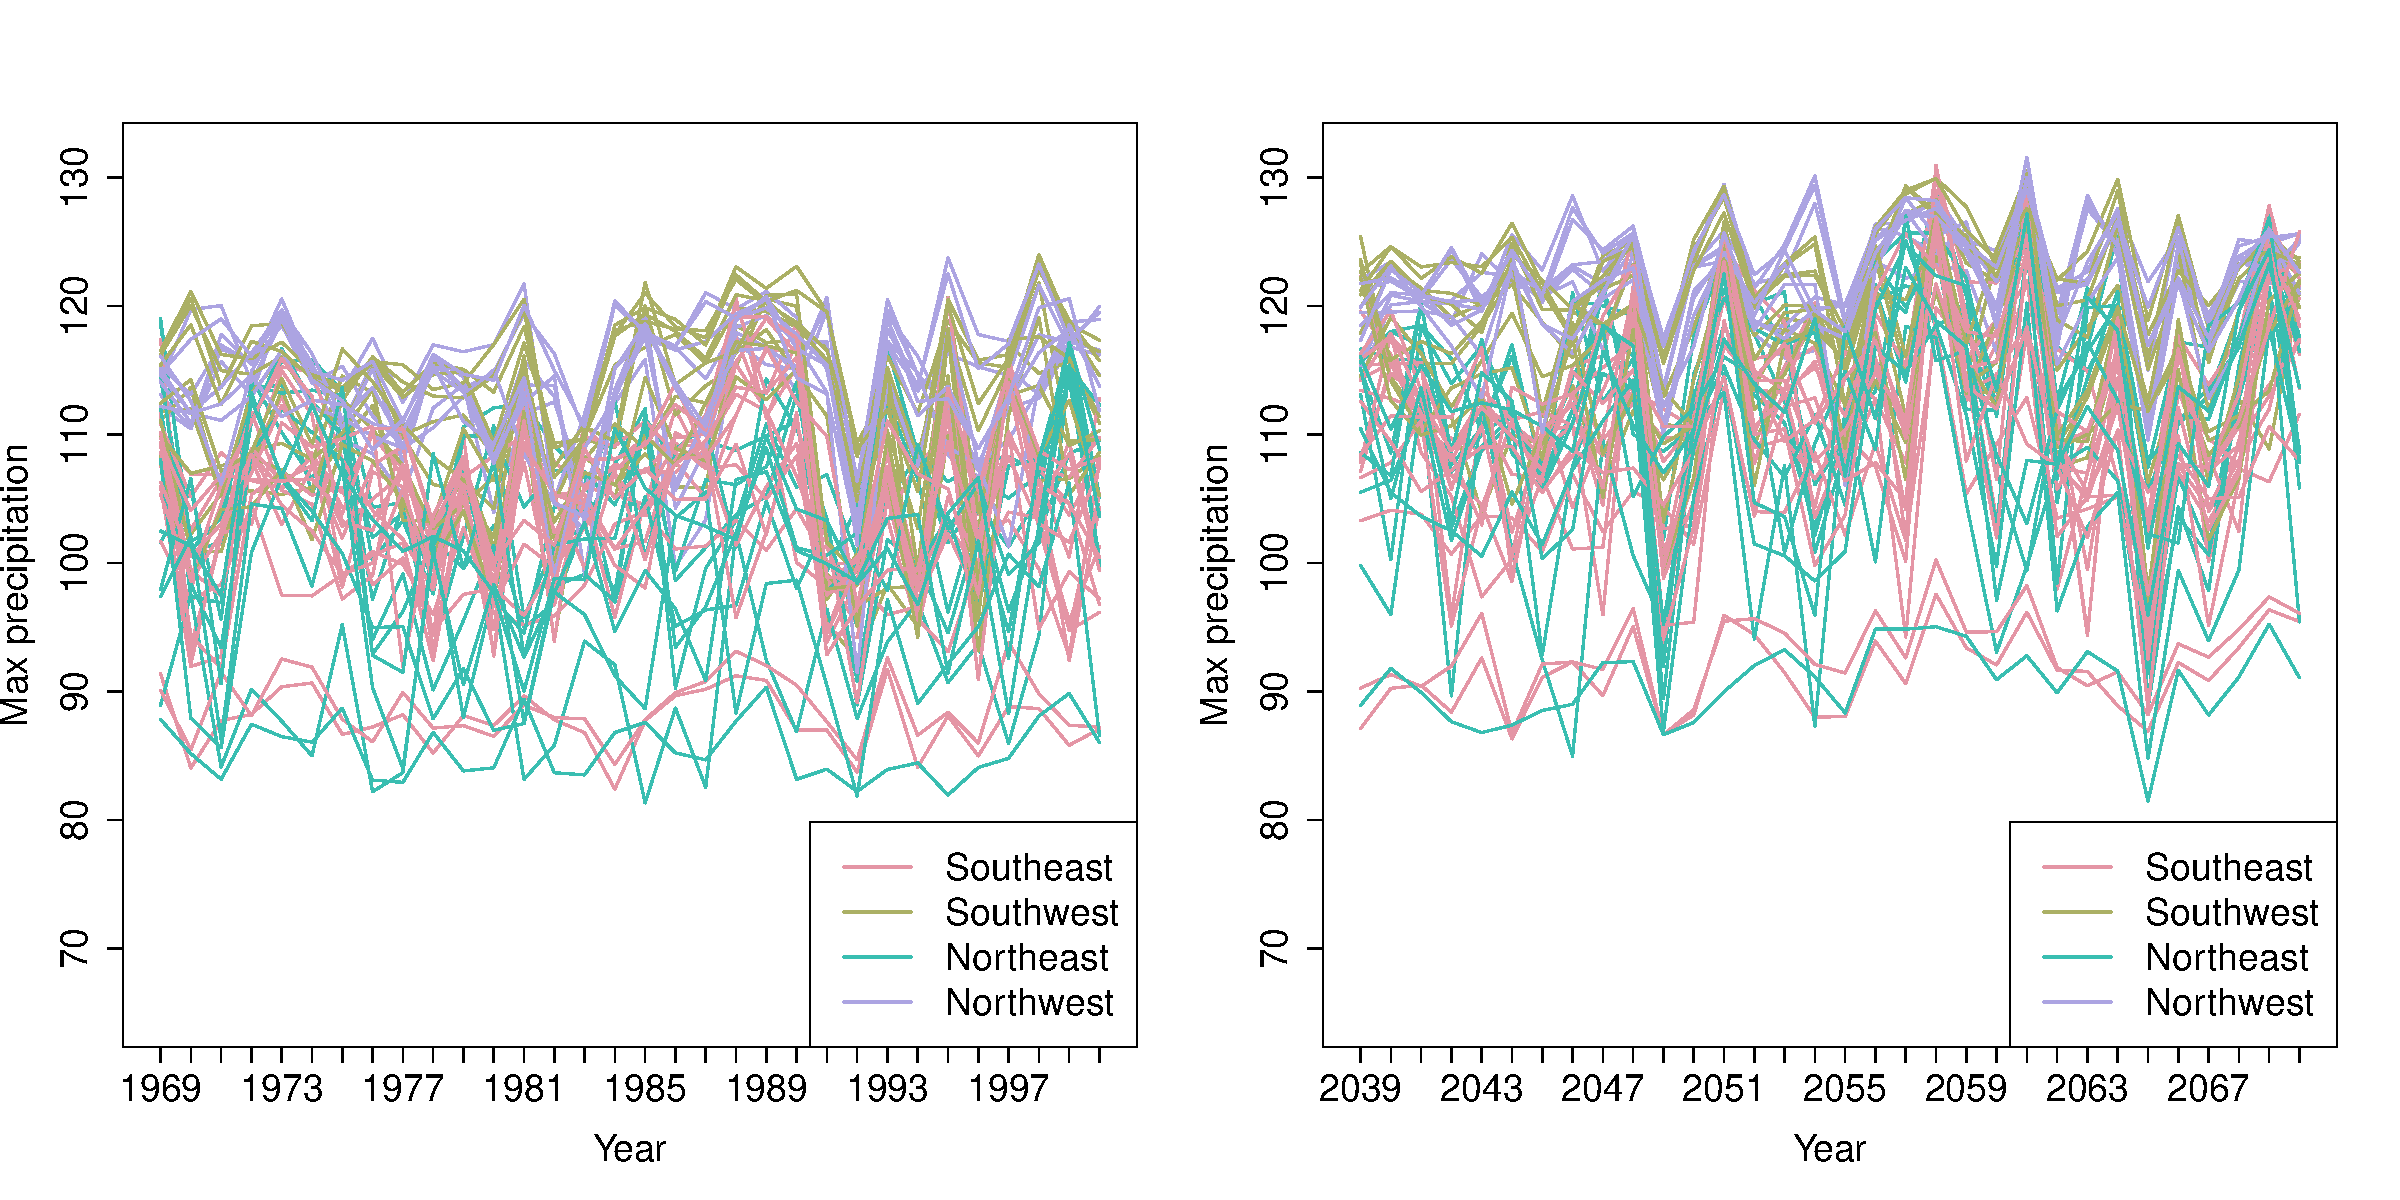
\includegraphics[width=\linewidth]{plots/precip-ts}
  \caption{Time series of yearly max precipitation for current (1969 -- 2000) (left). Time series of yearly max precipitation for future (2039 -- 2070) (right).}
  \label{ebfig:tsprecip}
\end{figure}

For this dataset, to estimate the EBFs, we use the combined current and future data.
The first six EBFs for the combined data along with the cumulative sum of the contributions for $v_1, \ldots, v_{25}$ are given in \fref{ebfig:precip-ebfpanel}.
\begin{figure}[htbp]  % markdown/precipitation/cv-setup.R
  \centering
  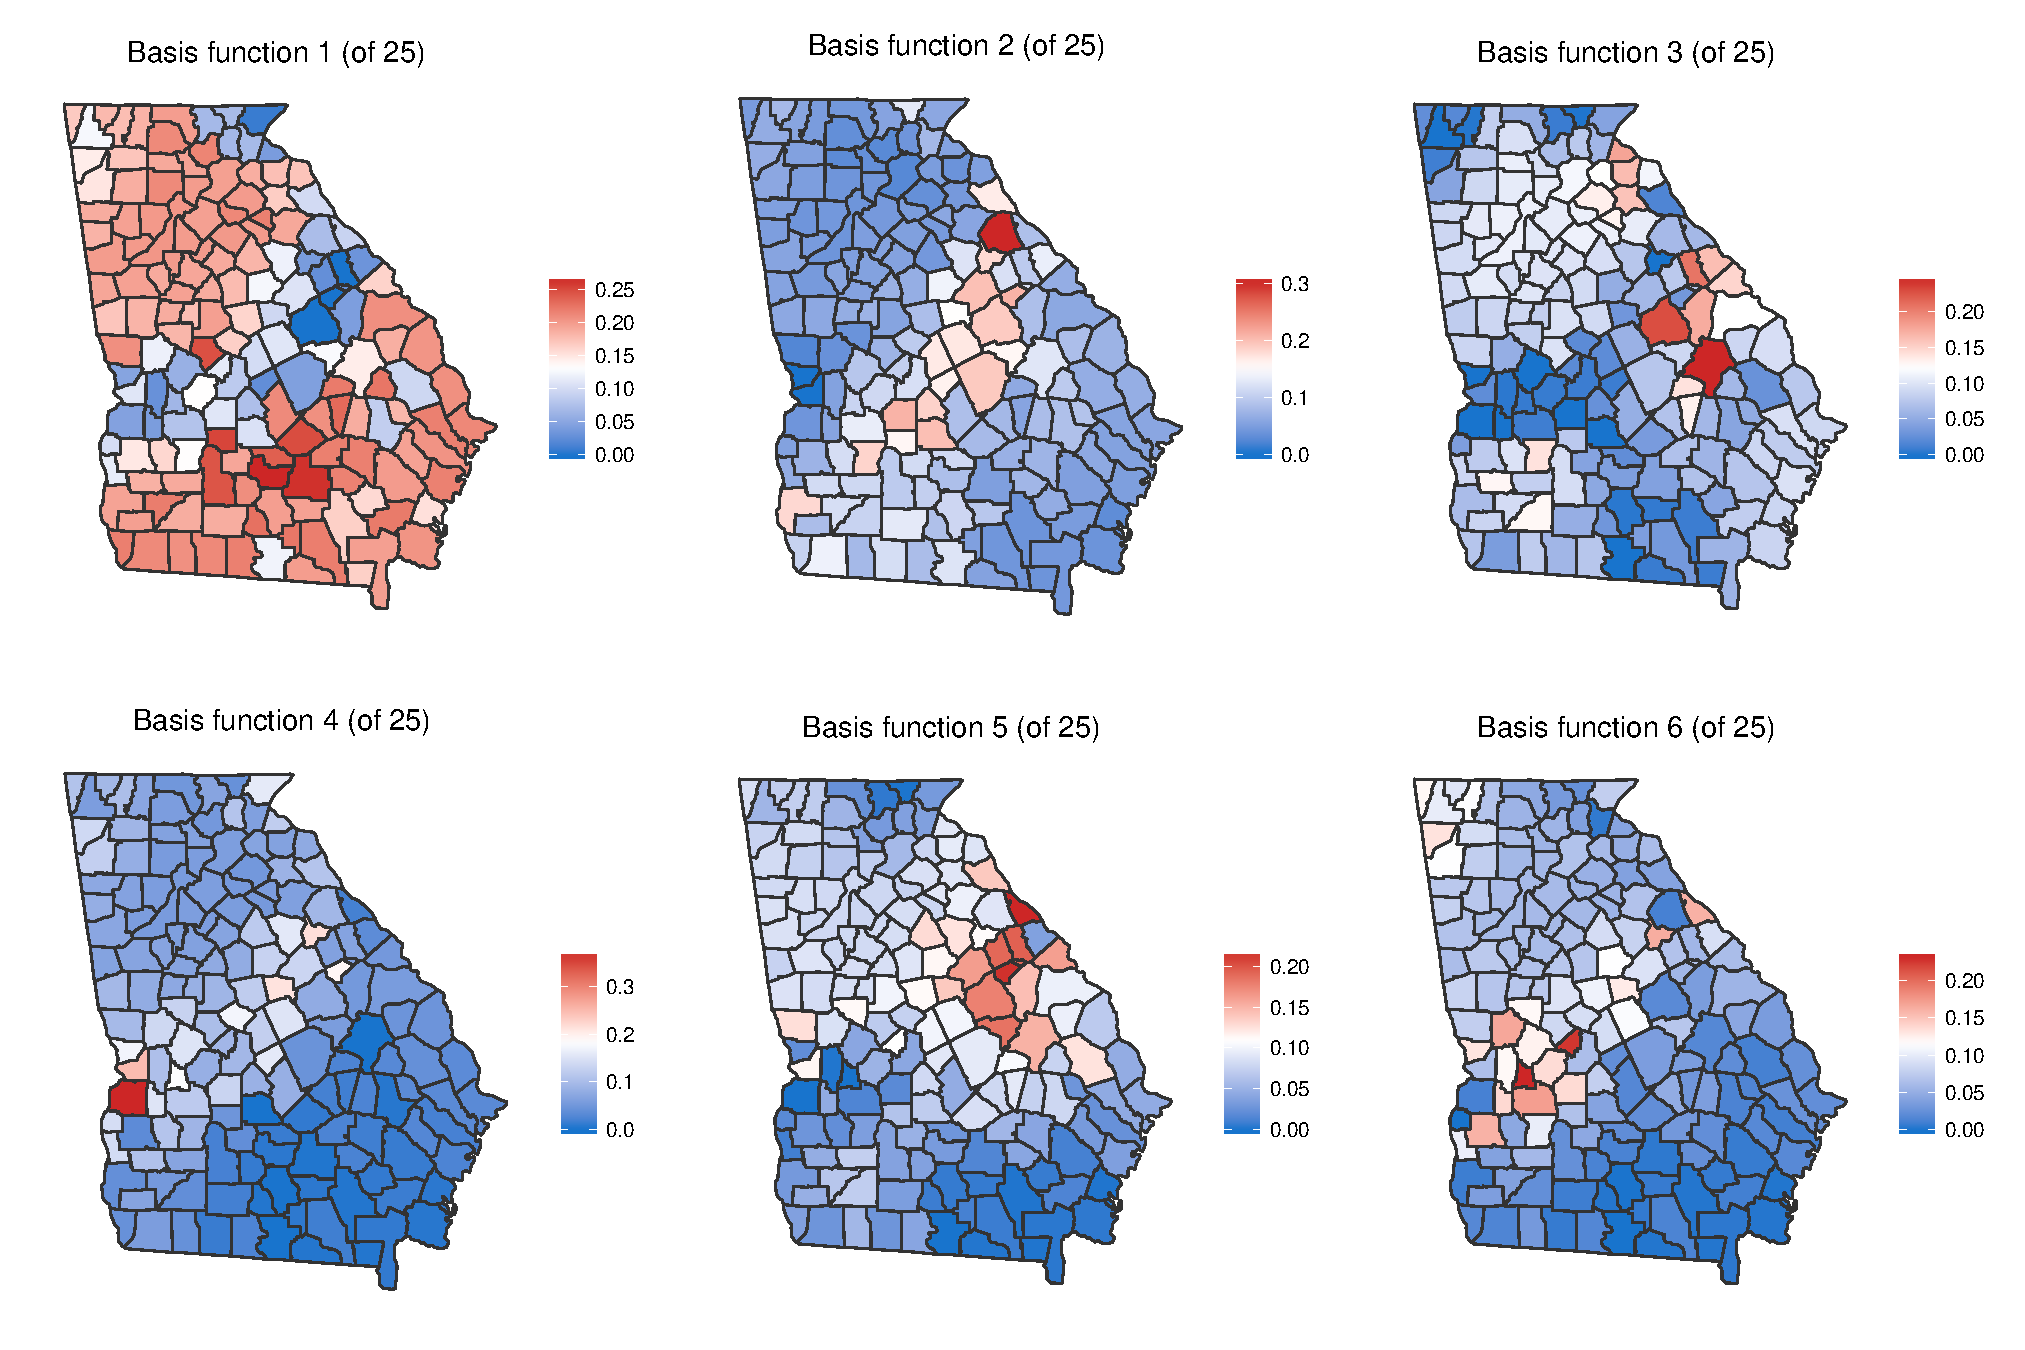
\includegraphics[width=\linewidth]{plots/precip-ebf-panel.pdf}\\
  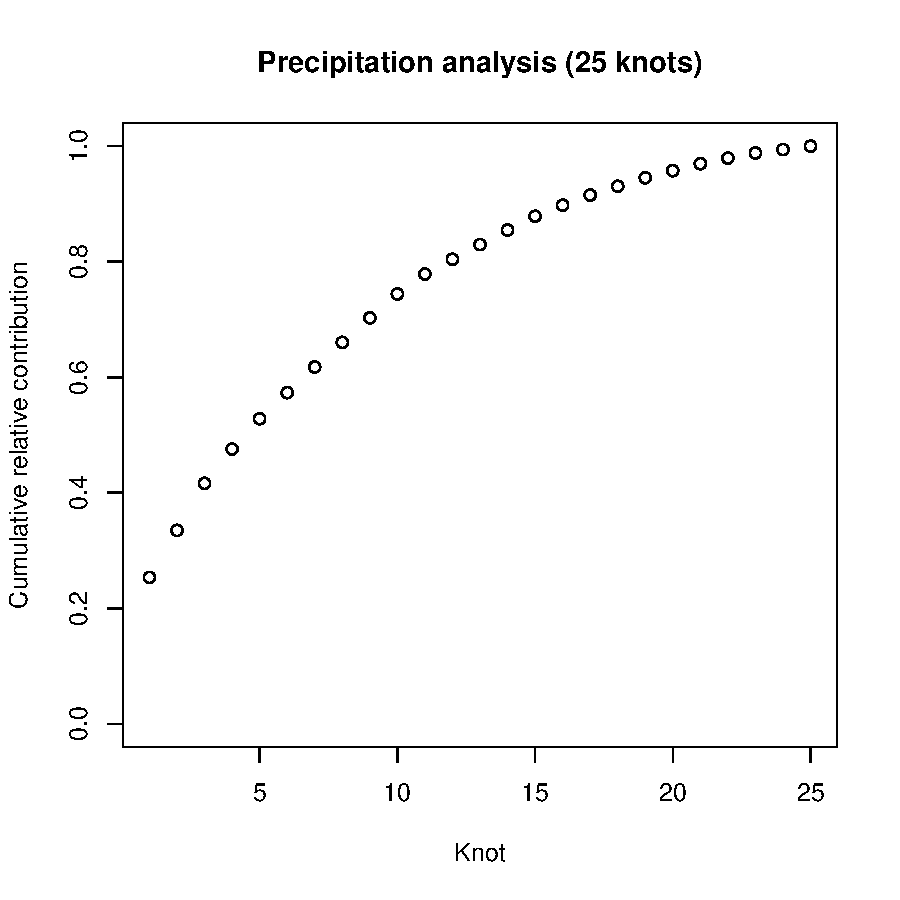
\includegraphics[width=0.35\linewidth]{plots/precipv-25.pdf}
  \caption{First six EBFs for the combined precipitation data and the cumulative sum of contributions $v_1, \ldots, v_{25}$.}
  \label{ebfig:precip-ebfpanel}
\end{figure}
As a comparison, we provide the first six principal components of the fire data along with the cumulative sum of the first 25 eigenvalues in \aref{eba:pca}.
For the precipitation data, we run the MCMC for 25,000 iterations using a burnin period of 15,000 iterations.
We consider models fit with both EBF and GSK, and fit the model using $L = 5, 10, \ldots, 40$.
Timing for each setting of $L$ is given in \tref{ebtbl:precip-scores} for 1,000.
These timings come from a single core of an Intel Core i7-5820K Haswell-E processor, using the OpenBLAS optimized BLAS library (\url{http://www.openblas.net}).

\subsection{Precipitation results} \label{ebs:results-precip}

We use 5-fold cross-validation to assess the predictive performance of a model.
For each method, we randomly select 80\% of the observations across counties and years to be used as a training set to fit the model.
The remaining 20\% of sites and years are withheld for testing model predictions.
To assess the predictions for the test set, we use quantile scores and Brier scores \citep{Gneiting2007}.
The quantile score (QS) for quantile level $q^*$ is given by \mbox{$2 \{I[Y(\bs) > \hat{q}(\bs)] - q^*]\}\{\hat{q}(\bs) - Y(\bs)\}$} where $\hat{q}(\bs)$ is the estimated $q^*$th quantile at site $\bs$, and $I[\cdot]$ is an indicator function.
The Brier score (BS) for predicting an exceedance of a level $c$ at site $\bs$ is given by \mbox{$\{I[Y(\bs) > c] - \hat{P}[Y(\bs) > c]\}^2$}.
For both of these methods, a lower score indicates a better fit.
We also present the Continuous Rank Probability Score (CRPS) \citep[see equation (21)]{Gneiting2007} and mean absolute deviation (MAD).
The Brier and quantile scores for the current and future precipitation data analysis are given in \tref{ebtbl:precip-scores}.
For these data, we observe more variation in the scores across the number of basis functions and generally an advantage in using EBF over GSK.
%This is in contrast to the fire analysis, and is likely due to the fact that the spatial dependence is estimated to be much stronger than for the fire analysis.
When using the EBFs, the estimate of residual dependence for the precipitation data is $\hat{\alpha} = 0.280$ ($\alpha = 1$ is residual independence).

Based on the cross-validation results, we run a full analysis using all of the data with $L = 25$ and EBF.
\fref{ebfig:precip-ebf-postpanel} gives posterior summaries for three quantities of interest.
Because we have two separate time periods, current and future, we look at the differences between the estimates for $\hat{\mu}$, $\log(\hat{\sigma})$, and $Q90$ between $t_1 = 2000$ and $t_2 = 2070$.

We construct the posterior distribution of the the estimated 90th quantile $Q90_{i, t}$ using the GEV parameters as follows.
Let $Q90_{i, t}^{(j)}$ be the estimated 90th quantile at site $i$ for time $t$ at iteration $j$.
We first compute
\begin{align}
  \mu_{i, t}^{(j)} &= \beta_{1, \text{int}, i}^{(j)} + \beta_{1, \text{time}, i}^{(j)} t \\
  \log\left(\sigma_{i, t}^{(j)}\right) &= \beta_{2, \text{int}, i}^{(j)} + \beta_{2, \text{time}, i}^{(j)} t. \nonumber
\end{align}
Let $Q90_{i, t}^{(j)} = \mu_{i, t}^{(j)} + \sigma_{i, t}^{(j)} F^{-1}\left(0.90, \xi^{(j)}\right)$ where $F^{-1}(q, \xi)$ is the inverse distribution function of the GEV$(1, 1, \xi)$ distribution evaluated at the $q$th quantile.
We summarize $hat{\mu}_{i, t}$, $\log(\hat{\sigma})_{i, t}$, and $Q90_{i, t}$ with the respective posterior means.
To obtain the posterior probability of seeing an increase over time, we take the posterior distributions of each parameter of interest at the two time points.
Consider two time points $t_1 < t_2$.
Let $\varphi_t^{(j)}$ be the parameter of interest at iteration $j$ and time $t$.
We then take the posterior mean of $I\left[\varphi_{t_2}^{(j)} > \varphi_{t_1}^{(j)}\right]$, for the posterior probability of seeing an increase in $\varphi$ from time $t_1$ to $t_2$.
We plot \mbox{$\Delta \mu = \hat{\mu}_{2070} - \hat{\mu}_{2000}$}, \mbox{$\Delta \log(\hat{\sigma}) = \log(\hat{\sigma})_{2070} - \log(\hat{\sigma})_{2000}$}, and \mbox{$\Delta Q90 = \hat{q}(0.90)_{2070} - \hat{q}(0.90)_{2000}$}, and the estimated probabilites that each are positive.

The results seem to suggest that the strength of extreme rain events will increases between 2000 and 2070 as well as greater variability in the northeast region of the U.S. as well as Ohio and parts of the south.
There very strong evidence to suggest that most of the eastern U.S. should expect to see an increase in the 10-year return level between 2000 and 2070.
Exceptions to this trend appear in southern parts of Alabama and Mississippi and regions on the border between South Carolina and Georgia which will likely experience a decrease in the 10-year return level.

\section{Discussion}\label{ebs:con}

In this paper we have proposed new empirical basis functions for a data-driven low-rank approximation to a max-stable process.
The basis functions provide researchers with an exploratory data analysis tool to explore maps of extremal dependence over space.
The functions can also be used as inputs to an MCMC algorithm for inference and predicitons over space.
The results from the data analysis provide evidence to suggest that in the presence of strong spatial dependence as with the precipitation data, the empirical basis functions show an improvement in quantile scores over using knots and standardized Gaussian kernel functions without an increase in the amount of time for computing.

We have used the EBF for exploratory analysis and Bayesian inference.
Another possibility is to use the methods to reduce the data under consideration from the actual responses to loadings $A_{kt}$.
That is, given the EBF, one could obtain estimates of the $A_{kt}$ using a separate maximum likelihood estimation for each time point.
Time series of the estimated $A_{kt}$ may be used as a fast and simple method to study large-scale spatiotemporal trends.

\begin{table}[htbp]
  \caption{Average Brier scores ($\times 100$), average quantile scores for $q(0.95)$ and $q(0.99)$, CRPS, MAD, and time (in minutes) for 1,000 iterations for current precipitation analysis.}
  \label{ebtbl:precip-scores}
  \footnotesize
  \centering
  \begin{tabular}{cc c cc c cc c c c c c c}
    \toprule
    & && \multicolumn{2}{c}{BS ($\times 100$)} && \multicolumn{2}{c}{QS} &&&&&& \\
    \cmidrule{4-5} \cmidrule{7-8}
    $L$ & Process & \phantom{a} & $q(0.95)$ & $q(0.99)$ & \phantom{a} & $q(0.95)$ & $q(0.99)$ & \phantom{a} & CRPS & \phantom{a} & MAD & \phantom{a} & Time\\
   \midrule																	
2	&	EBF	&&	4.189	&	1.194	&&	0.842	&	0.244	&&	2.297	&&	3.176	&&	4.85	\\
	&	GSK	&&	4.144	&	1.193	&&	0.885	&	0.250	&&	2.388	&&	3.312	&&	4.88	\\
\midrule																	
3	&	EBF	&&	3.973	&	1.105	&&	0.793	&	0.222	&&	2.108	&&	2.901	&&	4.96	\\
	&	GSK	&&	4.015	&	1.070	&&	0.804	&	0.225	&&	2.142	&&	2.952	&&	4.97	\\
\midrule																	
5	&	EBF	&&	3.623	&	1.022	&&	0.737	&	0.207	&&	1.947	&&	2.666	&&	5.18	\\
	&	GSK	&&	3.765	&	1.016	&&	0.756	&	0.210	&&	1.941	&&	2.658	&&	5.19	\\
\midrule																	
10	&	EBF	&&	3.691	&	1.192	&&	0.727	&	0.212	&&	1.818	&&	2.455	&&	5.69	\\
	&	GSK	&&	3.813	&	1.491	&&	0.803	&	0.256	&&	1.771	&&	2.366	&&	5.71	\\
\midrule																	
15	&	EBF	&&	3.815	&	1.529	&&	0.781	&	0.246	&&	1.791	&&	2.394	&&	6.27	\\
	&	GSK	&&	3.898	&	1.652	&&	0.832	&	0.272	&&	1.722	&&	2.267	&&	6.30	\\
\midrule																	
20	&	EBF	&&	3.858	&	1.651	&&	0.788	&	0.252	&&	1.740	&&	2.296	&&	6.86	\\
	&	GSK	&&	3.908	&	1.715	&&	0.848	&	0.281	&&	1.689	&&	2.204	&&	6.87	\\
\midrule																	
25	&	EBF	&&	4.080	&	1.776	&&	0.802	&	0.255	&&	1.754	&&	2.298	&&	7.43	\\
	&	GSK	&&	3.906	&	1.760	&&	0.852	&	0.284	&&	1.676	&&	2.177	&&	7.46	\\
\midrule																	
30	&	EBF	&&	4.029	&	1.827	&&	0.794	&	0.257	&&	1.716	&&	2.235	&&	8.00	\\
	&	GSK	&&	3.965	&	1.799	&&	0.859	&	0.288	&&	1.670	&&	2.160	&&	8.00	\\
\midrule																	
35	&	EBF	&&	4.107	&	1.850	&&	0.801	&	0.257	&&	1.730	&&	2.246	&&	8.56	\\
	&	GSK	&&	3.959	&	1.799	&&	0.860	&	0.290	&&	1.656	&&	2.139	&&	8.61	\\
\midrule																	
40	&	EBF	&&	4.063	&	1.889	&&	0.808	&	0.261	&&	1.748	&&	2.259	&&	9.14	\\
	&	GSK	&&	4.012	&	1.841	&&	0.868	&	0.293	&&	1.673	&&	2.160	&&	9.17	\\
\bottomrule																	
  \end{tabular}
\end{table}

\begin{table}[htbp]
	\caption{Average Brier scores ($\times 100$), average quantile scores for $q(0.95)$ and $q(0.99)$, CRPS, MAD, and time (in minutes) for 1,000 iterations for future precipitation analysis.}
	\label{ebtbl:precip-scores}
	\footnotesize
	\centering
	\begin{tabular}{cc c cc c cc c c c c c c}
		\toprule
		& && \multicolumn{2}{c}{BS ($\times 100$)} && \multicolumn{2}{c}{QS} &&&&&& \\
		\cmidrule{4-5} \cmidrule{7-8}
		$L$ & Process & \phantom{a} & $q(0.95)$ & $q(0.99)$ & \phantom{a} & $q(0.95)$ & $q(0.99)$ & \phantom{a} & CRPS & \phantom{a} & MAD & \phantom{a} & Time\\
		\midrule																	
2	&	EBF	&&	3.796	&	1.148	&&	0.840	&	0.237	&&	2.156	&&	2.947	&&	4.82	\\
	&	GSK	&&	3.470	&	1.142	&&	0.850	&	0.237	&&	2.145	&&	2.925	&&	4.82	\\
\midrule																	
3	&	EBF	&&	3.477	&	1.112	&&	0.785	&	0.220	&&	2.008	&&	2.747	&&	4.96	\\
	&	GSK	&&	3.075	&	1.039	&&	0.781	&	0.225	&&	1.963	&&	2.663	&&	4.96	\\
\midrule																	
5	&	EBF	&&	3.350	&	1.035	&&	0.724	&	0.204	&&	1.852	&&	2.526	&&	5.16	\\
	&	GSK	&&	3.219	&	1.046	&&	0.736	&	0.209	&&	1.846	&&	2.500	&&	5.15	\\
\midrule																	
10	&	EBF	&&	3.136	&	1.088	&&	0.692	&	0.203	&&	1.684	&&	2.257	&&	5.69	\\
	&	GSK	&&	3.020	&	1.118	&&	0.710	&	0.208	&&	1.668	&&	2.221	&&	5.72	\\
\midrule																	
15	&	EBF	&&	3.219	&	1.141	&&	0.697	&	0.205	&&	1.659	&&	2.207	&&	6.28	\\
	&	GSK	&&	3.078	&	1.222	&&	0.739	&	0.226	&&	1.641	&&	2.162	&&	6.32	\\
\midrule																	
20	&	EBF	&&	3.159	&	1.280	&&	0.703	&	0.211	&&	1.619	&&	2.133	&&	6.87	\\
	&	GSK	&&	3.175	&	1.369	&&	0.775	&	0.242	&&	1.634	&&	2.135	&&	6.91	\\
\midrule																	
25	&	EBF	&&	3.273	&	1.336	&&	0.723	&	0.221	&&	1.649	&&	2.159	&&	7.45	\\
	&	GSK	&&	3.198	&	1.467	&&	0.802	&	0.257	&&	1.625	&&	2.103	&&	7.47	\\
\midrule																	
30	&	EBF	&&	3.399	&	1.555	&&	0.771	&	0.243	&&	1.645	&&	2.125	&&	8.03	\\
	&	GSK	&&	3.320	&	1.609	&&	0.849	&	0.278	&&	1.648	&&	2.113	&&	8.04	\\
\midrule																	
35	&	EBF	&&	3.433	&	1.592	&&	0.755	&	0.239	&&	1.647	&&	2.121	&&	8.62	\\
	&	GSK	&&	3.378	&	1.668	&&	0.866	&	0.285	&&	1.644	&&	2.097	&&	8.60	\\
\midrule																	
40	&	EBF	&&	3.529	&	1.679	&&	0.791	&	0.252	&&	1.681	&&	2.145	&&	9.16	\\
	&	GSK	&&	3.418	&	1.690	&&	0.878	&	0.290	&&	1.656	&&	2.111	&&	9.19	\\
\bottomrule																	
	\end{tabular}
\end{table}

% \begin{figure}[htbp]  % markdown/precipitation/combine-tables.R
%   \centering
%   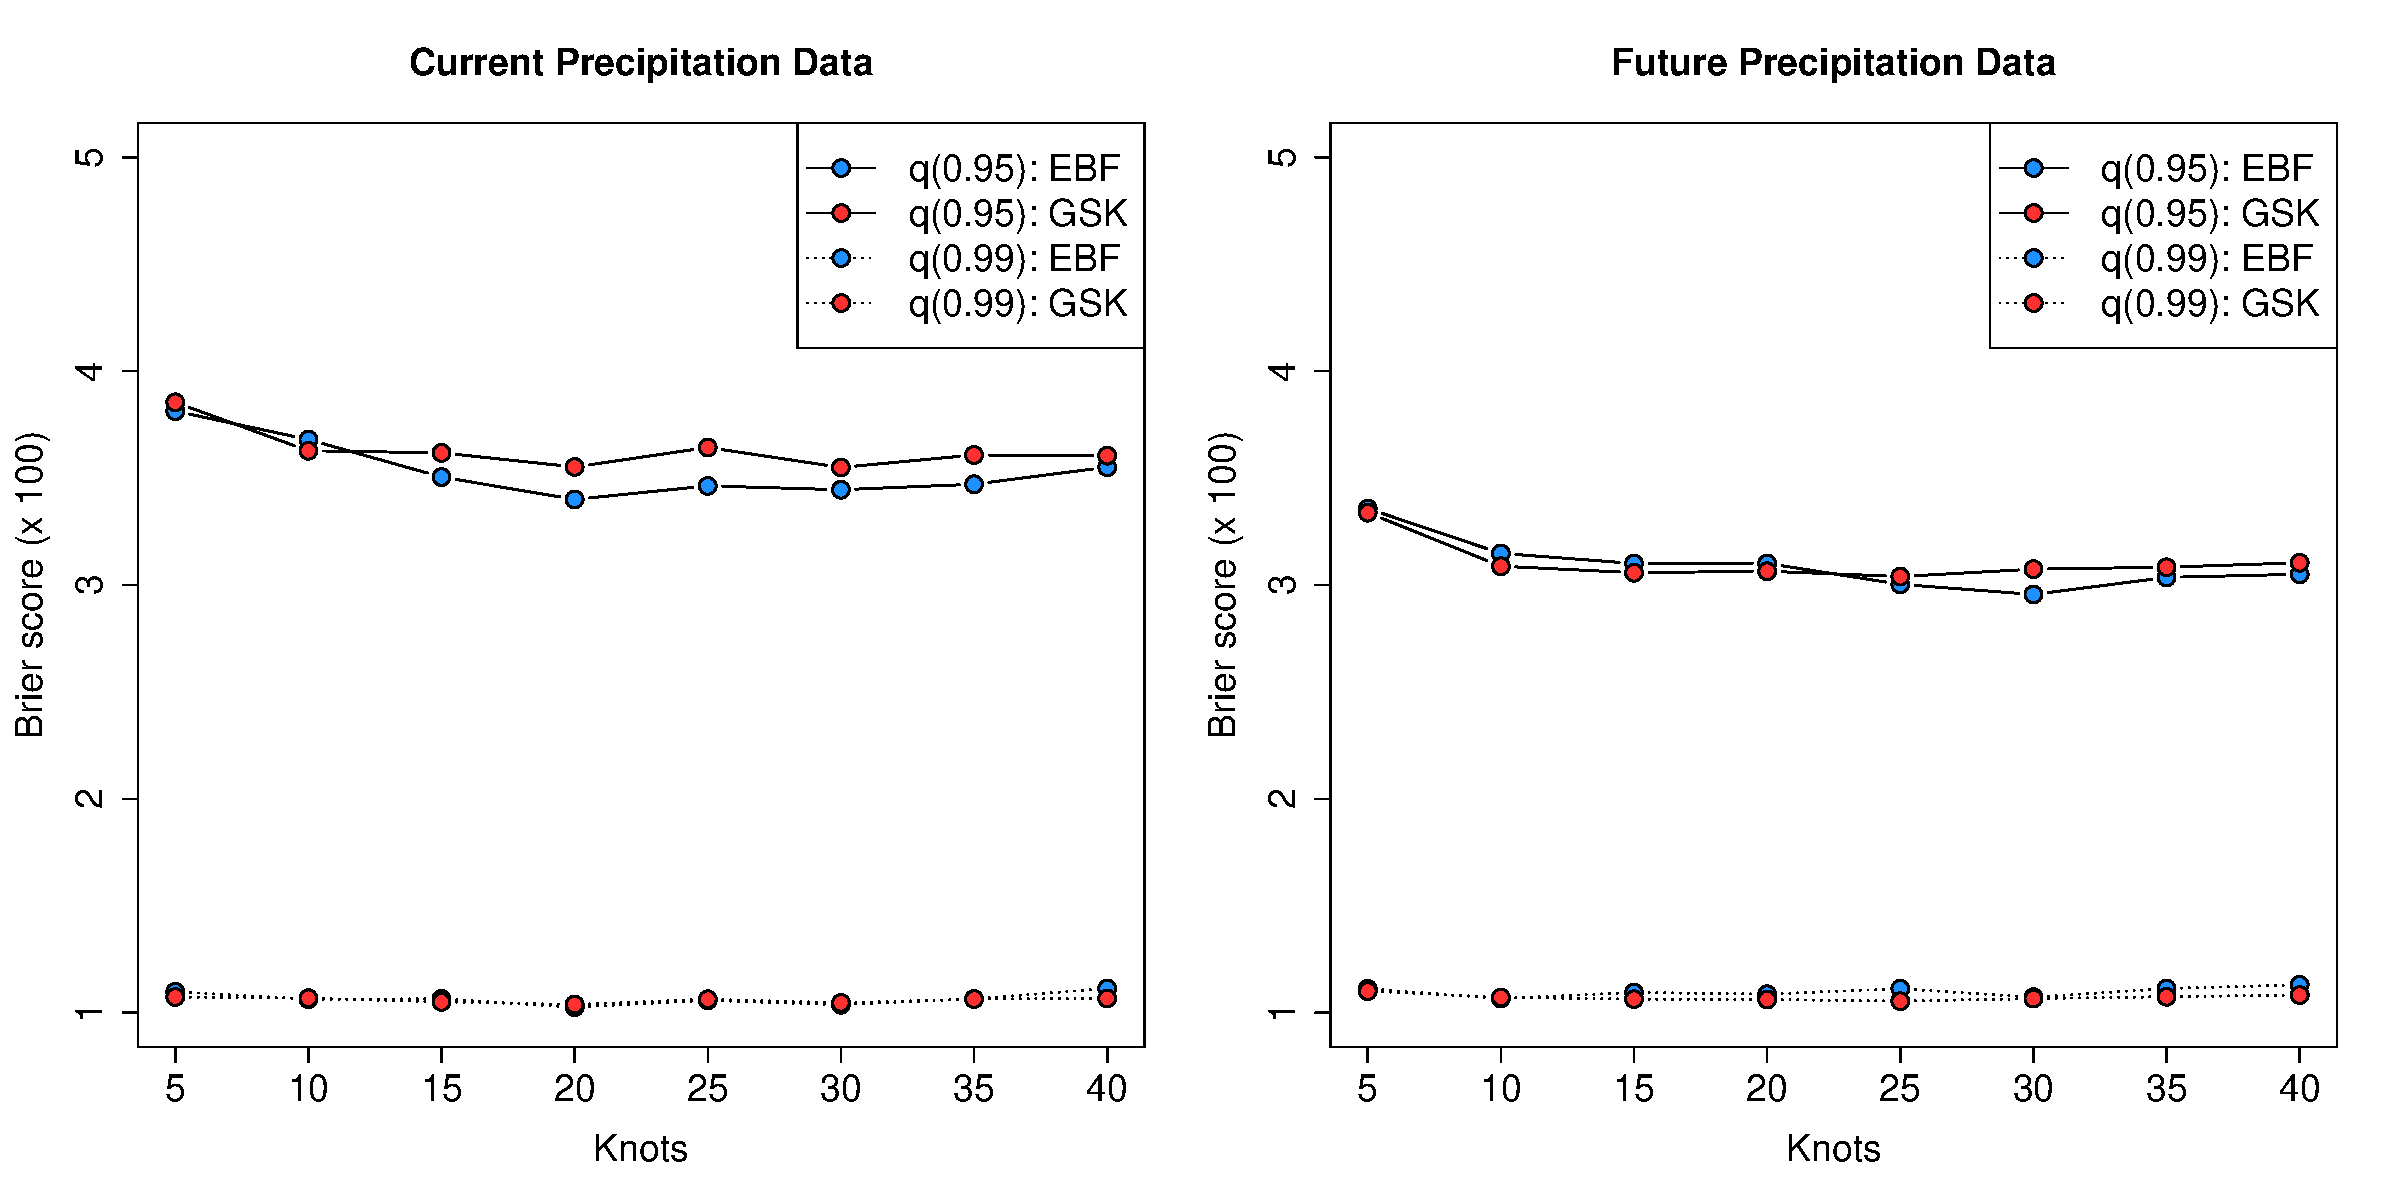
\includegraphics[width=\linewidth]{plots/precip-bs.pdf}
%   \caption{Brier scores for $q(0.95)$ and $q(0.99)$ to compare EBF and GSK analysis of precipitation data for current (left) and future (right).}
%   \label{ebfig:precip-bs}
% \end{figure}

% \begin{figure}[htbp]  % markdown/precipitation/combine-tables.R
%   \centering
%   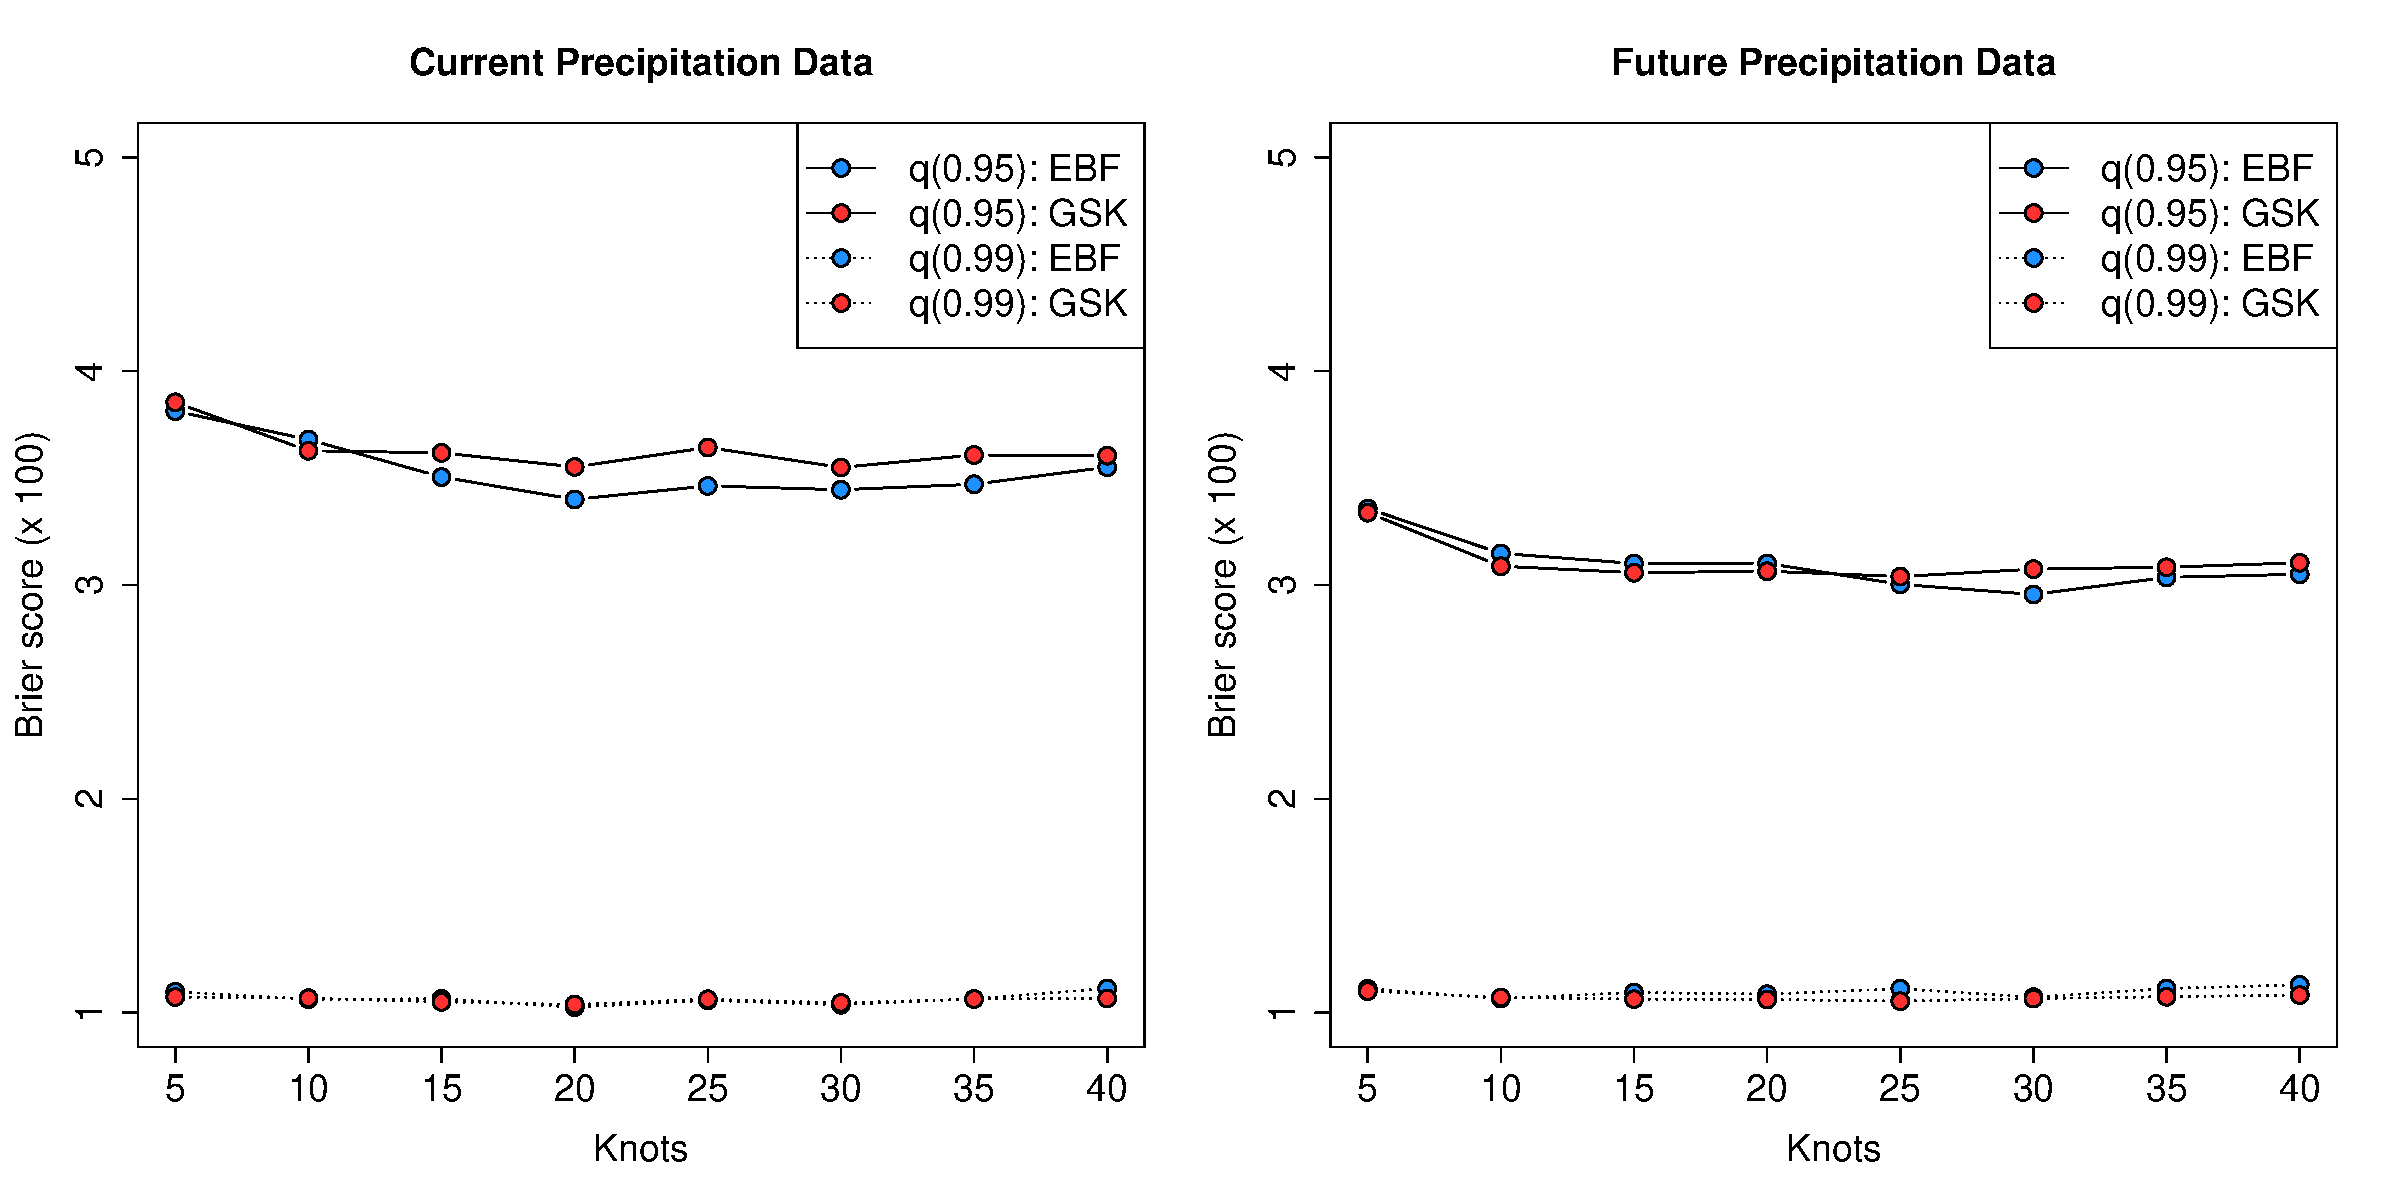
\includegraphics[width=\linewidth]{plots/precip-bs.pdf}
%   \caption{Quantile scores for $q(0.95)$ and $q(0.99)$ to compare EBF and GSK analysis of precipitation data for current (left) and future (right).}
%   \label{ebfig:precip-qs}
% \end{figure}

\begin{figure}[htbp]  % markdown/precipitation/posterior_map.R
  \centering
  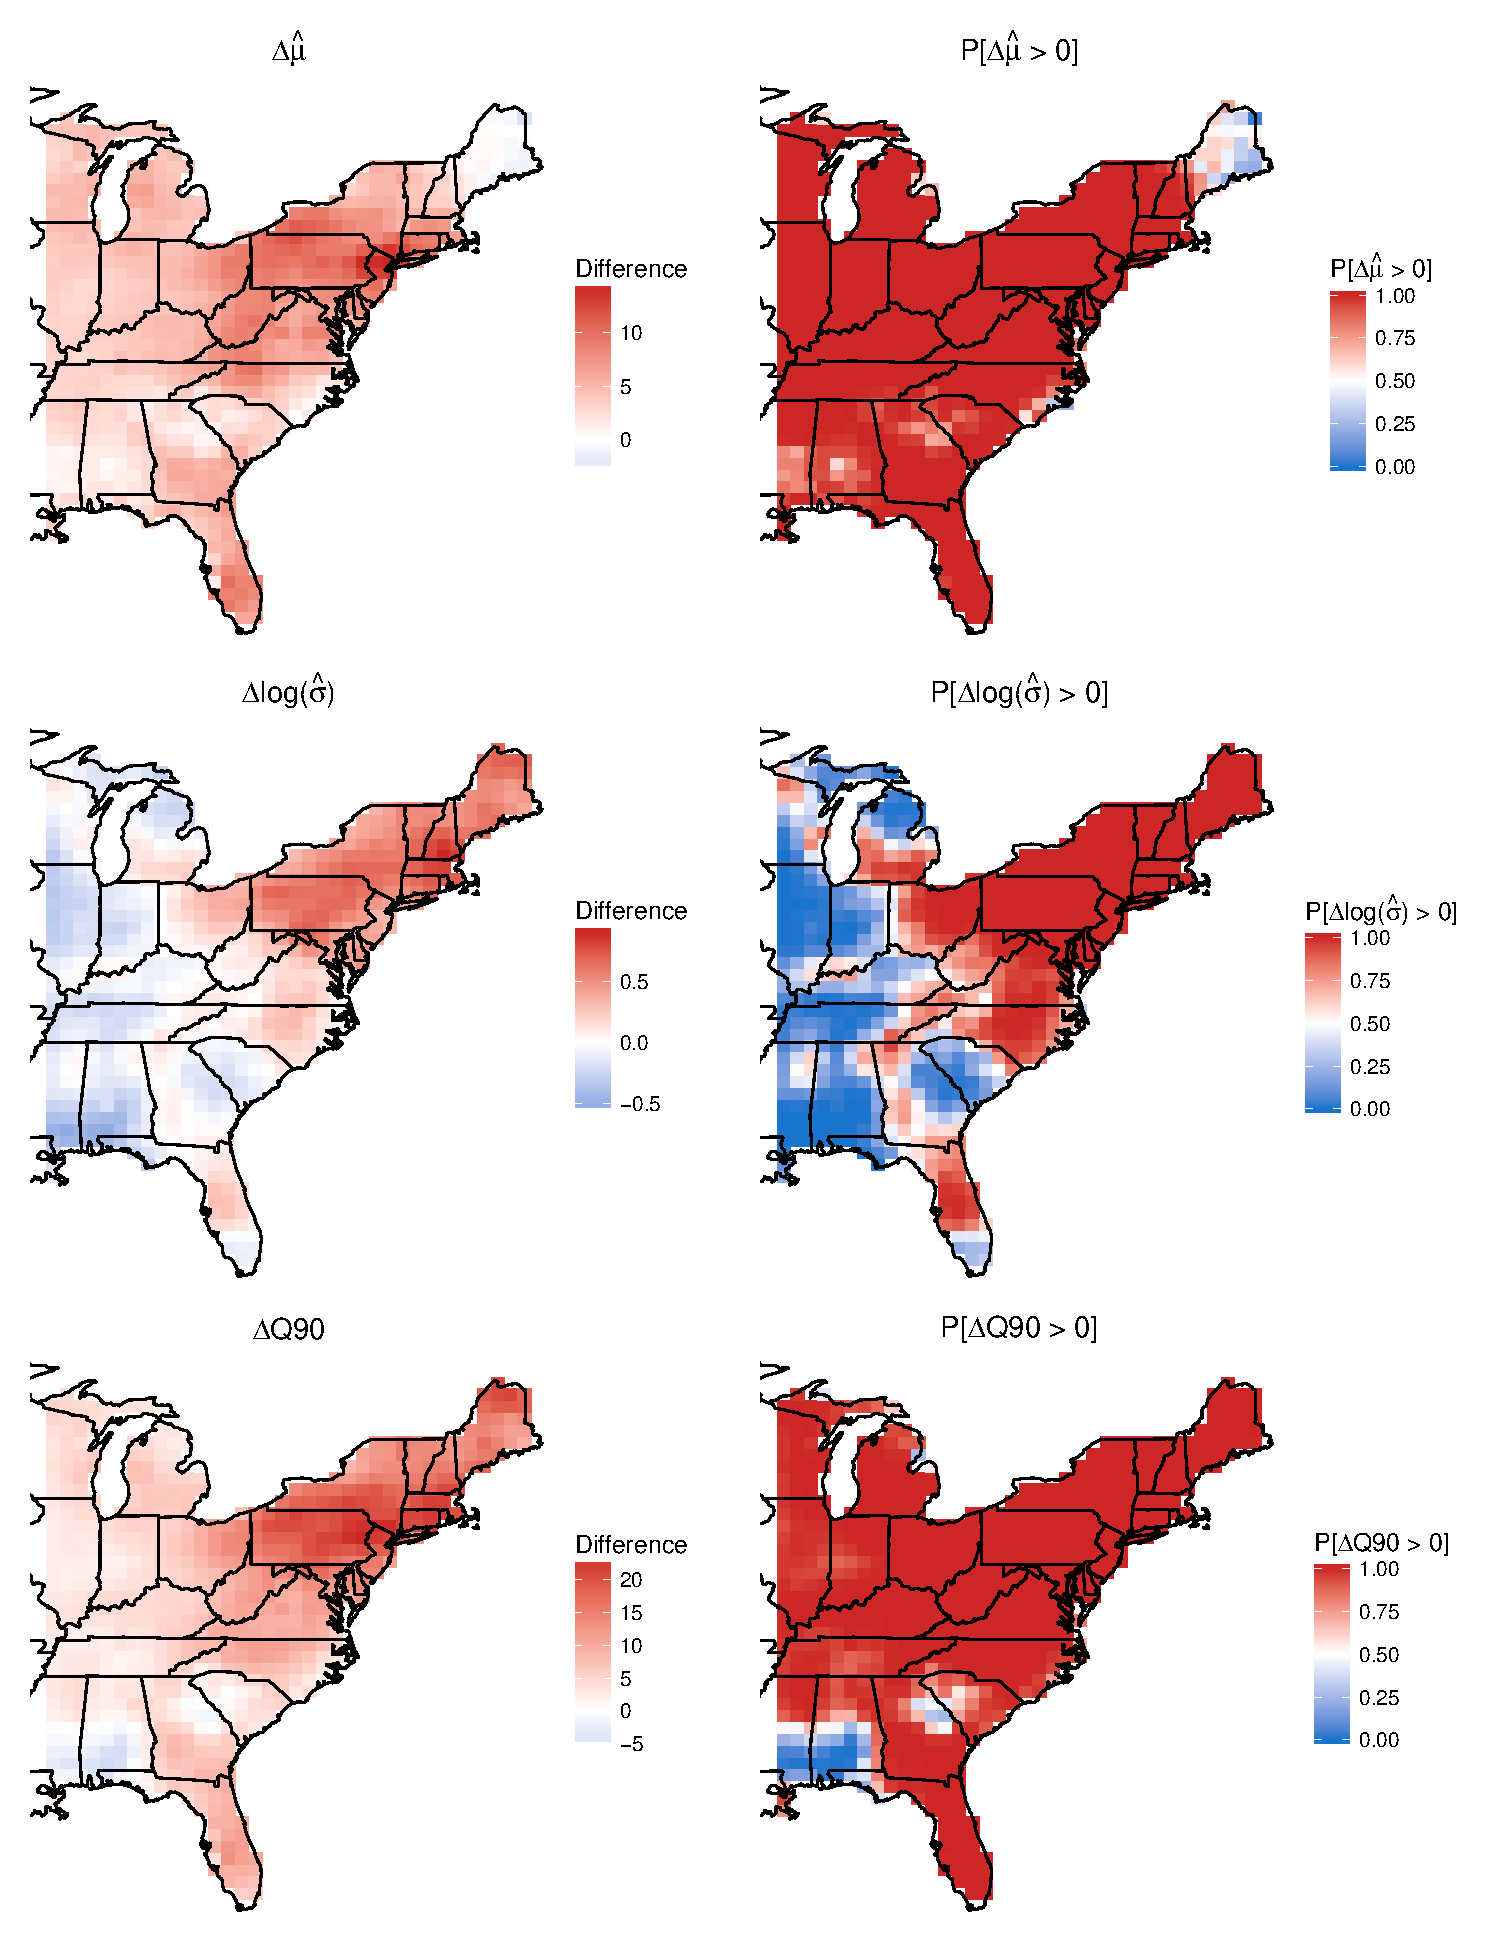
\includegraphics[height=0.9\textheight]{plots/precip-ebf-postpanel.pdf}
  \caption{Posterior mean of $\Delta \mu$ (top left), posterior mean of $\Delta \log(\sigma)$ (middle left), estimate of $\Delta Q90$ (bottom left), P$[\Delta \mu > 0]$ (top right), P$[\Delta \log(\sigma) > 0]$ (middle right), and P$[\Delta Q90 > 0]$ between 2000 and 2070 for precipitation data using EBF.}
  \label{ebfig:precip-ebf-postpanel}
\end{figure}

% \begin{figure}[htbp]  % markdown/precipitation/posterior_map.R
%   \centering
%   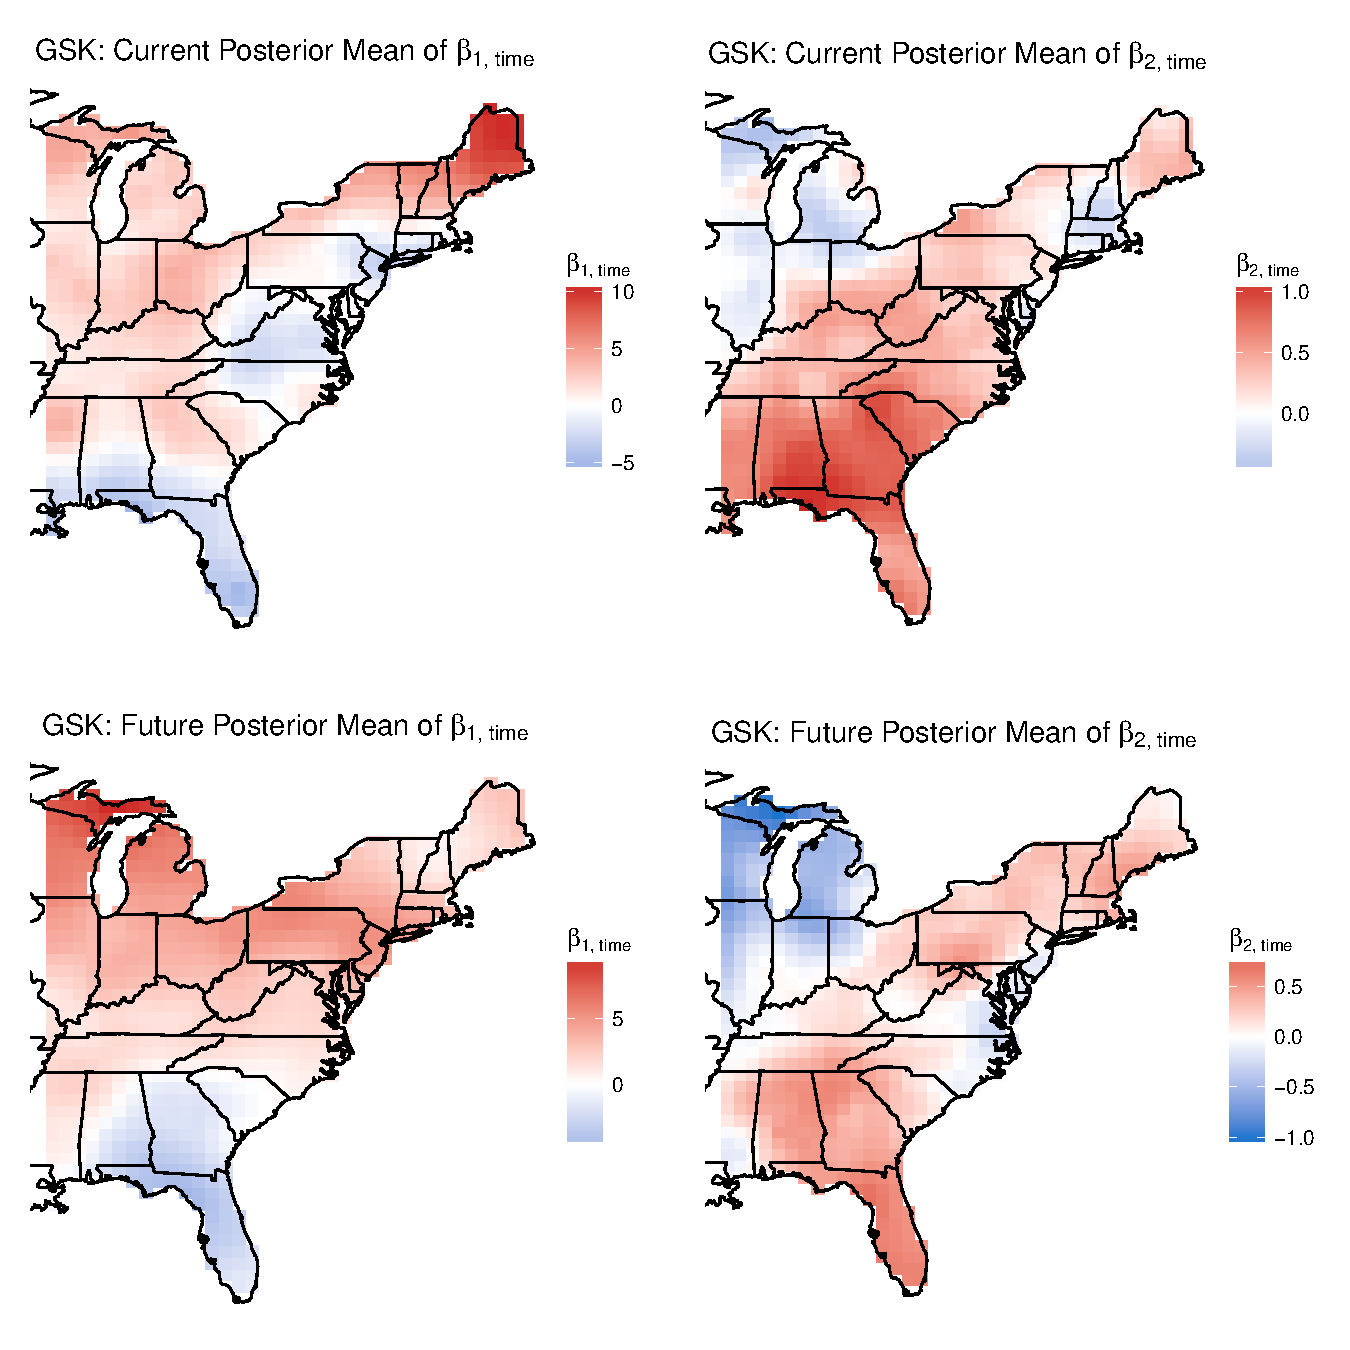
\includegraphics[width=\linewidth]{plots/precip-gsk-post-betatime.pdf}
%   \caption{Posterior mean of $\beta_{1, \text{time}}$ (left) and $\beta_{2, \text{time}}$ (right) for current (top) and future (bottom) precipitation data using GSK.}
%   \label{ebfig:fire-gskpostbeta1}
% \end{figure}

% \begin{figure}[htbp]  % markdown/precipitation/posterior_map.R
%   \centering
%   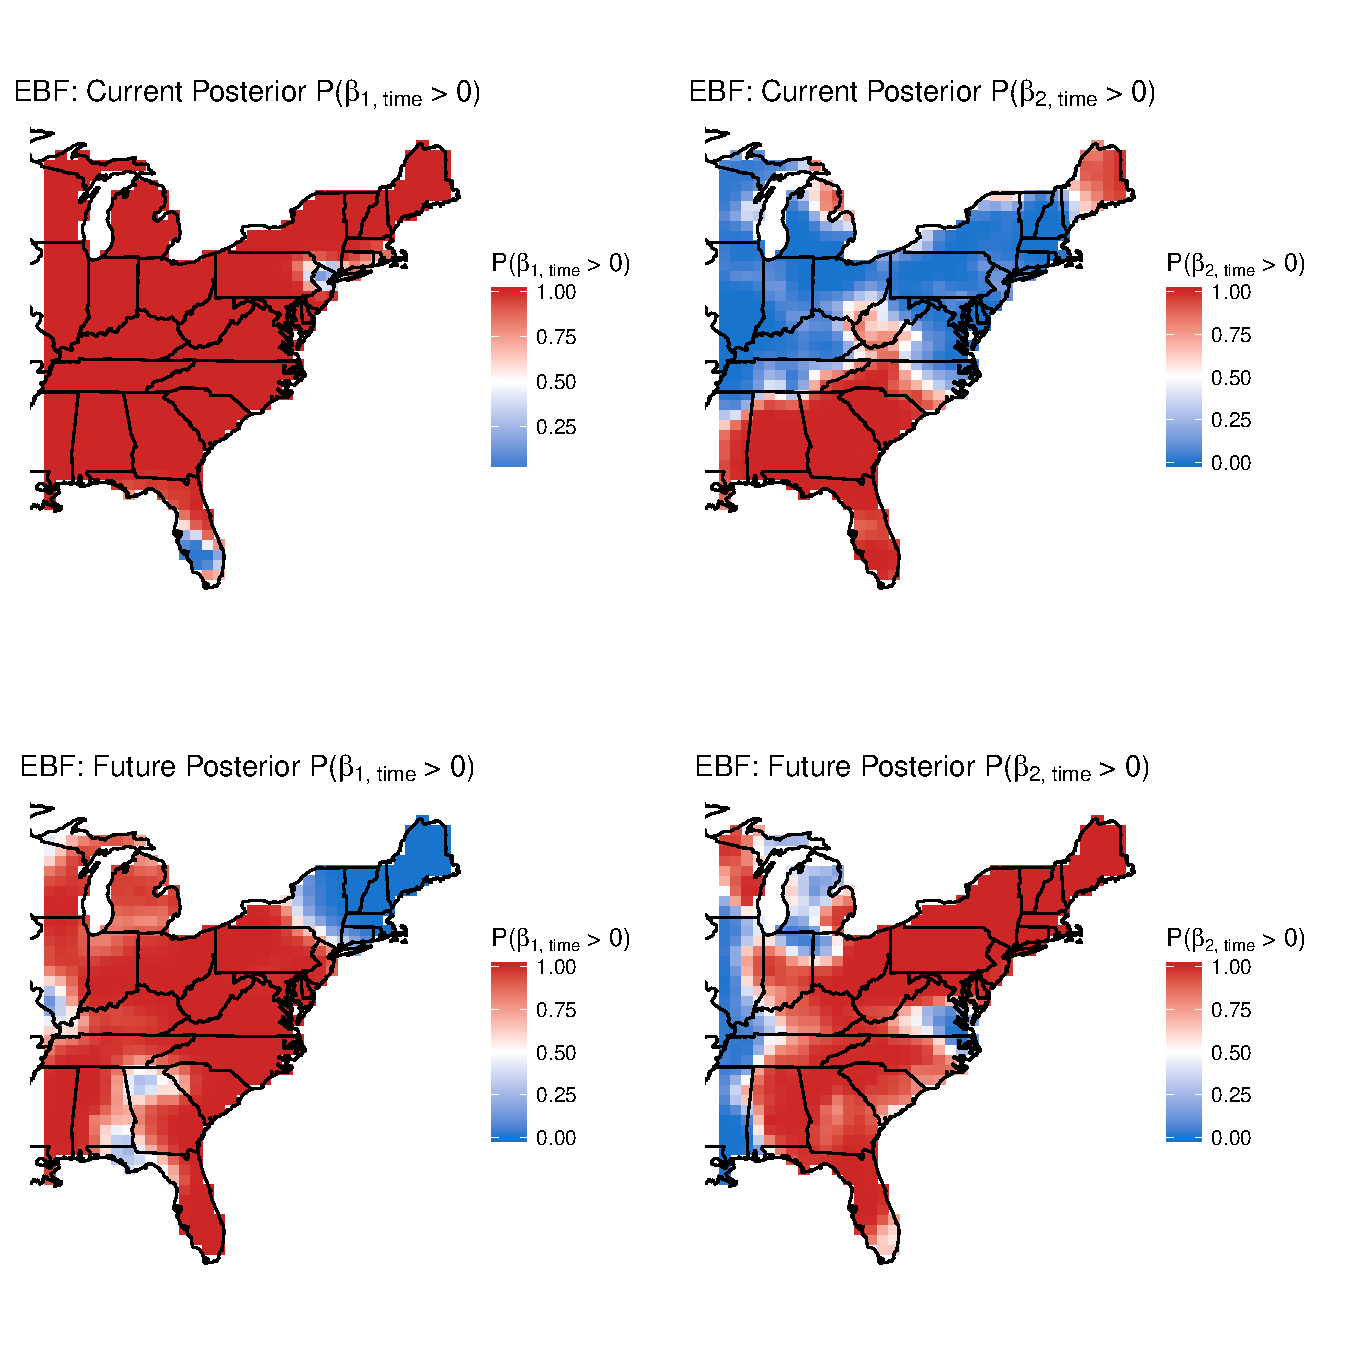
\includegraphics[width=\linewidth]{plots/precip-ebf-post-betatimepos.pdf}
%   \caption{Posterior P$(\beta_{1, \text{time}} > 0)$ (left) and P$(\beta_{2, \text{time}} > 0)$ (right) for current (top) and future (bottom) precipitation data using EBF.}
%   \label{ebfig:fire-ebfpostbeta1pos}
% \end{figure}

% \begin{figure}[htbp]  % markdown/precipitation/posterior_map.R
%   \centering
%   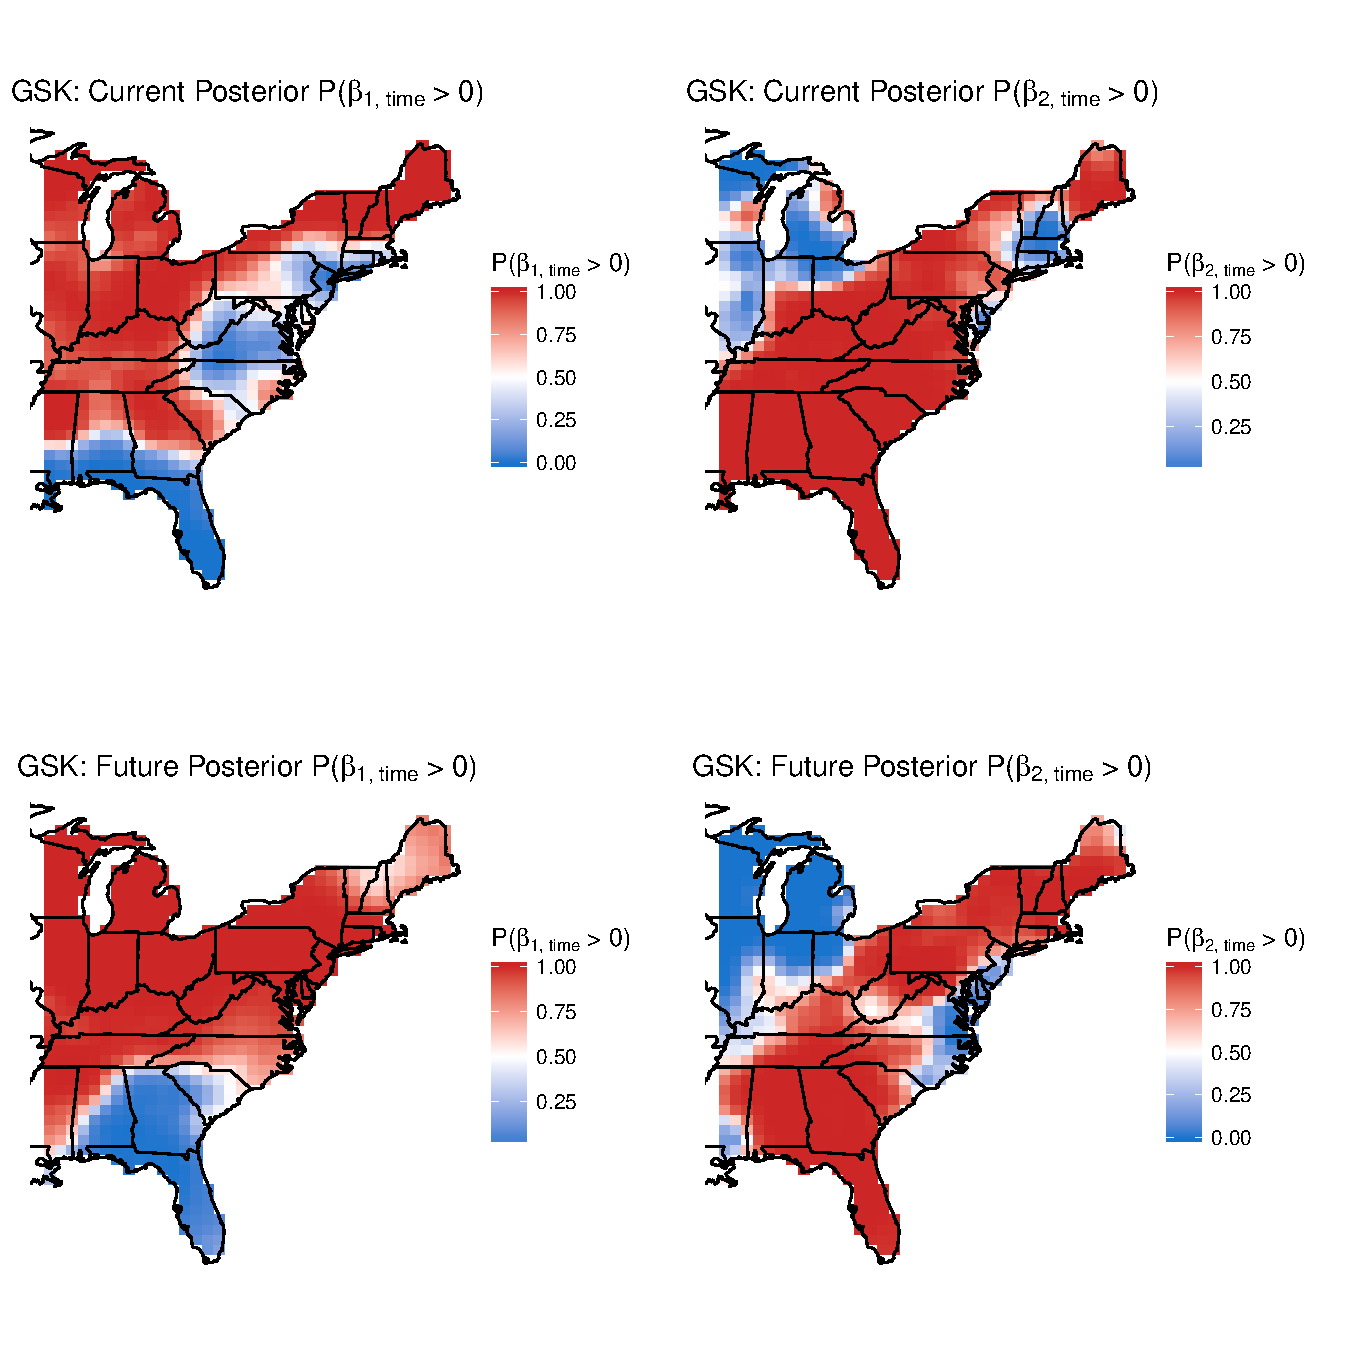
\includegraphics[width=\linewidth]{plots/precip-gsk-post-betatimepos.pdf}
%   \caption{Posterior P$(\beta_{1, \text{time}} > 0)$ (left) and P$(\beta_{2, \text{time}} > 0)$ (right) for current (top) and future (bottom) precipitation data using GSK.}
%   \label{ebfig:fire-gskpostbeta1pos}
% \end{figure}


% \begin{figure}[htbp]  % markdown/precipitation/posterior_map.R
%   \centering
%   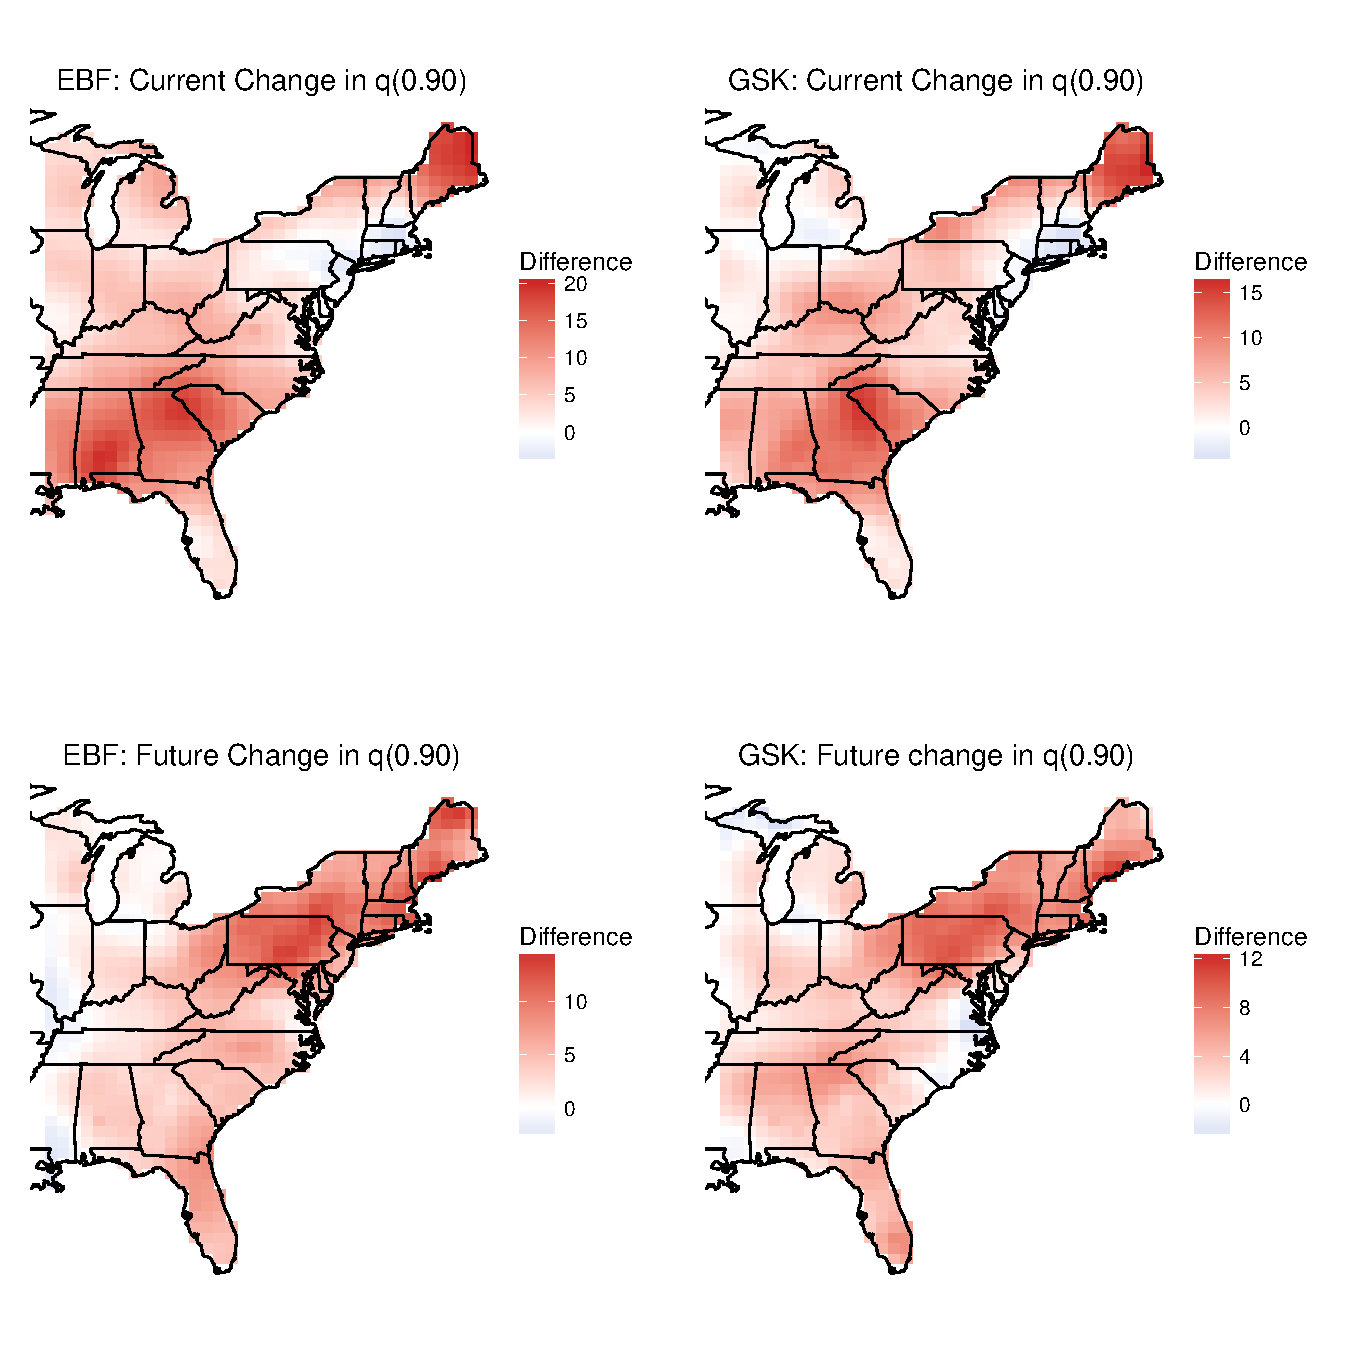
\includegraphics[width=\linewidth]{plots/precip-q90diff-compare.pdf}
%   \caption{Difference in $q(0.90)$ for precipitation data between 2000 and 1969 for current (top) and 2070 and 2039 for future (bottom) using EBF (left) and GSK (right).}
%   \label{ebfig:precip-q90diff}
% \end{figure}

% \begin{figure}  % markdown/precipitation/combine-tables.R
%   \centering
%   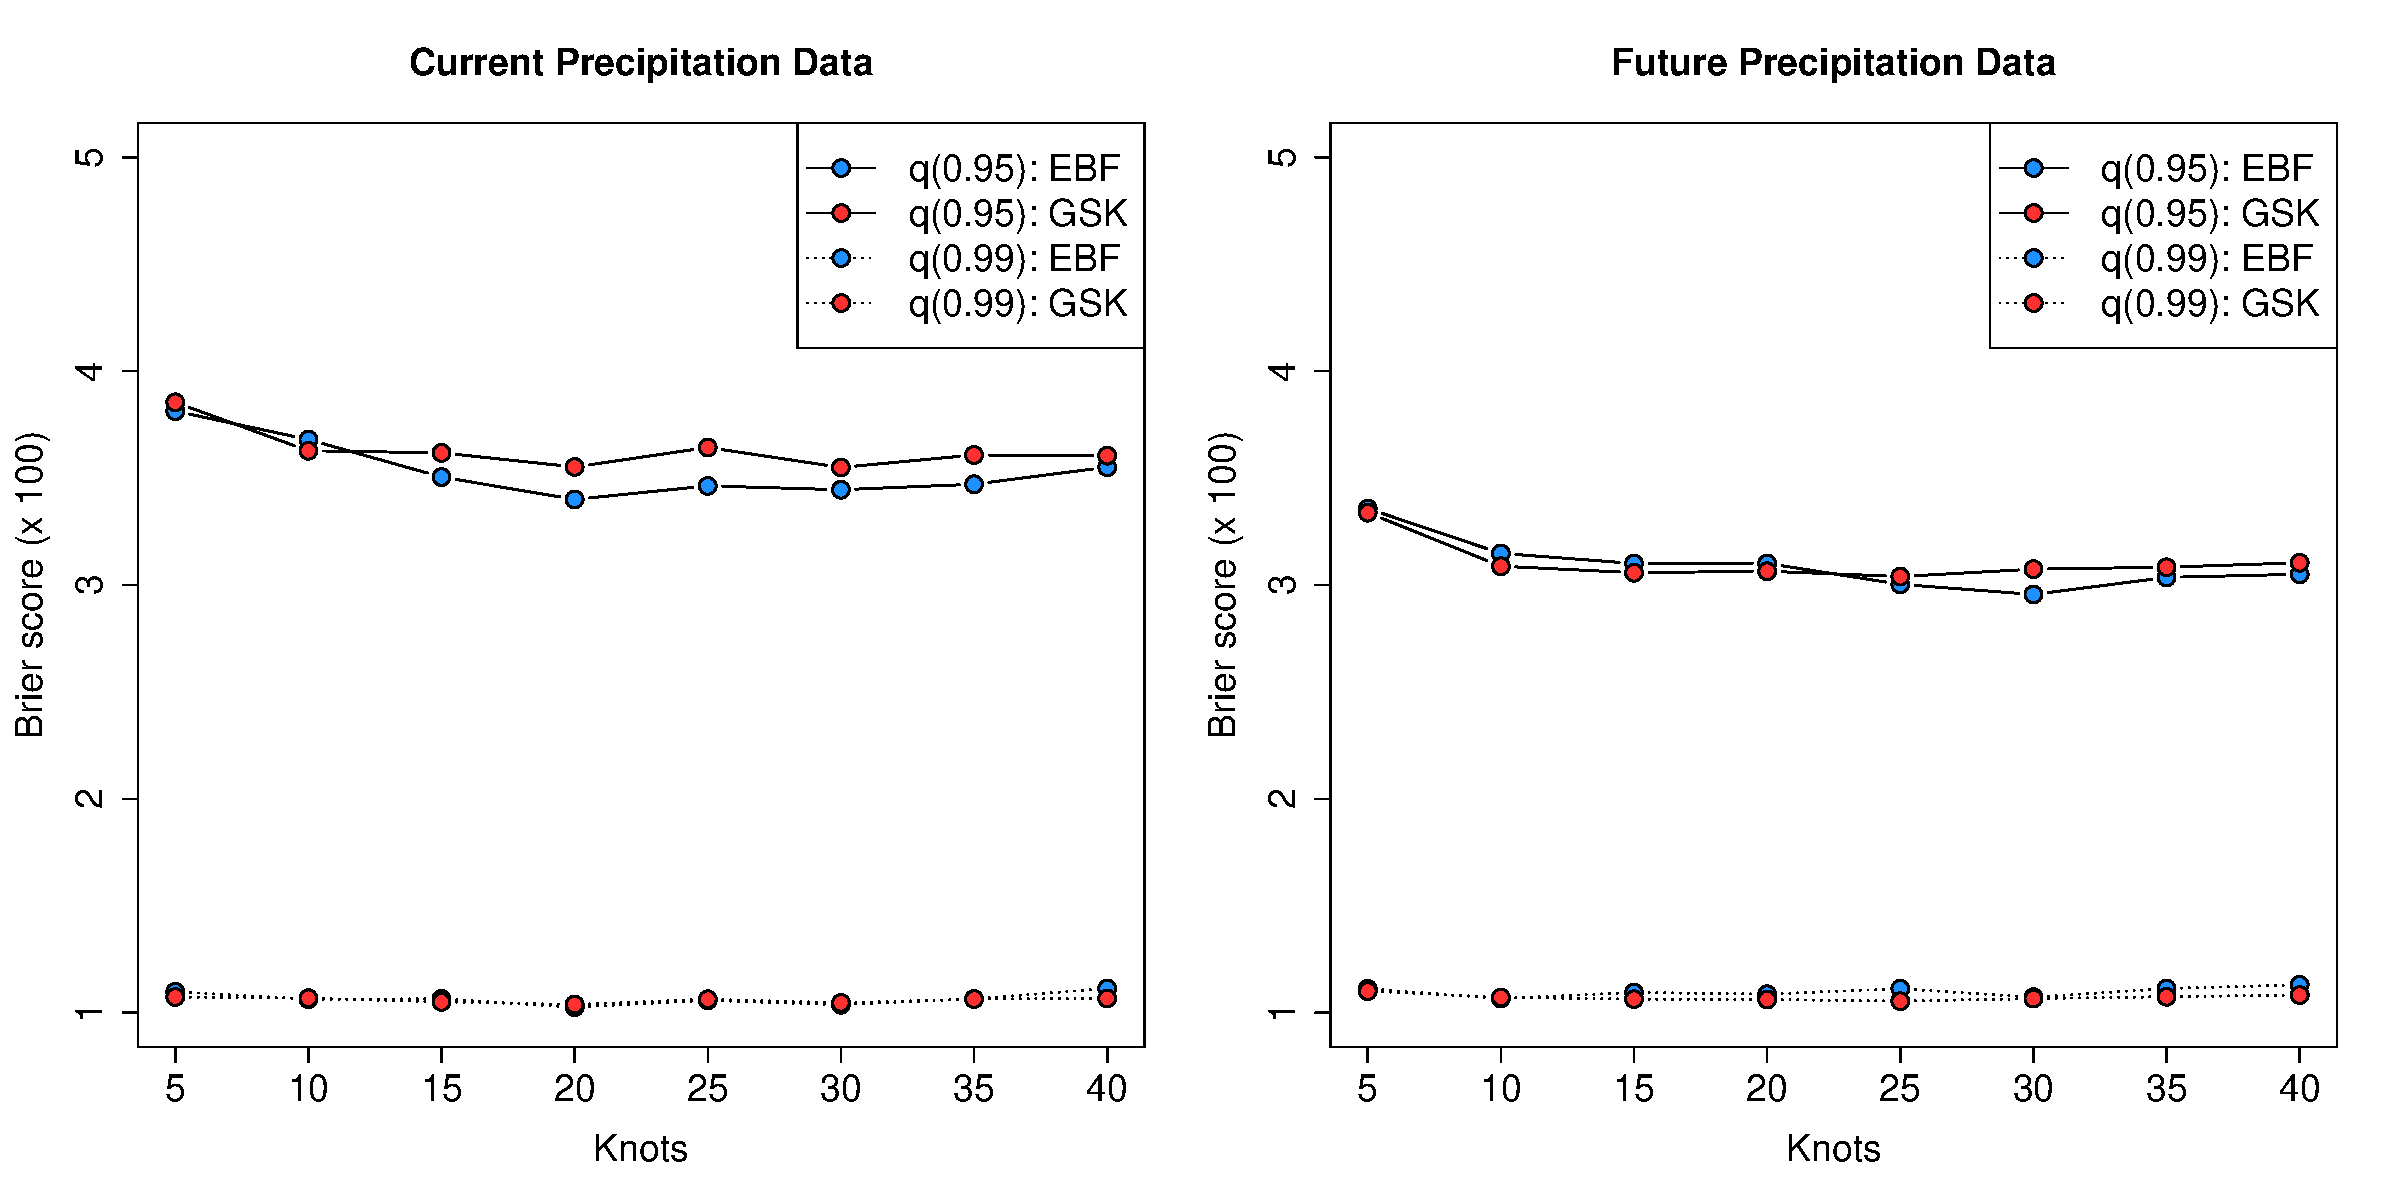
\includegraphics[width=\linewidth]{plots/precip-bs.pdf}
%   \caption{Brier scores for current and future precipitation analysis.}
%   \label{ebfig:precip-bs}
% \end{figure}

% \begin{figure}  % markdown/precipitation/combine-tables.R
%   \centering
%   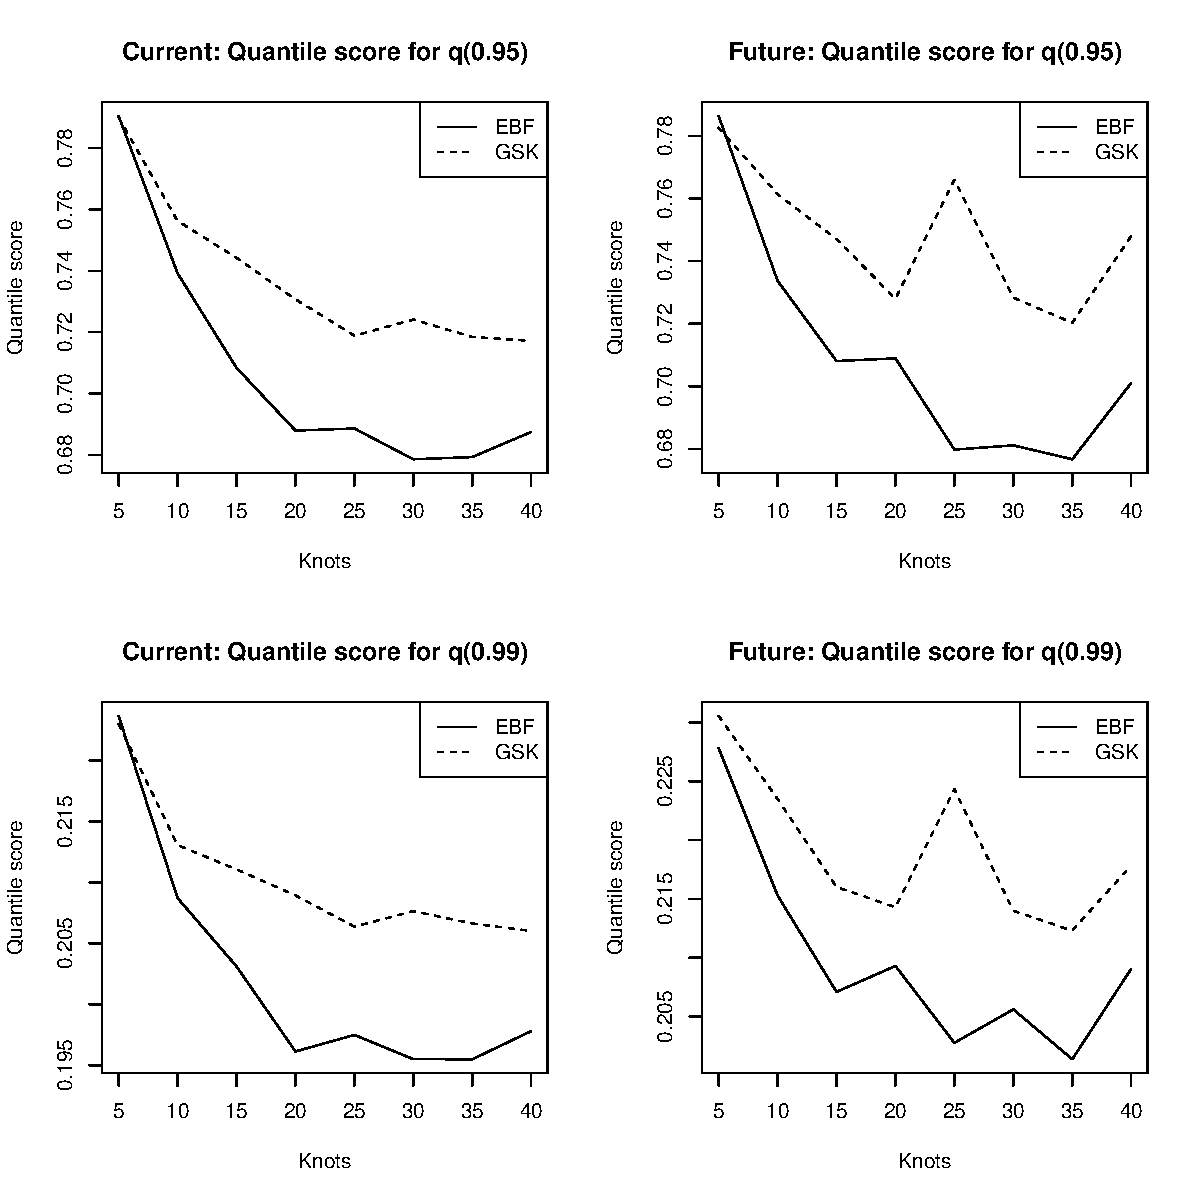
\includegraphics[width=\linewidth]{plots/precip-qs.pdf}
%   \caption{Quantile scores for current and future precipitation analysis.}
%   \label{ebfig:precip-qs}
% \end{figure}

% \begin{figure}  % markdown/precipitation/combine-tables.R
%   \centering
%   \includegraphics[width=\linewidth]{plots/precip-post-time.pdf}
%   \caption{Posterior distributions for $\beta_{\text{time}}$ for $\mu$ (left) and $\log(\sigma)$ (right).}
%   \label{ebfig:precip-qs}
% \end{figure}



\section*{Acknowledgements}
The authors would like to acknowledge Dan Cooley for his helpful suggestions on the manuscript.
The authors' work was partially supported by grants from the Department of the Interior (14-1-04-9), National Institutes of Health (R21ES022795-01A1), the US Environmental Protection Agency (R835228), the National Science Foundation (1107046).

\appendix
\section{Appendices}
\subsection{Extreme value distributions} \label{eba:GEV}

The cumulative distribution function for the GEV is $F(y) = \exp\{-t(y)\}$ where
\begin{align} \label{ebeq:gevt}
  t(y) = \begin{cases}
      \left[1 + \xi \displaystyle \frac{y - \mu}{\sigma}\right]^{-1 / \xi}, \quad &\xi \neq 0 \\
      \\
      \exp\left\{- \displaystyle \frac{y - \mu}{\sigma}\right\}, &\xi = 0.
  \end{cases}
\end{align}
The probability density function for the GEV is given by $f(y) = \displaystyle \frac{1}{\sigma} t(x)^{\xi + 1} \exp\{-t(y)\}$ where $t(y)$ is defined in \eref{ebeq:gevt}.

\subsection{Grid approximation to PS density} \label{eba:gridapprox}

The PS($\alpha$) density can be challenging to use because it does not have a closed form.
From Section 2 of \citep{Stephenson2009}, the density can be expressed as
\begin{align}
  g_1(A) = \int_0^1 g_1(A, B) \dd B,
\end{align}
where
\begin{align}
  g_1(A, B) = \frac{\alpha}{1 - \alpha} \left( \frac{1}{A} \right)^{1 / 1 - \alpha} c(\pi B) \exp \left\{ -\left(\frac{1}{A}\right)^{\alpha / (1 - \alpha)} c(\pi B) \right\},
\end{align}
with
\begin{align}
  c(\psi) = \left[\frac{\sin(\alpha \psi)}{\sin(\psi)}\right]^{1 / (1 - \alpha)} \frac{\sin[(1 - \alpha) \psi]}{\sin(\alpha \psi)}.
\end{align}
\Citet{Stephenson2009} presents an auxiliary variable technique to deal with the integral in the density function, but we opt to numerically evaluate the integral because it is only one-dimensional.
To evaluate the integral, we use 50 evenly spaced quantiles of a Beta$(0.5, 0.5)$ distribution as the midpoints $B_1, \ldots, B_{50}$, and then use the midpoint rule to evaluate $\displaystyle \int_0^1 g_1(A, B) \dd B$.

\subsection{Standardized Gaussian kernel functions} \label{eba:gskfunctions}

\citet{Reich2012} use standardized Gaussian kernel functions as their spatial basis functions in the low-rank max-stable model.
Consider a set of $\bk_1, \ldots, \bk_L$ spatial knot locations in $\calD^2$, the region of interest.
Then
\begin{align}
  \hat{B}_{il} = \frac{\exp\left\{- \displaystyle\frac{||\bs_i - \bk_l||^2}{2 \rho^2} \right\}}{\displaystyle \sum_{j = 1}^L \exp\left\{- \frac{||\bs_i - \bk_j||^2}{2 \rho^2} \right\}}
\end{align}
where $|| \cdot ||$ is the Euclidean distance between a site and a knot location.

\section{Principal components} \label{eba:pca}

As a comparison to the EBFs,  \fref{ebfig:precip-eigpanel} gives the first six principal components for the precipitation data.
These figures show that the EBFs resemble the EOFs  for the precipitation data.
%\begin{figure}[htbp] % markdown/fire-analysis/basis-functions.R
%  \centering
%  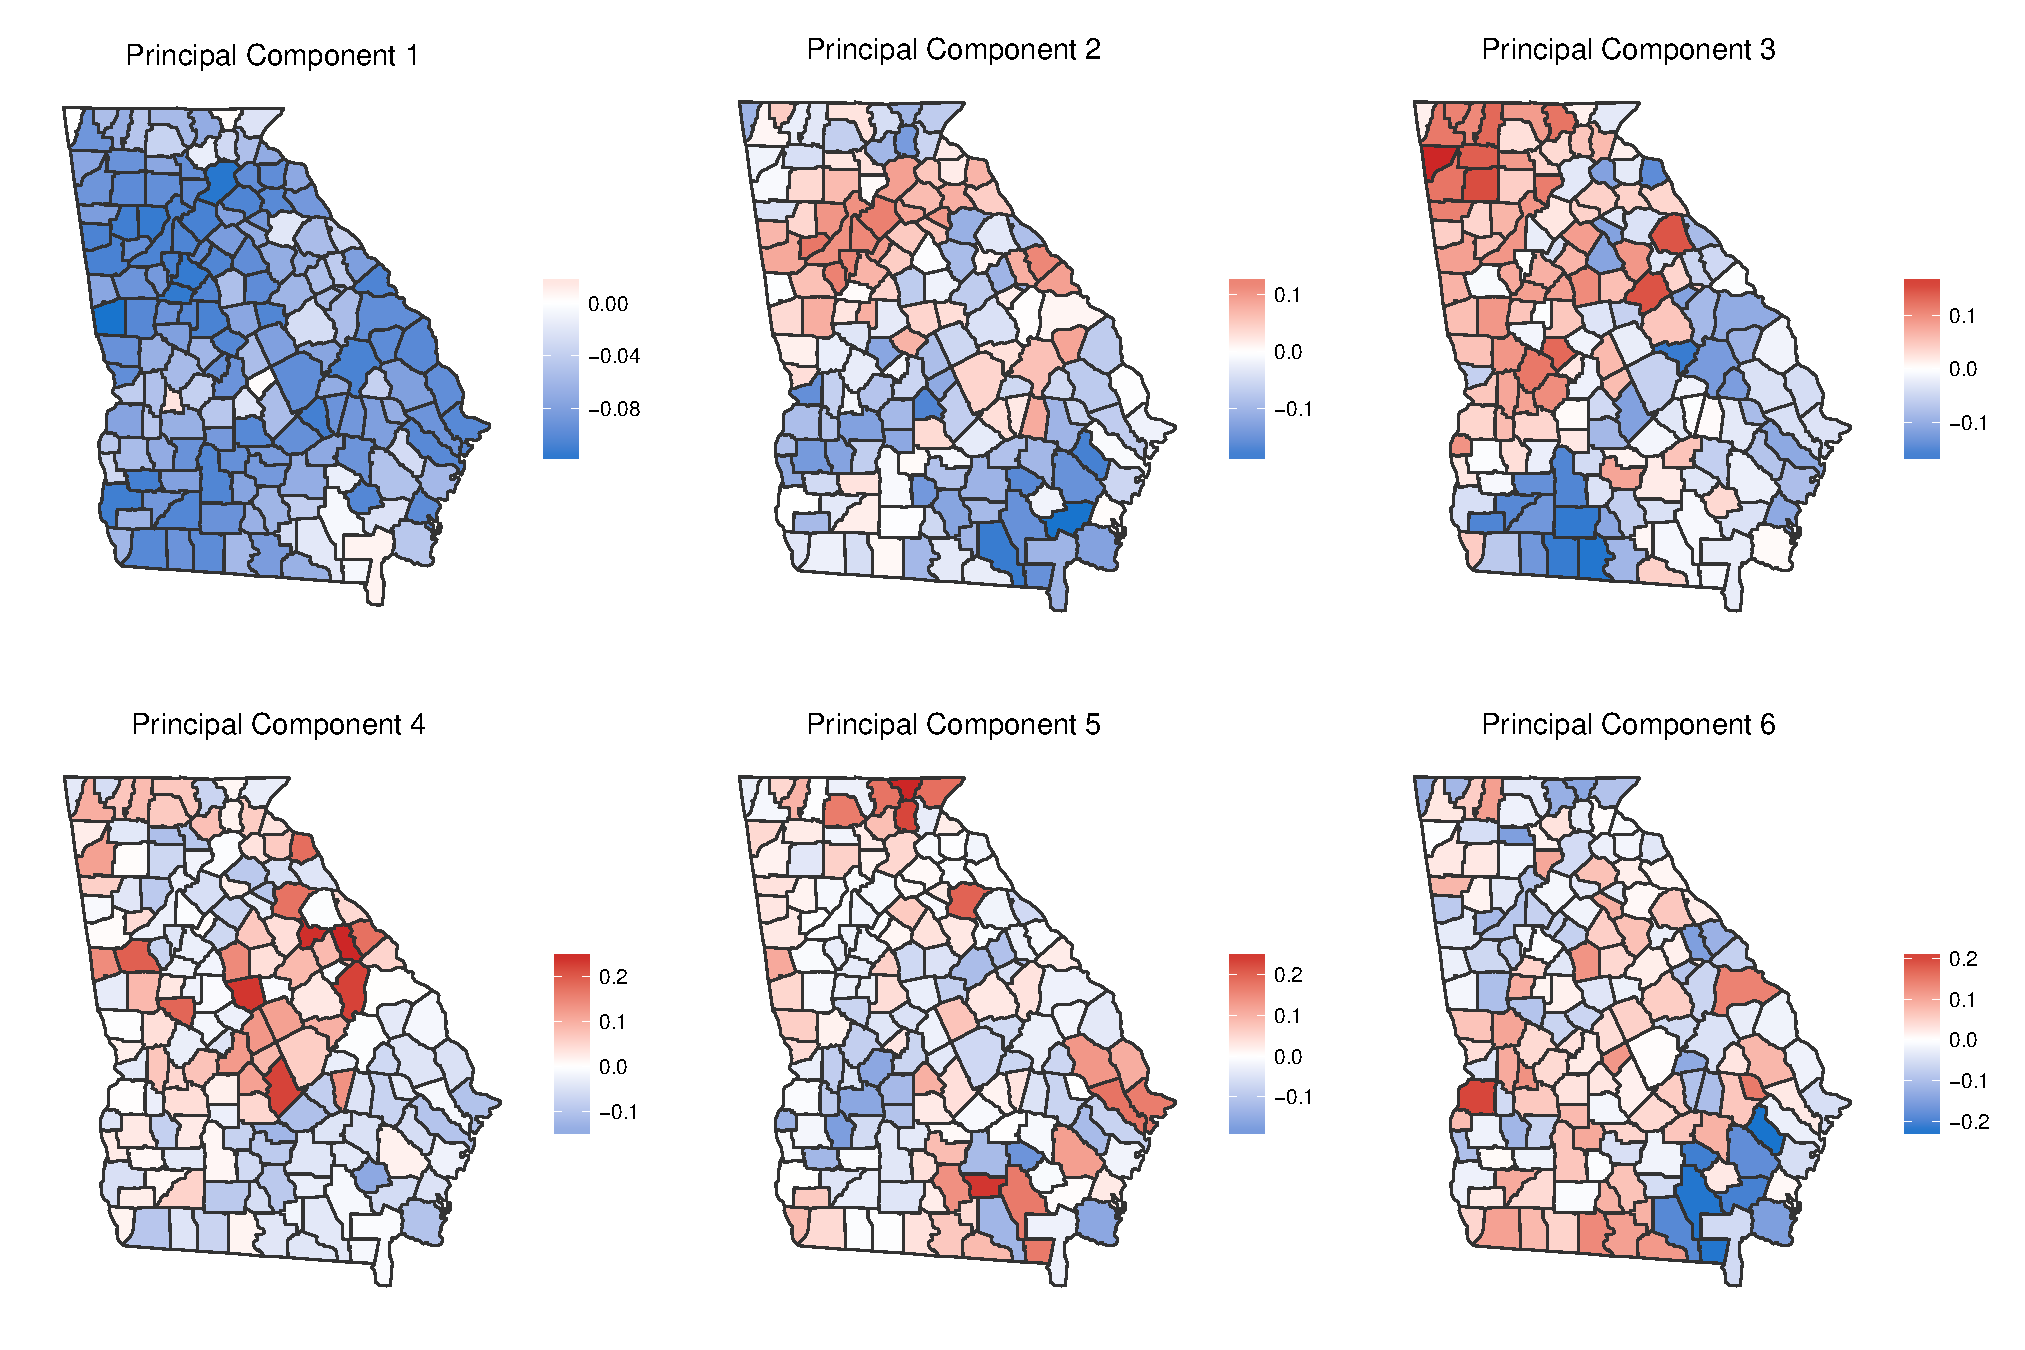
\includegraphics[width=\linewidth]{plots/fire-eig-panel.pdf}
%
%  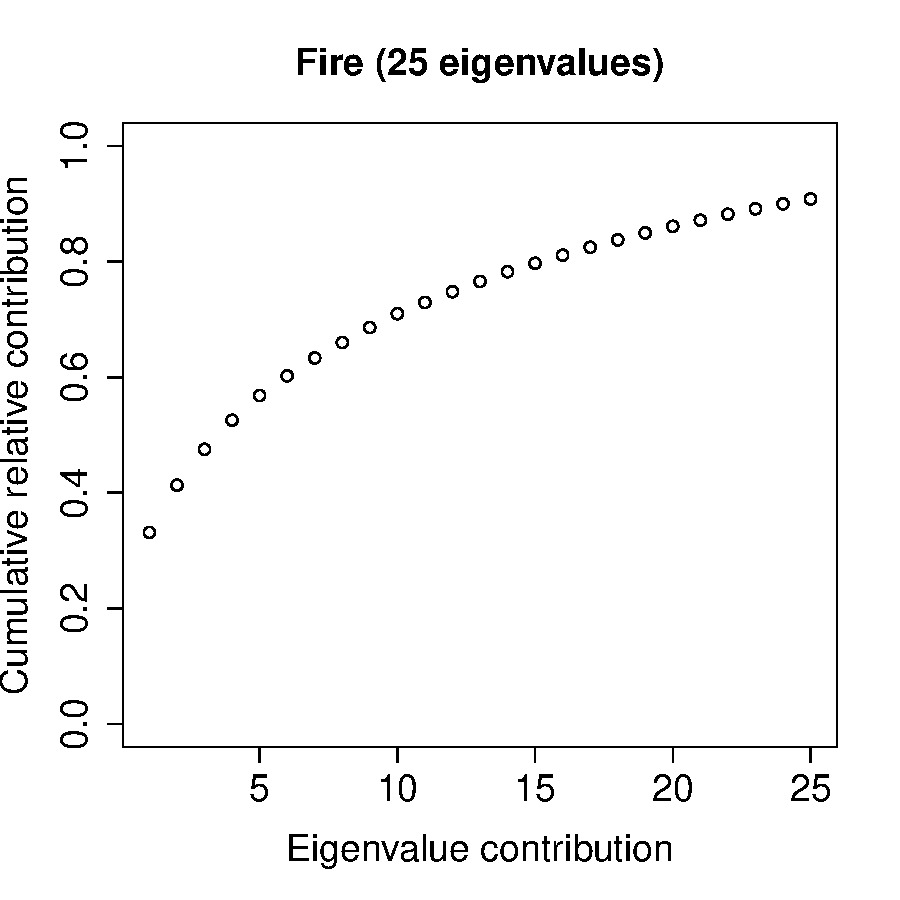
\includegraphics[width=0.35\linewidth]{plots/firelambda-25.pdf}
%  \caption{First six principal components and the cumulative sum of the first 25 eigenvalues for the Georgia fire data.}
%  \label{ebfig:fire-eigpanel}
%\end{figure}

% \begin{figure}[htbp] % markdown/fire-analysis/basis-functions.R
%   \centering
%   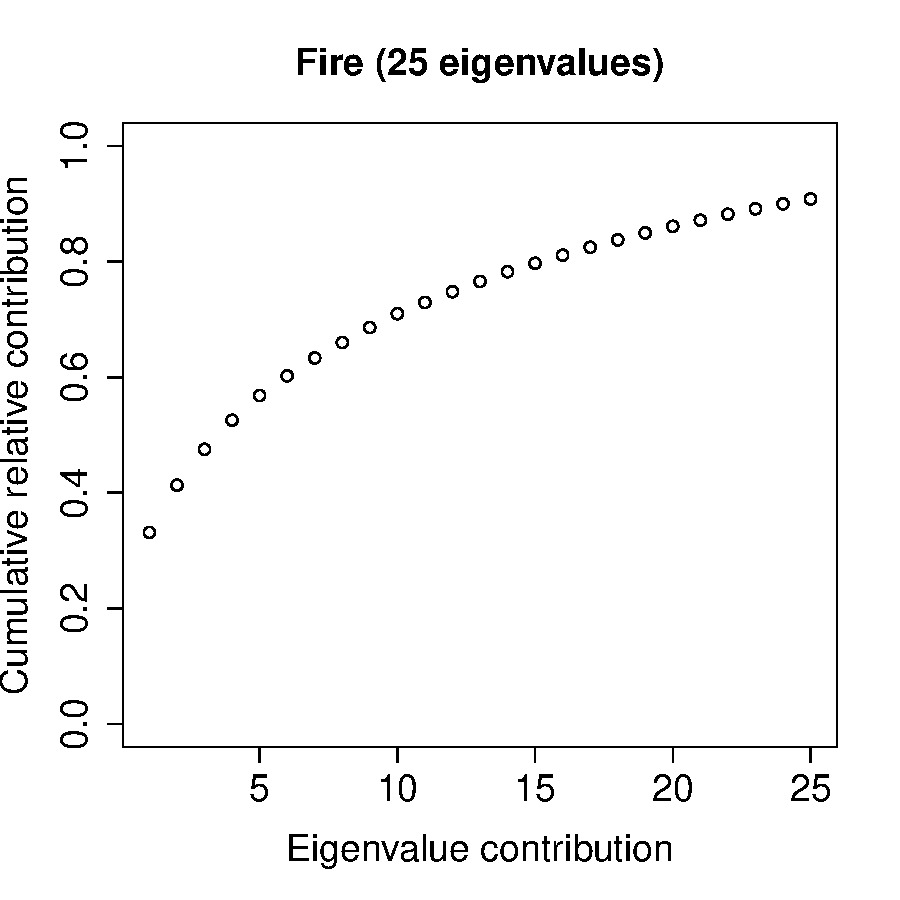
\includegraphics[width=0.5\linewidth]{plots/firelambda-25.pdf}
%   \caption{Cumulative sum of the first 25 eigenvalues.}
%   \label{ebfig:fire-eigpanel}
% \end{figure}

\begin{figure}[htbp]  % markdown/precipitation/cv-setup.R
  \centering
  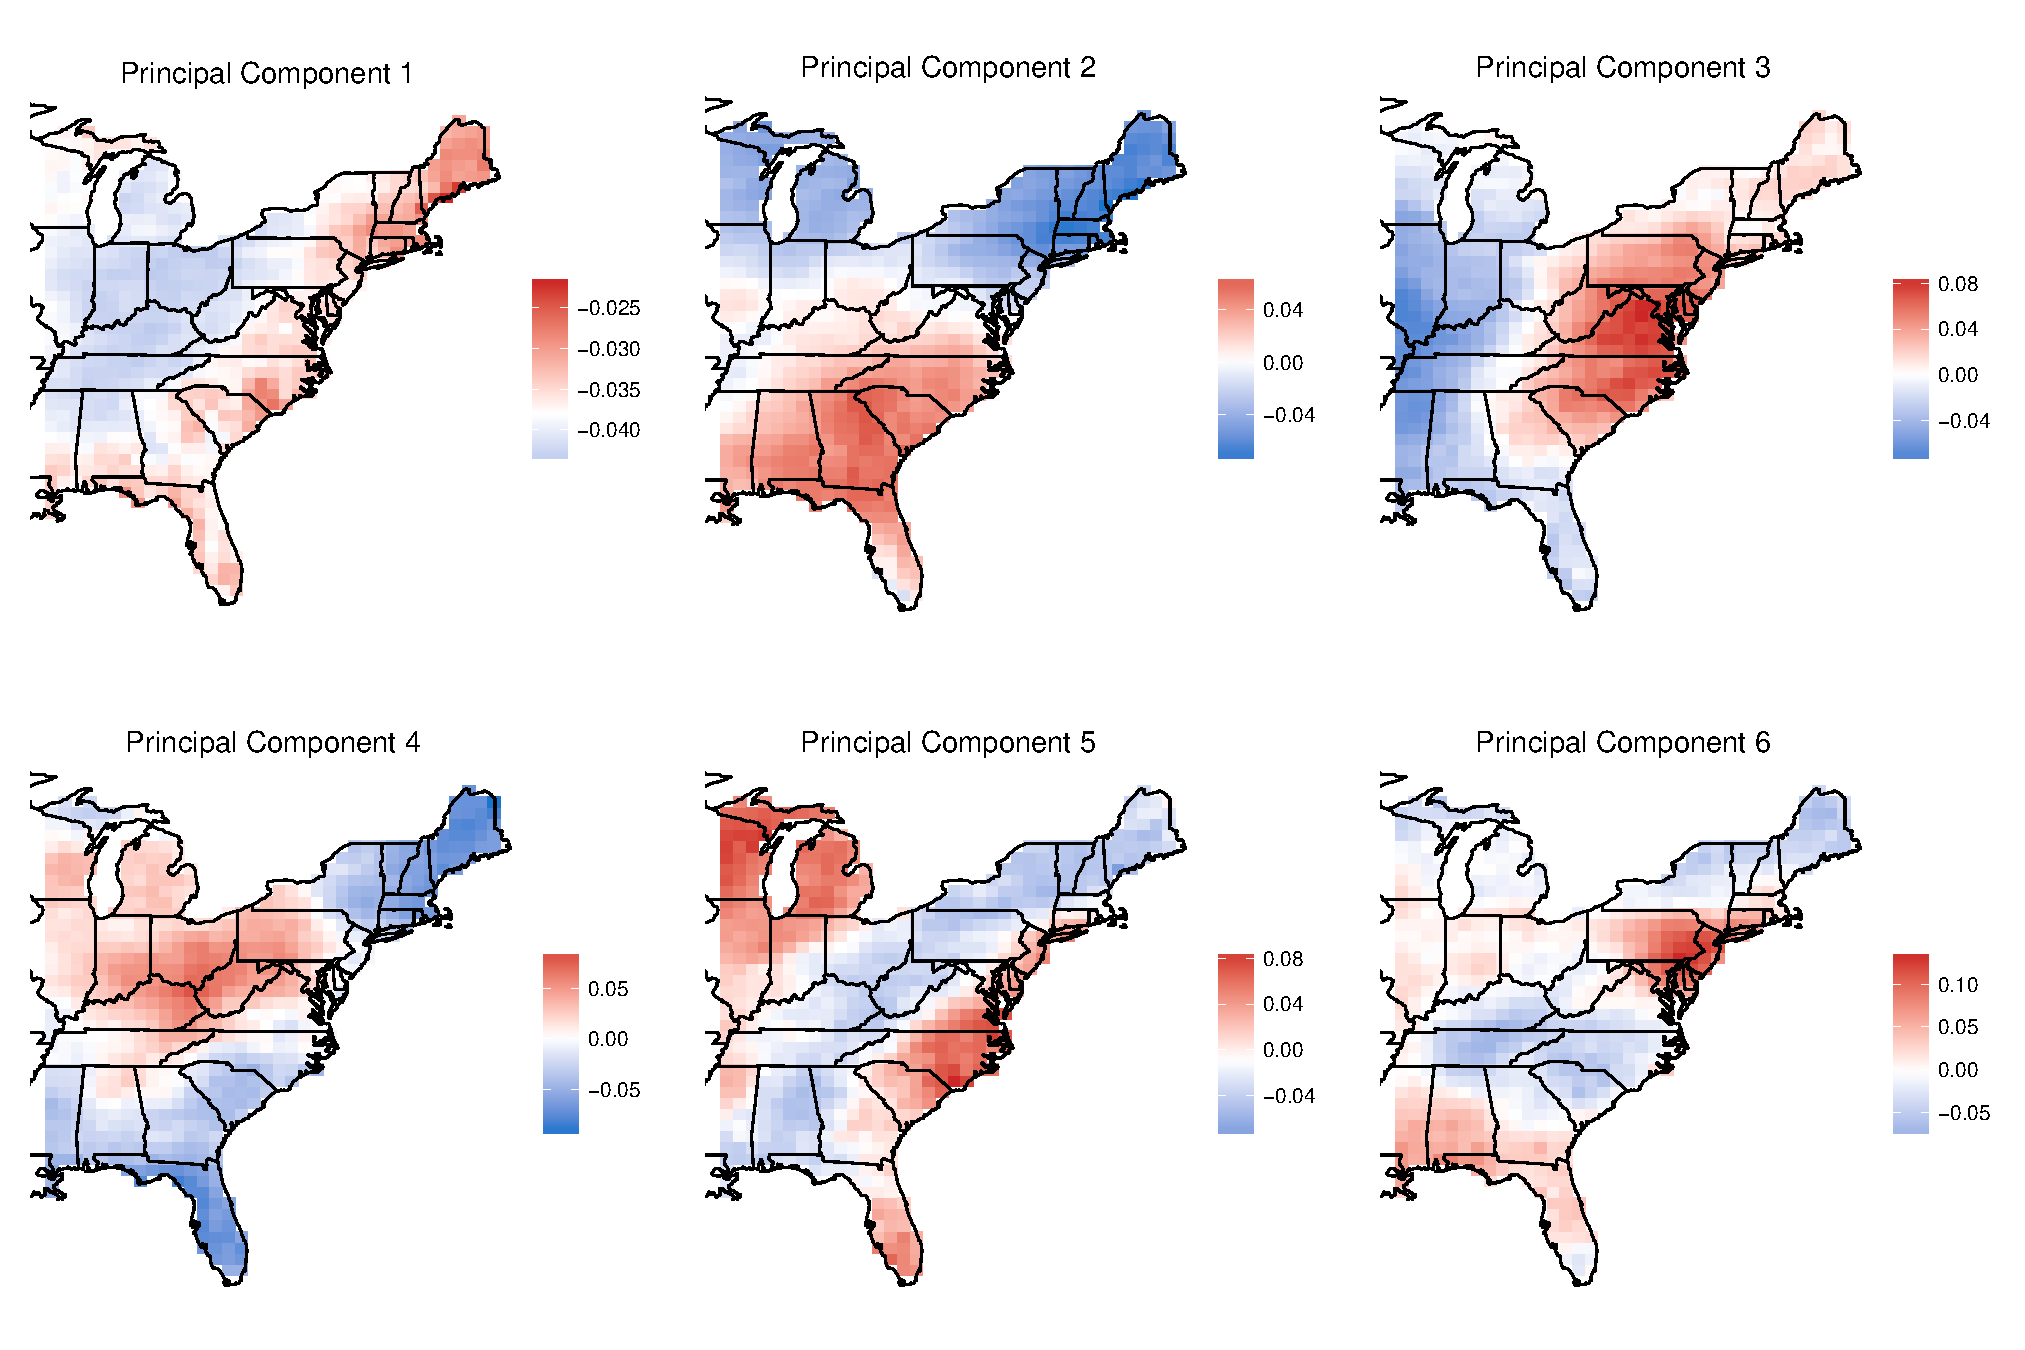
\includegraphics[width=\linewidth]{plots/precip-eig-panel.pdf}

  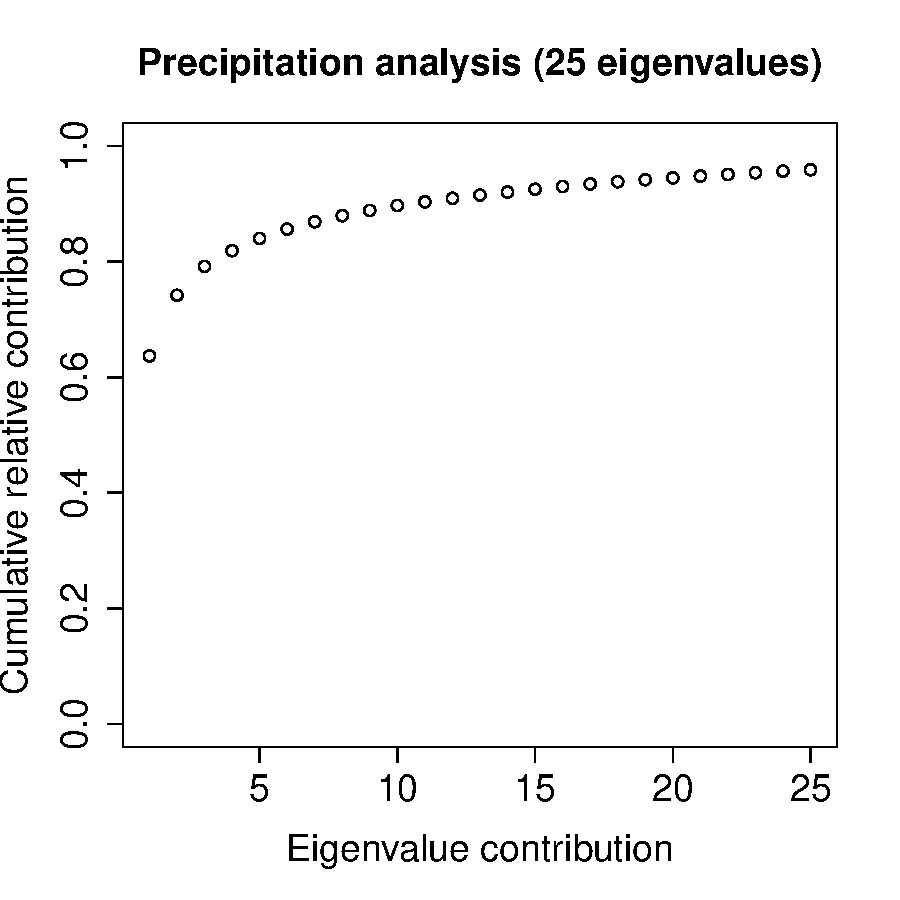
\includegraphics[width=0.35\linewidth]{plots/preciplambda-25.pdf}
  \caption{First six principal components and the cumulative sum of the first 25 eigenvalues for the precipitation data.}
  \label{ebfig:precip-eigpanel}
\end{figure}




\bibliographystyle{rss}
\bibliography{library}


\end{document}




